\documentclass[11pt, a4paper]{report}
% ===== ENCODING & LANGUAGE =====
\usepackage[utf8]{inputenc}
\usepackage[T1]{fontenc}
\usepackage[english]{babel}
\usepackage{textcomp}
\usepackage{newtxtext}
\usepackage{tikz}
\usetikzlibrary{arrows.meta, positioning, shadows.blur}

% ===== PAGE LAYOUT =====
\usepackage[paperwidth=8.5in,paperheight=11.0in,left=1.125in,right=0.875in,top=0.875in,bottom=0.875in]{geometry}
\usepackage{setspace}
\onehalfspacing
% ===== TEXT ALIGNMENT =====
\usepackage{ragged2e}
\justifying
% ===== GRAPHICS & FIGURES =====
\usepackage{graphicx}
\graphicspath{{./figures/}{./}}
\usepackage{float}
\usepackage{caption}
\usepackage{lscape}
\usepackage{pdflscape}
% ===== TABLES =====
\usepackage{longtable}
\usepackage{multirow,bigdelim,dcolumn,booktabs}
% ===== MATH =====
\usepackage{amsmath}
\usepackage{amssymb}
% ===== UNITS =====
\usepackage{siunitx}
% ===== TIKZ & DIAGRAMS =====
\usepackage{tikz}
\usetikzlibrary{shapes.geometric, arrows, decorations.pathreplacing, matrix, positioning, chains}
\usepackage{pgfgantt}
% ===== ALGORITHM =====
\usepackage[ruled,vlined]{algorithm2e}
% ===== CODE LISTINGS =====
\usepackage{listings}
\usepackage{xcolor}
\lstset{
    language=Python,
    basicstyle=\ttfamily\small,
    keywordstyle=\color{blue},
    commentstyle=\color{gray},
    stringstyle=\color{red},
    breaklines=true,
    showstringspaces=false,
    tabsize=4,
    numbers=left,
    numberstyle=\tiny\color{gray},
    frame=single
}
% ===== CITATIONS & REFERENCES =====
\usepackage{cite}
\usepackage[hidelinks]{hyperref}
% ===== FORMATTING =====
\usepackage{color}
\usepackage{titlesec}
% ===== CHAPTER FORMATTING =====
\titleformat{\chapter}[display]
  {\normalfont\bfseries\Huge}
  {\chaptertitlename\ \thechapter}{20pt}{\Huge}
\titlespacing*{\chapter}{0pt}{0pt}{40pt}
% ===== NO PARAGRAPH INDENTATION =====
\setlength{\parindent}{0pt}
\setlength{\parskip}{1em}

\begin{document}
\setlength{\parindent}{0pt}
\setlength{\parskip}{2ex plus 0.5ex minus 0.2ex}
\linespread{1.2}
\tolerance2000


\pagestyle{empty}

\begin{center}
\begin{figure}
    \centering
    
\includegraphics[width=0.8\linewidth]{biust.png}
\end{figure}
\vspace*{0.1cm}

{\large \Large \textbf{Adaptive Multi-Agent Reinforcement Learning for Traffic Signal Optimisation along the Palapye A1 Urban Corridor}}
\\


\vspace*{1.5cm}

{\large
Full Name: Tsotlhe Nayang Seiphepi\\
Student ID: 21001137\\}
Supervisor: Dr.\ Bokamoso Basutli \\
\vspace*{1.0cm}
Student Signature: \underline{\hspace{5cm}} \\
\vspace*{1.0cm}
Supervisor Signature: \underline{\hspace{5cm}} \\
\vspace*{1.0cm}

EEEN 520 - YEAR 5 SEMESTER 2\\
Department of Electrical, Computer and Telecommunications\\
Faculty of Engineering and Technology\\
Botswana International University of Science and Technology\\
Botswana, Palapye

\vspace*{0.2cm}

{\em In partial fulfillment of the requirements for the degree of Bachelor in
Computer and Telecommunications Engineering}

\vspace*{0.2cm}

{\bf 21 November 2025}

\vfill

\end{center}


\newpage
\newpage
\clearpage

% ===== FRONT MATTER =====
\newpage
\pagenumbering{roman}
\onehalfspacing
\tableofcontents
\listoftables
\listoffigures
\newpage

% ===== MAIN CONTENT =====
\pagenumbering{arabic}
\onehalfspacing

\chapter{Introduction}

Palapye has grown into both a commercial centre and a key transit town on the A1
   highway, but its traffic management has not kept up. The main junctions on the
  corridor still run fixed pre timed cycles. During peak hours, public holidays, and on high demand
  days, those static schedules cannot adjust to actual volumes, and queues build
  up as a result.

Prolonged idling raises fuel consumption and air pollution, harming the local environment and economy. Congestion at busy intersections raises accident risk. Long, unpredictable waiting times reduce quality of life for residents and undermine Palapye's development as a growing urban centre.

These challenges create a strong case for adopting a better solution. An intelligent and  adaptive traffic control system, capable of adjusting signal timing in real time. This project investigates simulation based reinforcement learning approaches as a technical foundation for future adaptive traffic control deployment in Palapye.  Evaluating their potential to reduce delays, improve throughput, and establish benchmarks on which real world implementation can be based.

\section{Background of the study}

Palapye has grown from a village into a mid sized town on the A1 highway between
   Gaborone and Francistown, the two main cities in Botswana. Its position on the
  A1 also places it on the main transit corridor between South Africa and Zimbabwe
   [2]. Major traffic generators such as the Morupule Coal Mine and the Botswana
  International University of Science and Technology add recurrent,
  time peaked demand from shift changes, deliveries, and campus activity.

 Road capacity and traffic control have not kept pace with the town's growth.
  Many signalised intersections still run on static, pre timed cycles that do not
  respond to fluctuating flows. During peak travel times, public holidays,
  university openings, and special events, queues build on the A1 and town access
  roads, increasing delays, fuel use, and local emissions. Congestion near
  junctions also raises crash risk; drivers already running late on the A1 tend to
   take risks to make up time. This study examines Palapye's traffic conditions
  and tests data driven control strategies against a fixed time baseline

\begin{figure}[H]
  \centering
  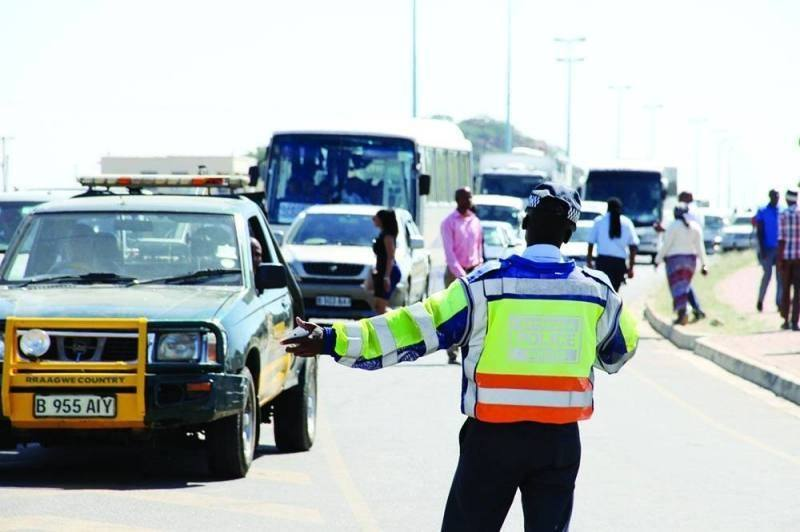
\includegraphics[width=\textwidth]{A1 TRAFFIC.jpg} 
  \caption{Traffic on the A1 road near Palapye \cite{mmegi_heavy_traffic_a1} .}
  \label{fig:traffic_a1}
\end{figure}
        
\newpage

\section{Problem Statement}

Palapye's signal controllers operate on fixed cycles with no visibility into
  actual queue lengths and no ability to coordinate phase decisions across
  adjacent junctions. During peak hours, public holidays, or incidents, queues
  spill back across junctions and green time is wasted on empty approaches.
  Real-time sensing, corridor level coordination, and adaptive phase selection are
   all absent from the current infrastructure. This project addresses those gaps.

\newpage

\section{Research Objectives}

\begin{itemize}
    \item Develop and test a YOLOv8-based vehicle detection module that identifies
  vehicles, estimates queue lengths, and extracts traffic metrics from camera
  footage, for potential integration into a future closed loop adaptive traffic
  control system.
    \item Model and simulate the three-intersection Palapye A1 corridor in SUMO with
  multi-lane geometry, a dynamic vehicle injection system, and six demand
  scenarios: off-peak, normal, morning and evening rush hour, holiday transit, and
   incident.
    \item Design and implement a Multi-Agent Deep Reinforcement Learning controller using MAPPO with a Centralised Training, Decentralised Execution architecture, where three cooperative agents share policy parameters and are jointly trained against a global cooperative reward to minimise network wide vehicle waiting time across the corridor.
    \item Quantitatively evaluate the MAPPO controller against a single-agent PPO baseline and a conventional fixed time controller across key traffic performance metrics (average waiting time, queue length, throughput, and intersection pressure) under multiple demand scenarios to validate the benefit of multi-agent coordination over single-agent and non adaptive approaches.
\end{itemize}

\section{Contributions}

This project makes the following contributions:

\textbf{Multi-agent traffic signal controller for a real Botswana road network.}  A MAPPO controller with Centralised Training, Decentralised Execution is
  designed, implemented, and evaluated on a three-intersection corridor matching
  the actual geometry of the A1 road through Palapye. This is one of the first
  applications of cooperative multi-agent deep reinforcement learning to a
  signalised arterial network infrastructure in Botswana.

\textbf{SUMO simulation environment for the Palapye A1 corridor.}A micro-simulation network is built from actual road geometry with multi-lane
  layout, turn movements, and six demand scenarios (off-peak, normal, morning
  rush, evening rush, holiday transit, incident). The environment records
  timestep-level data including queue lengths, waiting times, vehicle counts,
  signal phases, and throughput, which the Botswana Department of Roads can use
  for benchmarking and calibration once real traffic counts are available.

\textbf{Quantitative baseline for adaptive versus fixed time control in Palapye.} The evaluation provides the first quantitative comparison of fixed time, single-agent RL, and multi-agent RL control strategies on this specific corridor, establishing performance benchmarks that future work can build on.

\textbf{YOLOv8 vehicle detection pipeline.} A camera based vehicle detection and queue estimation module is implemented and validated on sample Palapye traffic footage, providing a pathway toward real world sensor integration in future deployment phases.


\section{Project Scope and Progression}
A real world deployment would require training directly on live traffic at the
  three junctions. No historical traffic data exists for Palapye intersections, so
   building a dataset from scratch would take months of live collection, camera
  calibration, and iterative signal adjustments, plus safety management,
  regulatory approval from the Botswana Department of Roads, and liability for any
   signal failures. Hardware testing also confounds signal behaviour with
  variables the controller cannot influence: sensor noise, lighting conditions,
  hardware latency, and driver routing decisions.

  A simulation based approach avoids these constraints by generating training data
   synthetically. The project runs in two phases. Phase 1 trained a single-agent
  PPO controller on one isolated intersection. Phase 2 extended this to
  the full Palapye A1 corridor, replacing the single-agent controller with a MAPPO
   system controlling all three signalised junctions under a Centralised Training,
   Decentralised Execution architecture.


\chapter{Literature Review}

\begin{figure}[H]
\centering
\makebox[\textwidth][c]{%
\resizebox{0.62\textwidth}{!}{%
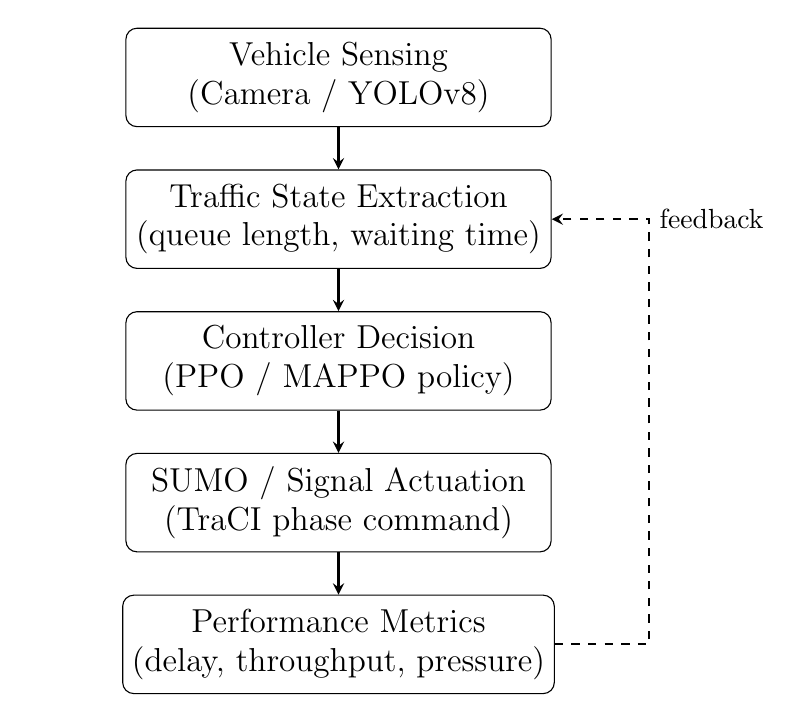
\begin{tikzpicture}[
    node distance=1.8cm,
    block/.style={rectangle, draw, rounded corners, minimum width=5.4cm, minimum height=1.25cm, align=center, fill=white, font=\large},
    >=stealth
]
\node[block] (sense)   {Vehicle Sensing\\(Camera / YOLOv8)};
\node[block, below of=sense]  (state)   {Traffic State Extraction\\(queue length, waiting time)};
\node[block, below of=state]  (ctrl)    {Controller Decision\\(PPO / MAPPO policy)};
\node[block, below of=ctrl]   (sumo)    {SUMO / Signal Actuation\\(TraCI phase command)};
\node[block, below of=sumo]   (perf)    {Performance Metrics\\(delay, throughput, pressure)};
\draw[->, thick] (sense) -- (state);
\draw[->, thick] (state) -- (ctrl);
\draw[->, thick] (ctrl)  -- (sumo);
\draw[->, thick] (sumo)  -- (perf);
\path (perf.west) -- ++(-1.2,0);
\draw[->, thick, dashed] (perf.east) -- ++(1.2,0) |- (state.east) node[midway, right]{\normalsize feedback};
\end{tikzpicture}%
}%
}
\caption{System pipeline from vehicle sensing to policy update.}
\label{fig:block_diagram_system}
\end{figure}

\section{Traffic Sensing and Vehicle Detection Technologies}

\textbf{Vehicle Detection using Camera Vision}

\cite{dos2024vehicular} detect vehicles using classical computer vision in OpenCV, with no deep learning involved. Frames from a static camera are passed through MOG2 background subtraction, which separates moving vehicles from the static background. The result is thresholded into a binary mask that marks motion against non-motion, and contour detection then traces the outlines of the moving regions. Small contours below a set area (roughly 500 to 1000 pixels) are dropped as noise, leaving only blobs large enough to be vehicles.

Each remaining contour is reduced to its centroid, and the system tracks that point against a reference line drawn across the frame. A vehicle is counted once when its centroid crosses the line within a tolerance band, which prevents the same vehicle being counted twice as it moves through the scene. This count gives a running estimate of traffic flow. \cite{dos2024vehicular} report strong accuracy on smaller vehicles (around 90 percent for cars and 100 percent for motorcycles) but weaker results on buses and trucks, where occlusion and size variation throw off the detection.

\begin{figure}[H]
\begin{center}
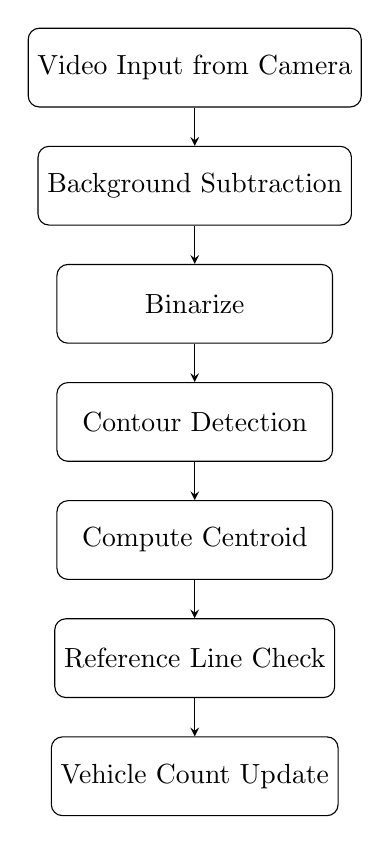
\begin{tikzpicture}[
    node distance=1.5cm,
    every node/.style={rectangle, draw, rounded corners, minimum width=3.5cm, minimum height=1cm, align=center},
    >=stealth
]

% Nodes
\node (input) {Video Input from Camera};
\node (background) [below of=input] {Background Subtraction};
\node (binarize) [below of=background] {Binarize};
\node (contour) [below of=binarize] {Contour Detection};
\node (centroid) [below of=contour] {Compute Centroid};
\node (linecheck) [below of=centroid] {Reference Line Check};
\node (count) [below of=linecheck] {Vehicle Count Update};

% Arrows
\draw [->] (input) -- (background);
\draw [->] (background) -- (binarize);
\draw [->] (binarize) -- (contour);
\draw [->] (contour) -- (centroid);
\draw [->] (centroid) -- (linecheck);
\draw [->] (linecheck) -- (count);

\end{tikzpicture}
\end{center}
\caption{Block diagram of the vehicle detection and counting system.}
\label{fig:vehicle_detection_camera}
\end{figure}

\textbf{Vehicle Detection Using Deep Learning and YOLO}
Deep learning shifted vehicle detection away from hand-crafted feature pipelines toward convolutional neural networks (CNNs) trained end-to-end on large annotated datasets. Classical methods like background subtraction only pull moving blobs out of a video. A CNN instead learns to tell vehicle classes apart (car, truck, motorcycle, bus) straight from raw pixels, and it holds up across lighting, occlusion, and camera angles that a classical pipeline would need retuning for \cite{futuretransp5040137}.

The most common family of real time detectors is YOLO (You Only Look Once). Two-stage detectors like Faster R-CNN first propose regions of interest and then classify each one. YOLO instead treats detection as a single regression problem: it takes the whole image at once and predicts bounding boxes and class probabilities across a spatial grid in one forward pass. That single-stage design is what makes it fast enough for live camera feeds at an intersection. YOLOv8, the version used here, uses an anchor-free detection head that predicts object centres directly instead of offsets from preset anchor boxes. This improves recall on small objects and cuts down the hyperparameters you have to tune for a given site \cite{futuretransp5040137}.

In traffic monitoring, YOLO is usually paired with a tracker such as SORT (Simple Online and Realtime Tracking) or DeepSORT, which keeps a consistent identity for each detection across frames. With tracking in place the system can do more than count vehicles. It can measure queue length (how many detected vehicles are stationary on each approach), estimate per-vehicle waiting time, and read off direction of travel. Those are exactly the inputs a data driven signal controller needs.

The main catch with deep learning detectors is that they need labelled training data and enough compute to run in real time at a usable frame rate. On mid-range GPU hardware YOLOv8 clears 100 frames per second, well beyond what intersection monitoring requires, but that does set a floor on the processing unit you install in the field. For this project the CameraVision module runs YOLOv8 and was validated on sample traffic footage (Section~\ref{fig:yolo_detection}). Wiring it into the live SUMO training loop is left as future work.

Table~\ref{tab:opencv_yolo} compares the classical OpenCV background subtraction approach with YOLOv8 across the criteria most relevant to an outdoor intersection deployment, justifying the selection of YOLOv8 for this project.

\begin{table}[H]
\centering
\caption{Comparison of OpenCV MOG2 and YOLOv8 for traffic monitoring}
\label{tab:opencv_yolo}
\normalsize
\setlength{\tabcolsep}{7pt}
\begin{tabular}{p{3.9cm}p{4.5cm}p{4.5cm}}
\toprule
\textbf{Criterion} & \textbf{OpenCV MOG2} & \textbf{YOLOv8} \\
\midrule
Lighting robustness & Poor: shadows and headlights cause false detections & Good: trained on diverse lighting conditions \\
Occlusion handling & Poor: merged blobs for overlapping vehicles & Good: bounding-box instance separation \\
Detection accuracy & Moderate ($\sim$90\% cars, lower for trucks) & High ($>$90\% across vehicle classes) \\
Queue length estimation & Indirect via blob count & Direct via stationary bounding-box count \\
Computational cost & Low (CPU only) & Moderate (GPU recommended) \\
Ease of deployment & High: no training required & Moderate: requires pretrained weights \\
Selected for project & No & \textbf{Yes} \\
\bottomrule
\end{tabular}
\end{table}

\textbf{Vehicle Detection Using LiDAR}
In ``LiDAR-Enhanced Connected Infrastructures: Sensing and Broadcasting High-Resolution Traffic Information Serving Smart Cities'' \cite{lv2019lidar}, the authors detect, classify, and track vehicles and pedestrians in real time using LiDAR alone. Their sensor, a Velodyne VLP-16, spins multiple laser beams through a full 360 degrees and returns up to 600,000 distance points per second out to roughly 100 meters. Every reflected pulse comes back as a 3D coordinate (x, y, z), so the sensor effectively rebuilds the shape of the road in front of it. Mounted at the roadside around 7 to 9 feet up, it captures the full 3D profile of every moving road user in view, and it does so regardless of light or weather \cite{lv2019lidar}.

Detection works off the point cloud the spinning beams produce. Because each pulse measures distance to whatever surface it hits, a car shows up as a dense cluster of returns sitting above the ground.

First comes background filtering: stationary surfaces like the road and surrounding buildings are stripped out across several frames, leaving only the points that move. DBSCAN clustering then groups the remaining points by spatial density, and each cluster is taken to be one object, a car, a pedestrian, or a cyclist \cite{lv2019lidar}.

For each cluster the system pulls out geometric features (point count, width, height, and distance from the sensor) and feeds them to a Random Forest classifier trained to separate vehicles from pedestrians. The cue is shape: vehicles give broader, lower, denser clusters, while a pedestrian reads as a narrow upright one.

Once a cluster is labelled a vehicle, its footprint is fitted with a minimum-area rectangle and its motion is followed frame to frame using a Kalman filter with Global Nearest Neighbor association. The result is a clean, continuous trajectory for every vehicle inside the LiDAR's 100-meter range \cite{lv2019lidar}.

\begin{figure}[H]
\begin{center}
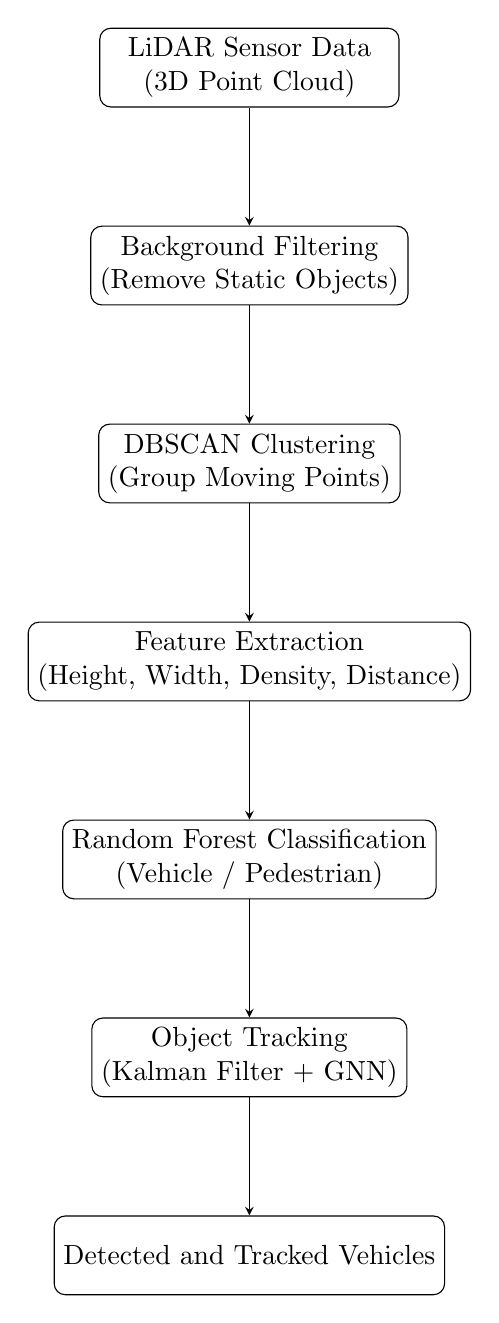
\begin{tikzpicture}[
    node distance=1.5cm,
    every node/.style={rectangle, draw, rounded corners, align=center, minimum width=3.8cm, minimum height=1cm},
    >=stealth
]

% Nodes
\node (input) {LiDAR Sensor Data\\(3D Point Cloud)};
\node (filter) [below=of input] {Background Filtering\\(Remove Static Objects)};
\node (cluster) [below=of filter] {DBSCAN Clustering\\(Group Moving Points)};
\node (features) [below=of cluster] {Feature Extraction\\(Height, Width, Density, Distance)};
\node (classify) [below=of features] {Random Forest Classification\\(Vehicle / Pedestrian)};
\node (track) [below=of classify] {Object Tracking\\(Kalman Filter + GNN)};
\node (output) [below=of track] {Detected and Tracked Vehicles};

% Arrows
\draw[->] (input) -- (filter);
\draw[->] (filter) -- (cluster);
\draw[->] (cluster) -- (features);
\draw[->] (features) -- (classify);
\draw[->] (classify) -- (track);
\draw[->] (track) -- (output);

\end{tikzpicture}
\end{center}
\caption{Block diagram of the LiDAR based vehicle detection system.}
\label{fig:lidar_detection}
\end{figure}

\textbf{Vehicle Detection Using Radio Waves and Microwaves}
Radar and microwave sensors find vehicles by sending out electromagnetic waves and reading what bounces back. Since none of this depends on visible light, they work just as well at night as during the day, and rain, fog, or dust does not bother them the way it does a camera or a LiDAR unit. That makes them a strong fit for outdoor sites with rough weather or weak lighting.

Doppler radar reads speed off the frequency shift between the wave it sends and the wave it gets back. A vehicle moving toward the sensor squeezes the reflected wave to a higher frequency; one moving away stretches it lower. How big the shift is tells you the vehicle's radial velocity, so you get an instant speed reading with no image processing involved \cite{lv2019lidar}.

Microwave presence detectors work the other way. Instead of tracking a Doppler shift, they watch the standing wave pattern at the antenna. With no vehicle around, the reflected wave lines up constructively with the transmitted one. A vehicle sitting in the detection zone breaks that pattern, and the change in signal is what registers as a detection. This is the principle behind most inductive-loop replacements and stop-bar detectors at signalised intersections \cite{michailidis2025traffic}.

Against cameras, radar and microwave have the advantage of producing no imagery at all, so road user privacy is preserved. Against LiDAR, they are cheaper and need far less post-processing. Where they fall short is spatial resolution: radar can tell you speed and presence but cannot pick apart vehicle types the way a camera or LiDAR can. For signal control that gap rarely matters, since the controller mostly wants queue length and arrival rate rather than a detailed vehicle classification.

Camera vision was selected over LiDAR and radar for this project due to its lower hardware cost, simpler roadside installation, and the availability of sample Palapye traffic footage for independent validation.\\

\section{Traffic Flow Fundamentals}

Before reviewing control strategies, it is useful to establish the fundamental measures and relationships that define how traffic behaves at a signalised intersection. These metrics are what any control policy, whether fixed time or adaptive, is ultimately trying to optimise.

\subsection{Traffic Flow Parameters}

Three quantities describe the state of traffic on a road segment at any given time. \textit{Flow} $q$ (vehicles per hour) is the rate at which vehicles pass a fixed point. \textit{Density} $k$ (vehicles per kilometre) is the number of vehicles occupying a unit length of road. \textit{Speed} $v$ (kilometres per hour) is the mean speed of the vehicle stream. These three are related by the fundamental equation of traffic flow \cite{tang2019global}:

\begin{equation}
q = k \cdot v
\label{eq:fundamental}
\end{equation}

At low density, vehicles travel freely and speed is high. As density increases, interactions between vehicles force speeds down. At jam density $k_j$, traffic is stationary and flow falls to zero. The capacity of a road section is the maximum flow it can sustain, occurring at some intermediate density.

\subsection{Saturation Flow and Degree of Saturation}

At a signalised intersection, vehicles can only depart during the green phase. The \textit{saturation flow rate} $s$ is the maximum rate at which queued vehicles discharge when the signal is green, measured in vehicles per hour of green time. It depends on lane width, turning movements, and the proportion of heavy vehicles.

The \textit{degree of saturation} $x$ for a lane group is the ratio of the demand flow to the maximum flow the signal can serve:

\begin{equation}
x = \frac{q}{s \cdot g/C}
\label{eq:saturation}
\end{equation}

where $g$ is the effective green time allocated to that lane group and $C$ is the signal cycle length. When $x < 1$ the lane group is under saturated and queues clear each cycle. When $x \geq 1$ residual queues grow from cycle to cycle, eventually leading to the spillback and gridlock that adaptive signal control aims to prevent.

\subsection{Webster's Optimal Cycle Length}

Webster's formula \cite{tang2019global} gives the cycle length $C^*$ that minimises average vehicle delay at an isolated intersection under fixed time control:

\begin{equation}
C^* = \frac{1.5L + 5}{1 - \sum_i y_i}
\label{eq:webster}
\end{equation}

where $L$ is the total lost time per cycle (the sum of start-up losses and inter-green periods across all phases), and $y_i = q_i / s_i$ is the flow ratio for the critical lane group in phase $i$. The denominator represents the spare capacity of the intersection: as the sum of flow ratios approaches 1, the optimal cycle length grows without bound and the intersection approaches saturation.

Webster's formula is derived under the assumption of steady, uniform demand. It is the theoretical basis for fixed time signal plans but breaks down when demand is variable or when vehicles arrive in platoons. Those are exactly the conditions where adaptive control provides its advantage.

\subsection{Level of Service}

The Highway Capacity Manual defines Level of Service (LOS) as a letter grade from A to F that describes the quality of traffic flow at an intersection, based on average control delay per vehicle \cite{michailidis2025traffic}:

\begin{table}[H]
\centering
\caption{Level of Service thresholds for signalised intersections}
\label{tab:los}
\begin{tabular}{cc}
\toprule
\textbf{LOS} & \textbf{Average control delay (s/vehicle)} \\
\midrule
A & $\leq 10$ \\
B & $> 10$ to $25$ \\
C & $> 25$ to $35$ \\
D & $> 35$ to $55$ \\
E & $> 55$ to $80$ \\
F & $> 80$ \\
\bottomrule
\end{tabular}
\end{table}

LOS A represents free-flow conditions with negligible delay. LOS F indicates that demand exceeds capacity and queues grow without bound. The goal of traffic signal optimisation is to maintain LOS C or better on all approaches under typical demand conditions and to limit the extent and duration of LOS E or F during peak periods. This project tracks three metrics as proxies for LOS waiting time, queue length, and throughput. In the simulation,the first two also stand in for control delay, so any controller that lowers their mean values is improving the LOS that drivers actually see at the Palapye intersections.

\section{Processing and Control Logic}

\subsection{Fixed-Time Control Method}

This technique relies on predetermined schedules for signal phases, where the green, yellow, and red times are fixed in advance. It has been shown to be effective in environments with stable and predictable traffic flows due to its simplicity and ease of implementation. However, the method does not adapt to real time fluctuations in traffic demand. As a result, its performance deteriorates under conditions of variable density, such as during accidents, special events, or sudden surges in demand \cite{michailidis2025traffic}. There are three common types of fixed time control methods \cite{tang2019global}:

\begin{enumerate}
    \item \textbf{Isolated Fixed-Time Control}: Each intersection operates on its own predetermined schedule, with no coordination between adjacent intersections.
    \item \textbf{Coordinated Fixed-Time Control}: Intersections are synchronized to create a green wave progression along major corridors, improving traffic flow over longer stretches.
    \item \textbf{Time of Day Control}: Signal schedules vary by predefined time periods (e.g., morning peak, off-peak, evening rush), but remain non responsive to live traffic conditions.
\end{enumerate}

\subsection{Actuated Control Method}

Actuated control adjusts signal timings on the fly using live sensor input from loop detectors, cameras, and infrared devices \cite{kalavsova2022impact}. A fixed time system just runs a preset schedule. Actuated control instead reacts to the vehicles actually arriving, holding a green phase longer when it still sees vehicles inside the extension window. That responsiveness keeps the intersection running more efficiently, with less idling and fewer abrupt stops.

Kalašová \cite{kalavsova2022impact} looked at how actuated control affects both traffic flow and the environment, measuring average delay, queue length, fuel consumption, and emissions. The average delay per vehicle was defined as:

\begin{equation}
d = \frac{\sum (t_{\text{actual}} - t_{\text{free}})}{N}
\label{eq:average-delay}
\end{equation}

where $t_{\text{actual}}$ is the actual travel time, $t_{\text{free}}$ is the free-flow travel time, and $N$ is the number of vehicles observed.

Queue length was measured as the accumulation of vehicles at red signals, while environmental indicators such as fuel consumption and emissions were modeled as functions of idling time and acceleration cycles.

The study showed that actuated control, which adjusts traffic signals based on real time traffic, significantly cuts down on delays and queue lengths compared to fixed time signals, especially in variable or moderate traffic conditions. It also reduces idling and stop and go driving, leading to lower CO$_2$ emissions and fuel use. However, in heavily congested, over saturated conditions, actuated control alone is not enough to fully resolve congestion or delays.

Overall, research highlights actuated signal control as a substantial improvement over fixed time methods, especially in urban environments where traffic demand fluctuates throughout the day \cite{kalavsova2022impact}.

\subsection{Adaptive Control Method}

Adaptive control is the most capable category of traffic signal management. Unlike fixed time and actuated methods, adaptive systems continuously monitor network wide traffic density and apply algorithmic models to optimise signal timings across multiple intersections in real time \cite{mannion2016experimental}. The result is a controller that responds to conditions no preset schedule could anticipate, such as sudden congestion, incidents, or atypical demand patterns that fall outside any programmed time of day profile.

Adaptive methods split into two categories \cite{ye2019survey}. Model based systems build an explicit mathematical representation of traffic flow and solve an optimisation problem over that model at each control step. Model free systems skip the model entirely and learn control policies directly from observed traffic data. The sections below cover both.

\section{Model-Based Optimization Systems}

These systems use mathematical models to represent how traffic behaves. Instead of trial and error, they predict what traffic will look like and then decide the best traffic signal timings. Common approaches include:

\subsection{Model Predictive Control}

This technique predicts future traffic states like queue lengths and delays over a finite prediction horizon and computes the best signal timings in advance. A mathematical model predicts how traffic will evolve if certain green/red timings are applied. An optimisation problem is solved to minimise a cost function subject to constraints like minimum green time or safety rules. The first part of the optimised signal plan is implemented. The process repeats at the next step with updated traffic data \cite{ye2019survey}. Mathematically, the MPC problem is expressed as:

\begin{equation}
\min_{u(0), \dots, u(N-1)} \sum_{k=0}^{N-1} J(x(k), u(k)) + J_f(x(N))
\label{eq:mpc-objective}
\end{equation}

subject to:

\begin{equation}
x(k+1) = f(x(k), u(k)) + d(k), \quad x(k) \in X, \; u(k) \in U
\label{eq:mpc-constraint}
\end{equation}

where:

\begin{itemize}
    \item $x(k)$ represents the traffic state (e.g., queue lengths or densities)
    \item $u(k)$ is the control action (signal timings)
    \item $d(k)$ is the demand disturbance
\end{itemize}

The stage cost $J(x,u)$ typically combines queue lengths, waiting times, or number of stops, while $J_f(x(N))$ serves as a terminal cost penalizing undesirable end states.

MPC can anticipate future conditions, explicitly handle multi-variable intersections and constraints, and outperforms fixed and actuated control strategies \cite{ye2019survey}. Distributed and hierarchical MPC variants also offer improved coordination across multiple intersections.

These benefits come with significant trade-offs. Centralised MPC carries a computational burden that restricts real time feasibility in large urban networks, and its performance is heavily dependent on how accurately the underlying traffic model captures reality. Most applications remain at the simulation stage, with few large scale real world deployments to date. Scalability and robustness to uncertainty remain open challenges \cite{ye2019survey}.

\subsection{Dynamic Traffic Assignment (DTA)}

Dynamic Traffic Assignment (DTA) extends static traffic assignment by considering the time-varying nature of traffic demand and network conditions. The goal is to allocate vehicles dynamically across available routes to minimise congestion and balance traffic loads. Unlike static methods, which assume fixed flows, DTA accounts for fluctuations in demand, travel times, and congestion propagation throughout the network. This makes it suitable for analyzing real world urban environments where traffic conditions evolve continuously \cite{elimadi2024review}.

Dynamic Traffic Assignment (DTA) is often formulated as a Dynamic User Equilibrium (DUE), where no driver can improve their travel time by unilaterally changing routes. The optimisation problem can be expressed as \cite{elimadi2024review}:

\begin{equation}
\min_{x} \sum_{a \in A} \int_{0}^{x_a(t)} c_a(s)\,ds
\label{eq:dta-objective}
\end{equation}

subject to:

\begin{equation}
\sum_{p \in P_{od}} h_p(t) = d_{od}(t), \quad \forall (o,d) \in OD
\label{eq:dta-constraint}
\end{equation}

where:

\begin{itemize}
    \item $x_a(t)$ is the flow on link $a$ at time $t$
    \item $c_a(s)$ is the travel cost (delay) on link $a$ as a function of flow
    \item $h_p(t)$ is the departure rate on path $p$
    \item $d_{od}(t)$ is the time-dependent travel demand between origin $o$ and destination $d$
\end{itemize}

At user equilibrium, all routes used between an origin--destination pair have equal and minimal travel times, meaning no individual driver can reduce their travel time by switching routes.

The findings of the paper \cite{elimadi2024review} indicated that the DTA can model how drivers change routes over time and how congestion builds across a city. It shows where traffic will flow, where bottlenecks form and how control strategies affect the whole system. Best use case for planning, tolling, ramp metering and signal coordination. However limitations of the model indicate that it needs detailed forecasts and accurate models of driver behavior which are very hard to obtain. It becomes computationally heavy in larger cities, making real time use difficult. The model does not handle unexpected results such as accidents and sudden traffic.

\subsection{Mixed-Integer Linear Programming (MILP)}

This approach formulates the problem of scheduling green, yellow, and red phases as a set of linear equations and inequalities, with decision variables representing signal timings. Some variables are continuous (e.g., cycle lengths, green time durations), while others are integer or binary (e.g., whether a phase is active at a given time) \cite{guilliard2016nonhomogeneous}.

The general form of a Mixed-Integer Linear Program (MILP) can be expressed as \cite{ye2019survey}:

\begin{equation}
\min_{x} \; c^T x
\label{eq:milp-objective}
\end{equation}

subject to:

\begin{equation}
Ax \leq b
\label{eq:milp-constraint1}
\end{equation}

\begin{equation}
x_i \in \mathbb{Z}, \quad x_j \in \mathbb{R}
\label{eq:milp-constraint2}
\end{equation}

where:

\begin{itemize}
    \item $x$ is the decision vector (e.g., vehicle scheduling times, phase activations)
    \item $c$ is the cost vector (e.g., delays or travel times)
    \item $A$ is the constraint matrix and $b$ is the constraint bound
    \item $x_i \in \mathbb{Z}$ represent integer/binary decision variables (e.g., sequencing orders)
    \item $x_j \in \mathbb{R}$ represent continuous decision variables (e.g., timing values)
\end{itemize}

In the context of traffic control, \cite{ye2019survey} formulated the MILP objective to minimise total delay of vehicles crossing an intersection, subject to linear constraints ensuring safety gaps, collision avoidance, and signal timing requirements.

Their findings from their research indicated that there was significant delay and stop reduction. In one simulation scenario, only 11 cars were forced to stop under the MILP scheme versus 1162 under a baseline fixed time signal \cite{ye2019survey}. The other findings were that it is feasible in real time computation.

However the limitations include scalability in large networks making computational very difficult. It is run under assumptions that are not applicable in the real world for example, they ignored left and right turns in their formulation to simplify the model \cite{ye2019survey}.

\section{Model free Optimization Systems}

These systems, instead of predicting traffic through mathematical models, learn directly from real traffic data. This data is gathered from datasets and live sensors. They adapt based on experience. Common approaches include:

\begin{itemize}
    \item Reinforcement Learning
    \item Fuzzy Logic
    \item Evolutionary Algorithms
    \item Swarm Intelligence
\end{itemize}

\subsection{Reinforcement Learning}

It is a model-free optimisation technique that enables an artificial agent to learn optimal traffic signal control strategies through trial and error interaction with the environment. Unlike model based methods such as MPC or DTA, it does not require explicit traffic flow equations. Instead it uses real time feedback such as queue lengths, waiting times, and vehicle delays to determine feedback actions signal phase changes that maximise long term performance \cite{futuretransp5040137}.

RL systems consist of 4 key elements: state, action, reward and policy. The state represents the current traffic condition, the action represents the selected control decision and the reward quantifies the benefit of the chosen action. The policy maps states to action and is improved iteratively through learning \cite{futuretransp5040137}.

\begin{figure}[H]
    \centering
     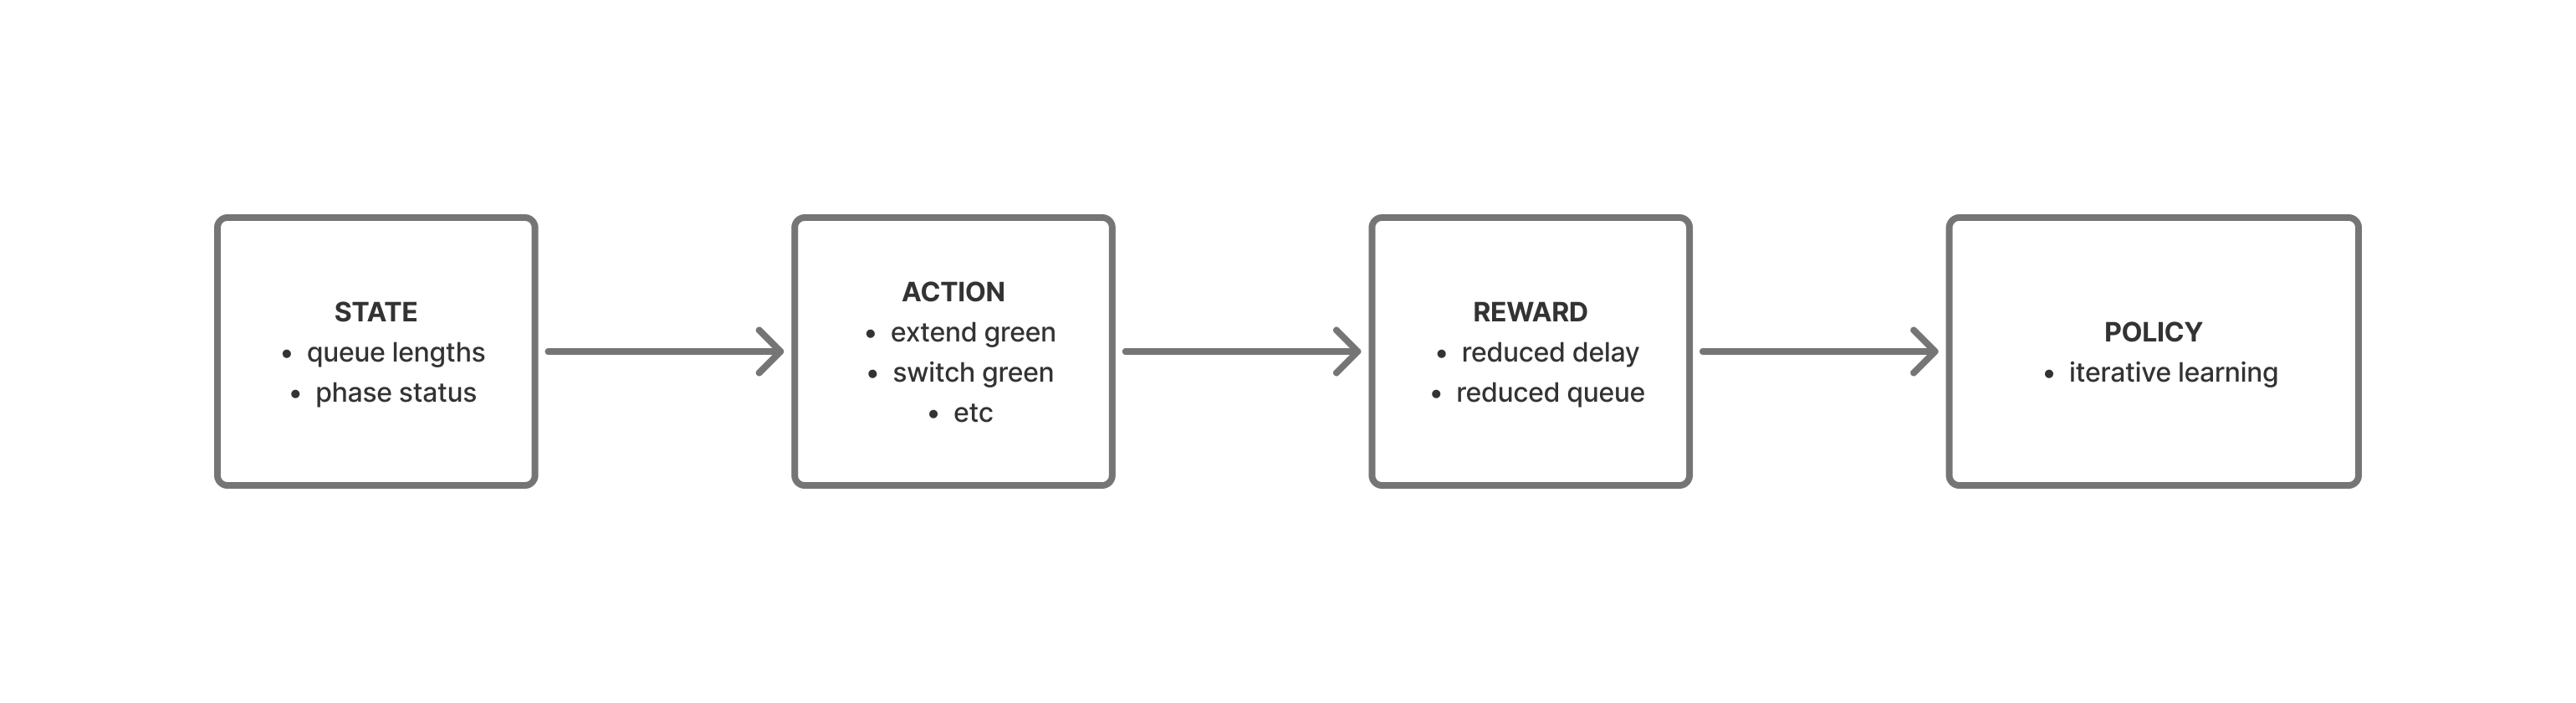
\includegraphics[width=1\linewidth]{Flow chart (Community) (3).png}  
    \caption{Block Diagram of Reinforcement Learning System}
    \label{fig:reinforcement_learning_block}
\end{figure}

\subsection{Reinforcement Learning (RL) Update Rule}

The Q-learning algorithm updates its knowledge of the optimal policy through the following recursive relation:

\begin{equation}
Q(s,a) \leftarrow Q(s,a) + \alpha \big[ r + \gamma \max_{a'} Q(s',a') - Q(s,a) \big]
\label{eq:qlearning}
\end{equation}

where:

\begin{itemize}
    \item $Q(s,a)$ represents the value of taking action $a$ in state $s$
    \item $\alpha$ is the learning rate that controls how much new information overrides old estimates
    \item $\gamma$ is the discount factor determining the importance of future rewards
    \item $r$ is the immediate reward received after taking action $a$
    \item $s'$, $a'$ denote the next state and action
\end{itemize}

This equation enables the learning agent to iteratively improve its policy by updating the estimated value of each state--action pair based on observed rewards. The algorithm updates its knowledge until a point of convergence toward an optimal policy that minimises total traffic delay or maximises throughput whereby its learning rate becomes constant.

Variants such as Deep Q-Networks (DQN), Actor--Critic (A2C, A3C), Proximal Policy Optimization (PPO), and Multi-Agent RL extend this framework to complex, multi-intersection environments.

\subsubsection{Reinforcement Learning Models}

Reinforcement Learning (RL) has emerged as one of the most effective model-free optimisation approaches in traffic signal control. Unlike model based controllers, which rely on fixed mathematical descriptions of traffic flow, RL agents learn control strategies directly through repeated interaction with the environment. This allows an RL controller to adapt to irregular traffic patterns, unforeseen disturbances, and non-linear flow characteristics that conventional models cannot explicitly describe \cite{futuretransp5040137}.

In the RL framework, traffic control is represented as a Markov Decision Process (MDP). At each decision step, the controller observes the current traffic state $s_t$, selects a signal action $a_t$, receives a reward $r_t$ based on system performance, and transitions to a new state $s_{t+1}$. Over time, the agent learns a policy $\pi(a|s)$ that maximises expected cumulative reward. Figure \ref{fig:rl_overall_block} illustrates the high level RL control loop.

\begin{figure}[H]
\centering
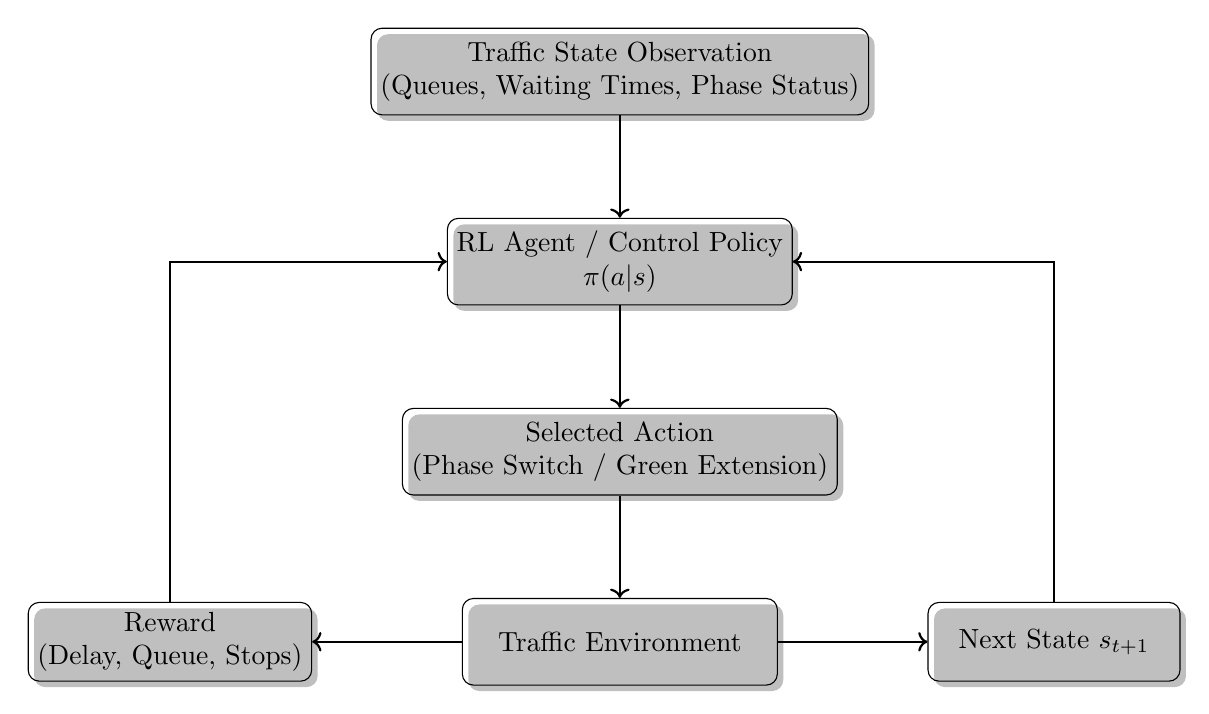
\begin{tikzpicture}[
    node distance=1.3cm,
    block/.style={rectangle, draw, rounded corners, minimum width=4.0cm, minimum height=1.1cm, align=center, drop shadow},
    smallblock/.style={rectangle, draw, rounded corners, minimum width=3.2cm, minimum height=1cm, align=center, drop shadow},
    arrow/.style={->, thick},
]

% Main vertical flow
\node[block] (state) {Traffic State Observation\\(Queues, Waiting Times, Phase Status)};
\node[block, below=of state] (policy) {RL Agent / Control Policy\\$\pi(a|s)$};
\node[block, below=of policy] (action) {Selected Action\\(Phase Switch / Green Extension)};
\node[block, below=of action] (environment) {Traffic Environment};

% Side nodes
\node[smallblock, left=1.9cm of environment] (reward) {Reward\\(Delay, Queue, Stops)};
\node[smallblock, right=1.9cm of environment] (nextstate) {Next State $s_{t+1}$};

% Arrows
\draw[arrow] (state) -- (policy);
\draw[arrow] (policy) -- (action);
\draw[arrow] (action) -- (environment);

\draw[arrow] (environment) -- (reward);
\draw[arrow] (environment) -- (nextstate);

\draw[arrow] (reward) |- (policy);
\draw[arrow] (nextstate) |- (policy);

\end{tikzpicture}
\caption{High-level RL control loop for adaptive traffic signal control.}
\label{fig:rl_overall_block}
\end{figure}

\paragraph{Deep Q-Learning (DQN)}

Deep Q-Learning approximates the action-value function $Q(s,a)$ using a deep neural network rather than a lookup table, which makes it practical for the high-dimensional state spaces that real traffic intersections produce. It applies the same Q-learning update rule (Equation~\ref{eq:qlearning}) but introduces two mechanisms to keep training stable: experience replay, which breaks the temporal correlation between consecutive samples by storing and randomly sampling past transitions; and a target network, a periodic copy of the Q-network whose weights are held fixed for several updates so the learning targets do not shift with every gradient step. Figure \ref{fig:dqn_block} shows the improved systems-engineering diagram for the DQN workflow.

\begin{figure}[H]
\centering
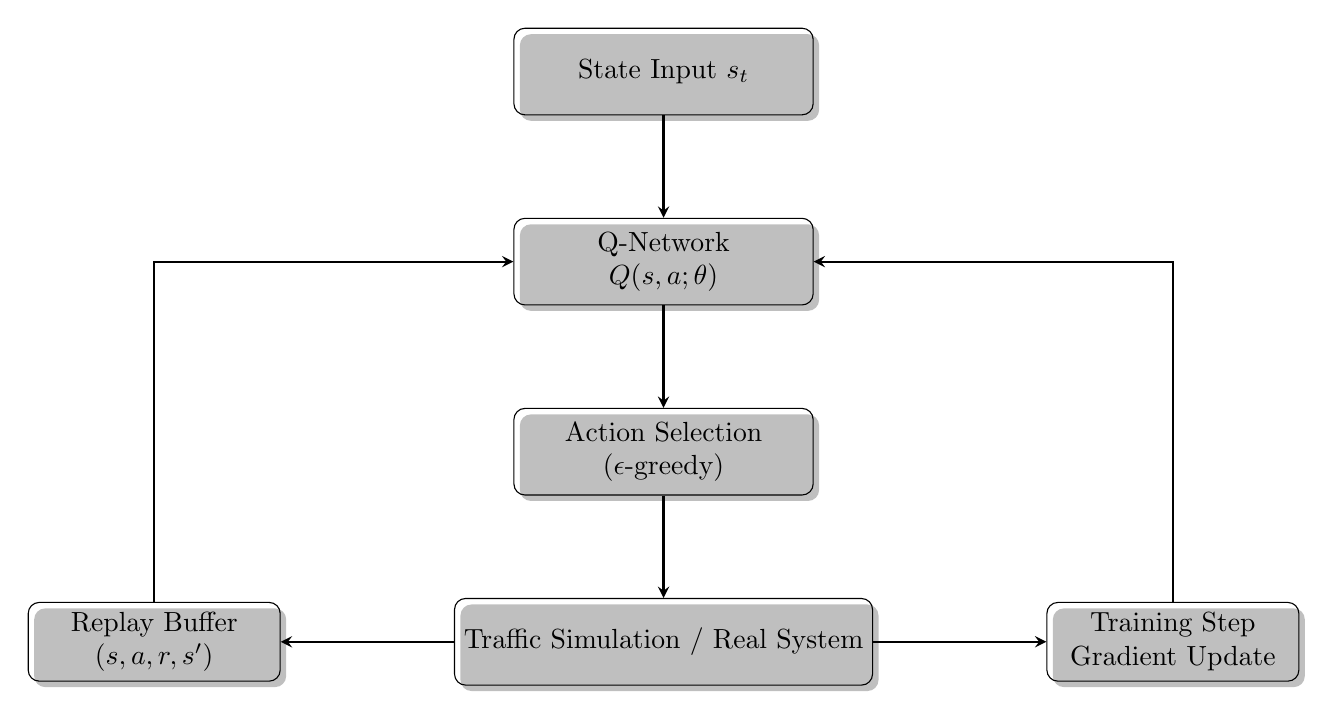
\begin{tikzpicture}[
    node distance=1.3cm,
    block/.style={
        rectangle, draw, rounded corners,
        minimum width=3.8cm, minimum height=1.1cm,
        align=center, drop shadow
    },
    sideblock/.style={
        rectangle, draw, rounded corners,
        minimum width=3.2cm, minimum height=1.0cm,
        align=center, drop shadow
    },
    arrow/.style={-stealth, thick}
]

% Main vertical blocks
\node[block] (state) {State Input $s_t$};
\node[block, below=of state] (qnet) {Q-Network\\$Q(s,a;\theta)$};
\node[block, below=of qnet] (act) {Action Selection\\($\epsilon$-greedy)};
\node[block, below=of act] (env) {Traffic Simulation / Real System};

% Side blocks
\node[sideblock, left=2.2cm of env] (buffer) {Replay Buffer\\$(s,a,r,s')$};
\node[sideblock, right=2.2cm of env] (train) {Training Step\\Gradient Update};

% Main arrows
\draw[arrow] (state) -- (qnet);
\draw[arrow] (qnet) -- (act);
\draw[arrow] (act) -- (env);

% Side arrows
\draw[arrow] (env.west) -- (buffer.east);
\draw[arrow] (buffer.north) |- (qnet.west);

\draw[arrow] (env.east) -- (train.west);
\draw[arrow] (train.north) |- (qnet.east);

\end{tikzpicture}
\caption{DQN architecture for traffic signal decision making.}
\label{fig:dqn_block}
\end{figure}

\paragraph{Proximal Policy Optimization (PPO)}

PPO is an actor--critic method known for its stability and strong performance in continuous and discrete action environments. It updates the policy using a clipped surrogate objective to prevent destructive updates:

\begin{equation}
\mathcal{L}^{\text{CLIP}} = 
\mathbb{E}\left[\min\left(
r_t(\theta)\hat{A}_t,\;\;
\text{clip}(r_t(\theta),1-\epsilon,1+\epsilon)\hat{A}_t
\right)\right]
\label{eq:ppo}
\end{equation}

where $r_t(\theta)=\frac{\pi_{\theta}(a_t|s_t)}{\pi_{\theta_{\text{old}}}(a_t|s_t)}$ is the probability ratio. Figure \ref{fig:ppo_block} shows the PPO system architecture.

\begin{figure}[H]
\centering
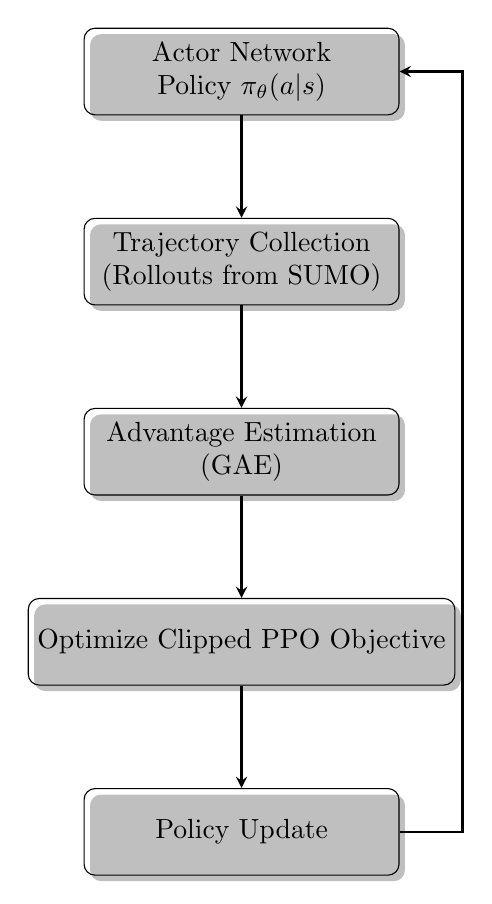
\begin{tikzpicture}[
    node distance=1.3cm,
    block/.style={
        rectangle, draw, rounded corners,
        minimum width=4.0cm, minimum height=1.1cm,
        align=center, drop shadow
    },
    arrow/.style={-stealth, thick},
]

% Main vertical flow
\node[block] (actor) {Actor Network\\Policy $\pi_\theta(a|s)$};
\node[block, below=of actor] (roll) {Trajectory Collection\\(Rollouts from SUMO)};
\node[block, below=of roll] (adv) {Advantage Estimation\\(GAE)};
\node[block, below=of adv] (opt) {Optimize Clipped PPO Objective};
\node[block, below=of opt] (update) {Policy Update};

% Vertical arrows
\draw[arrow] (actor) -- (roll);
\draw[arrow] (roll) -- (adv);
\draw[arrow] (adv) -- (opt);
\draw[arrow] (opt) -- (update);

% Clean loopback arrow
\draw[arrow] (update.east) -| ([xshift=0.8cm]actor.east) -- (actor.east);

\end{tikzpicture}
\caption{Proximal Policy Optimization workflow.}
\label{fig:ppo_block}
\end{figure}

\paragraph{Continuous Control Models DDPG, TD3, SAC}

For green-time allocation where actions are continuous, deterministic or stochastic actor--critic algorithms are used:

\begin{itemize}
    \item DDPG: deterministic signal policy; useful but unstable.
    \item TD3: improves DDPG via clipped double Q-learning.
    \item SAC: adds entropy regularization for robust exploration.
\end{itemize}

These methods allow the agent to choose precise green durations instead of discrete phase selections.

\subsection{Multi-Agent Reinforcement Learning (MARL)}

Multi-Agent Reinforcement Learning extends single-agent RL to settings where multiple autonomous agents act simultaneously within a shared environment. Each agent observes part of the world, selects an action, and receives a reward, but its outcome is influenced by the simultaneous decisions of the other agents. This interdependency is the defining challenge of MARL: what looks like a stationary environment to one agent is in fact being altered by the policies of all others, which can cause individual learning algorithms to oscillate or fail to converge \cite{busoniu2008comprehensive}.

MARL is formalised as a Decentralised Partially Observable Markov Decision Process (Dec-POMDP), in which each agent $i$ receives a local observation $o_i$ drawn from the global state $s$, chooses action $a_i$, and receives a team reward $r$. The joint policy $\boldsymbol{\pi} = \langle \pi_1, \ldots, \pi_n \rangle$ is optimised to maximise cumulative expected return for the group. Applications span robotics, game playing, autonomous vehicles, and networked infrastructure control, anywhere a set of interacting decision-makers must be coordinated without requiring a single central controller \cite{busoniu2008comprehensive}.

When applied to road networks, MARL assigns a separate agent to each signalised intersection. Managing all signals through one joint action space quickly becomes impractical because the action space grows exponentially with every additional junction. MARL keeps the problem tractable while still allowing agents to coordinate across the network by learning joint behaviour through shared experience or explicit communication during training \cite{busoniu2008comprehensive}.

\subsubsection{The centralised decentralised spectrum}

MARL approaches differ mainly in how much information agents share during training and at runtime. At one end, a single controller sees the entire network. At the other, each agent is on its own. Both cause problems.

\paragraph{Fully centralised control}

A centralised controller observes the full network state and outputs a joint action for all intersections. In theory this finds the globally optimal policy, but the joint state and action spaces grow combinatorially with every junction added, so training becomes computationally infeasible beyond a small network \cite{mannion2016experimental}. There is also a deployment problem where all sensor data has to reach one processing unit in real time, which introduces latency and creates a single point of failure.

\paragraph{Fully decentralised control with independent learning}

At the other extreme, every agent treats the rest as just part of the environment and learns purely from its own local observations. The simplest form is Independent Q-Learning (IQL), where each intersection runs a plain DQN. The catch is that all the agents are updating their policies at the same time, so from any single agent's point of view the environment keeps shifting under it. That breaks the Markov assumption Q-learning leans on, and training ends up oscillating or never settling \cite{tan1993multi}. In a traffic network the failure is predictable: independent agents land on strategies that are sensible for one junction but bad for the whole. An intersection will hang onto its green to flush its own queue, dumping those vehicles straight into the next junction and making delay worse network wide..

\subsubsection{Centralised training with decentralised execution (CTDE)}

CTDE, formalised by \cite{oliehoek2008optimal} and made widely known through MADDPG \cite{lowe2017multi}, separates what is needed at training time from what is needed at deployment. The restriction on information sharing only applies when the system is running in the real world. During training, which happens entirely in simulation, agents can share whatever is useful.

Each agent keeps a local policy (the Actor) that takes only its own observations as input. This is what runs on the deployed system. A centralised value function (the Critic) is trained on the full joint state of all agents and is only used during training. Once training ends, the Critic is discarded. Every intersection then runs its Actor on local sensor data alone.

\begin{figure}[H]
\centering
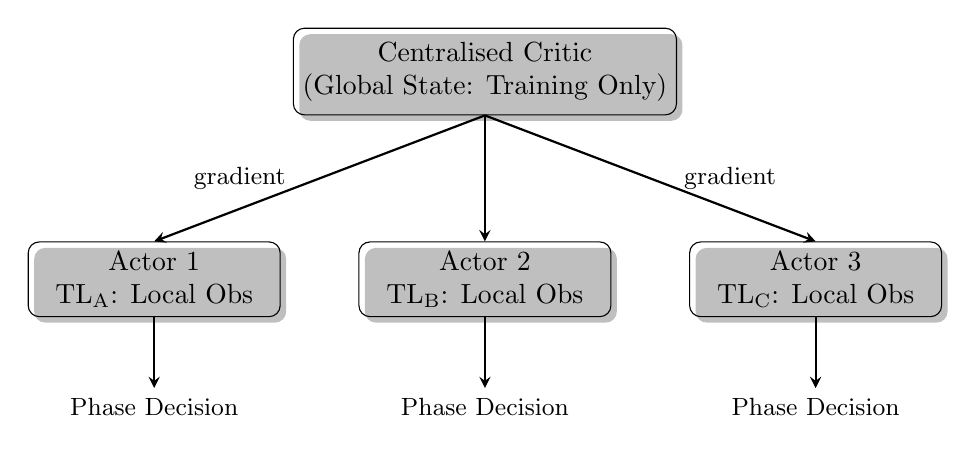
\begin{tikzpicture}[
    node distance=1.1cm,
    block/.style={
        rectangle, draw, rounded corners,
        minimum width=4.5cm, minimum height=1.1cm,
        align=center, drop shadow
    },
    agent/.style={
        rectangle, draw, rounded corners,
        minimum width=3.2cm, minimum height=0.9cm,
        align=center, drop shadow
    },
    arrow/.style={-stealth, thick},
]

\node[block] (critic) {Centralised Critic\\(Global State: Training Only)};

\node[agent, below=1.6cm of critic, xshift=-4.2cm] (a1) {Actor 1\\TL\textsubscript{A}: Local Obs};
\node[agent, below=1.6cm of critic]                (a2) {Actor 2\\TL\textsubscript{B}: Local Obs};
\node[agent, below=1.6cm of critic, xshift= 4.2cm] (a3) {Actor 3\\TL\textsubscript{C}: Local Obs};

\draw[arrow] (critic.south) -- (a1.north) node[midway, left=0.3cm]{\small gradient};
\draw[arrow] (critic.south) -- (a2.north);
\draw[arrow] (critic.south) -- (a3.north) node[midway, right=0.3cm]{\small gradient};

\draw[arrow] (a1.south) -- ++(0,-0.9) node[below]{\small Phase Decision};
\draw[arrow] (a2.south) -- ++(0,-0.9) node[below]{\small Phase Decision};
\draw[arrow] (a3.south) -- ++(0,-0.9) node[below]{\small Phase Decision};

\end{tikzpicture}
\caption{Centralised training with decentralised execution (CTDE).}
\label{fig:ctde_diagram}
\end{figure}

Because the Critic observes all agents at once, it operates in a stationary joint environment, which is what the independent learning approach breaks. Each Actor receives stable gradient signals during training even though it only ever sees its own local data \cite{lowe2017multi}.

\subsubsection{Key CTDE algorithms}

\paragraph{MADDPG}

Lowe et al.\ \cite{lowe2017multi} extended DDPG to the multi-agent setting by giving each agent its own centralised critic conditioned on all agents' observations and actions. It was among the first algorithms to show that CTDE could handle cooperative and competitive tasks in continuous action spaces. It does inherit DDPG's training instability, and maintaining a separate critic per agent becomes expensive as the network grows.

\paragraph{QMIX}

QMIX \cite{rashid2018qmix} decomposes the joint action-value function $Q_{tot}$ into per-agent values $Q_i$ through a mixing network, under a monotonicity constraint:
\begin{equation}
\frac{\partial Q_{tot}}{\partial Q_i} \geq 0 \quad \forall i
\label{eq:qmix_monotone}
\end{equation}
This guarantees that the action each agent picks independently is also the globally optimal joint action, so decentralised execution is safe. QMIX showed strong results on the StarCraft Multi-Agent Challenge \cite{samvelyan2019starcraft} and has been applied to traffic signal control with discrete action spaces.

\paragraph{MAPPO}

Yu et al.\ \cite{yu2022surprising} showed that extending PPO directly to cooperative multi-agent settings (MAPPO) matches or beats more specialised algorithms including QMIX across a range of benchmarks. Each agent has its own Actor on local observations; a single shared Critic takes the concatenated global state of all agents. The PPO clipped objective applies to each agent with a shared advantage estimate:
\begin{equation}
\mathcal{L}^{\text{CLIP}}_i = \mathbb{E}\left[\min\left(r_i(\theta)\hat{A}, \;\text{clip}(r_i(\theta), 1-\epsilon, 1+\epsilon)\hat{A}\right)\right]
\label{eq:mappo_clip}
\end{equation}

where $r_i(\theta) = \frac{\pi_\theta(a_i | o_i)}{\pi_{\theta_\text{old}}(a_i | o_i)}$ is the probability ratio for agent $i$, and $\hat{A}$ is the advantage estimated from the centralised critic via GAE \cite{schulman2015high}. The result from \cite{yu2022surprising} is that PPO's simplicity is not a weakness; a well tuned shared critic with normalised advantages is enough to get strong cooperative performance without the added complexity of value decomposition.

\subsubsection{Parameter sharing}

When all agents observe the same feature types and choose from the same action space, as is the case for a network of similar intersections, they can share Actor network weights. Training uses experience from all agents simultaneously, which multiplies the effective batch size and tends to produce more stable gradients than training separate networks per agent \cite{gupta2017cooperative}. It also reduces the total number of parameters, making training faster.

\subsubsection{Cooperative reward design}
The way the reward is defined goes a long way toward deciding whether agents end up cooperating or competing \cite{chu2019multi}. The literature settles on three options:

\begin{enumerate}
    \item Local reward: each agent is scored only on its own intersection. It is cheap to compute but breeds selfish behaviour, where an agent extends its green to flush its own queue and shoves the overflow into the next junction.
    \item Global reward: every agent shares a single reward computed over the whole network, such as total waiting time. This aims squarely at network-level cooperation, but it makes it harder for any one agent to tell which of its own actions actually moved the number.
    \item Mixed reward: a weighted blend of the two.
\end{enumerate}

Across traffic signal studies, a global reward backed by a centralised critic for credit assignment consistently beats local rewards on network wide outcomes \cite{chu2019multi, wei2019colight}. The critic figures out which global states are worth being in, even when you cannot cleanly separate what each individual agent contributed.
\subsubsection{MARL applied to traffic signal control}

Chu et al \ \cite{chu2019multi} applied multi-agent advantage actor-critic to a 6$\times$6 grid network, where each agent received its local observation plus data from immediate neighbours. Including neighbourhood observations cut average travel time noticeably compared to independent learning.

Wei et al.\ \cite{wei2019colight} developed CoLight using graph attention networks, allowing each intersection to attend selectively to its neighbours' states during training. It achieved leading results on both synthetic and real world datasets. The gap over simpler sharing schemes suggests that how information is structured matters, not just whether agents share at all.

Zheng et al.\ \cite{zheng2019learning} studied a signalised arterial corridor (a linear sequence of intersections along a main road, which is the same layout as the three junctions on the A1 through Palapye). Agents trained with a global reward and CTDE learned phase offsets resembling green wave coordination without being programmed to do so.

\subsubsection{Comparison of MARL algorithms for traffic signal control}

Table~\ref{tab:marl_comparison} summarises the four main MARL algorithms considered for traffic signal control applications, comparing them on the criteria most relevant to a real intersection network: training paradigm, action space compatibility, scalability, and suitability for the Palapye corridor.

\begin{table}[H]
\centering
\caption{Comparison of MARL algorithms for traffic signal control}
\label{tab:marl_comparison}
\begin{tabular}{p{2.0cm}p{2.6cm}p{2.6cm}p{2.6cm}p{2.6cm}}
\toprule
\textbf{Algorithm} & \textbf{Training paradigm} & \textbf{Action space} & \textbf{Key limitation} & \textbf{Relevance to Palapye} \\
\midrule
IQL & Fully decentralised & Discrete & Non-stationary training; agents ignore each other & Weak: no corridor coordination \\
MADDPG & CTDE, separate critics & Continuous & Unstable with many agents; requires continuous actions & Partial: corridor-aware but poor fit for discrete phases \\
QMIX & CTDE, value decomposition & Discrete & Monotonicity constraint limits expressivity & Good: cooperative, discrete; more complex than needed \\
MAPPO & CTDE, centralised critic & Discrete & Requires joint state during training & Best fit: cooperative, discrete, proven on similar networks \\
\bottomrule
\end{tabular}
\end{table}

\subsubsection{Algorithm selection: MAPPO for the Palapye network}

MAPPO with parameter sharing and a global cooperative reward was selected for this project. The three Palapye intersections observe the same feature types and choose from the same three green phases, so parameter sharing applies without modification. The discrete action space suits PPO's categorical policy distribution better than continuous-action methods like MADDPG, which have known stability issues. Yu et al.\ \cite{yu2022surprising} showed MAPPO achieves strong cooperative performance without QMIX's value decomposition overhead. A global reward trains the agents to reduce network wide waiting time rather than each junction optimising itself at the expense of the others.

\section{Summary Comparison of Control Approaches}

Table~\ref{tab:lit_review_summary} provides a consolidated comparison of the control strategies reviewed in this chapter, evaluated against the criteria most relevant to the Palapye A1 corridor: data requirements, real time adaptability, multi-intersection scalability, and suitability for deployment in a data scarce environment.

\begin{table}[H]
\centering
\caption{Comparison of traffic signal control approaches reviewed in Chapter 2}
\label{tab:lit_review_summary}
\begin{tabular}{p{2.2cm}p{2.0cm}p{1.8cm}p{2.0cm}p{1.6cm}p{2.8cm}}
\toprule
\textbf{Method} & \textbf{Required data} & \textbf{Real time adaptive} & \textbf{Multi-inter-section} & \textbf{Scalable} & \textbf{Limitation for Palapye} \\
\midrule
Fixed-time & Historical counts & No & Via coordination & Yes & No response to demand variation \\
Actuated & Live loop/camera & Partial & Limited & Moderate & No predictive or cooperative capability \\
MPC & Accurate model & Yes & Hierarchical & Low & High compute; model accuracy required \\
DTA & Network-wide OD & Partial & Yes & Low & Routing focus, not signal timing \\
MILP & Full network data & No (offline) & Yes & Very low & Computationally intractable online \\
Q-learning & Simulation & Yes & Partial & Low & Tabular; cannot scale to continuous state \\
DQN & Simulation & Yes & Partial & Moderate & Unstable with many agents \\
SA-PPO & Simulation & Yes & No & Moderate & Single junction only; no coordination \\
MAPPO & Simulation & Yes & Yes (CTDE) & Good & Joint state required during training \\
\bottomrule
\multicolumn{6}{l}{\footnotesize CTDE = Centralised Training, Decentralised Execution; OD = origin--destination; SA = single-agent.}
\end{tabular}
\end{table}

MAPPO is selected on this basis. It is the only approach that combines real-time adaptability, multi-intersection coordination, and a discrete action space compatible with phase-based signal control, without requiring historical traffic data or an accurate traffic model.

\chapter{Methodology}

\section{Overview of the Methodology}

The implemented traffic signal optimisation system follows a two-phase methodology that progressively scales from a single-intersection baseline to a three-intersection multi-agent corridor controller. Both phases are grounded in Deep Reinforcement Learning (DRL) and use the Simulation of Urban Mobility (SUMO) environment as the evaluation platform.

\textbf{Phase 1: Single-Agent Baseline (Chapters 3--5).} The first phase constructed a SUMO network modelling one signalised intersection, generated synthetic traffic data across demand scenarios, and trained a single Proximal Policy Optimisation (PPO) agent using Stable-Baselines3. A YOLOv8-based CameraVision module was developed and validated independently on sample Palapye traffic footage, demonstrating the feasibility of camera based queue estimation and providing a pathway toward real world sensor integration. The Phase 1 evaluation compared the PPO controller quantitatively against a fixed time baseline.

\textbf{Phase 2: Multi-Agent Extension (Chapters 6--7).} The second phase extended the network to all three signalised junctions along the A1 Palapye corridor and replaced the single-agent controller with a cooperative Multi-Agent PPO (MAPPO) system. A custom PettingZoo parallel environment was implemented with three agents under Centralised Training, Decentralised Execution, a shared cooperative reward signal, green wave pre-computation, and a three-stage curriculum over six demand scenarios. The Phase 2 evaluation compared MAPPO against both the fixed time baseline and the Phase 1 single-agent PPO baseline.

The workflow below explores the following major components:

\begin{itemize}
    \item SUMO network construction 
    \item SUMO based environment generation and RL interaction for policy learning via TraCI
    \item YOLOv8 vehicle detection and queue estimation, which is tested independently.
    \item Single-agent PPO controller training and evaluation (Phase 1)
    \item MAPPO multi-agent controller design, training, and evaluation (Phase 2)
\end{itemize}

Python libraries including PyTorch, PettingZoo, OpenCV, and Stable-Baselines3 were used across the two phases. The TraCI interface links SUMO with Python in real time for both training and evaluation.

Figure~\ref{fig:methodology_overview} shows the high level flow of the Phase 1 methodology from network construction through to policy evaluation.

\begin{figure}[H]
\centering
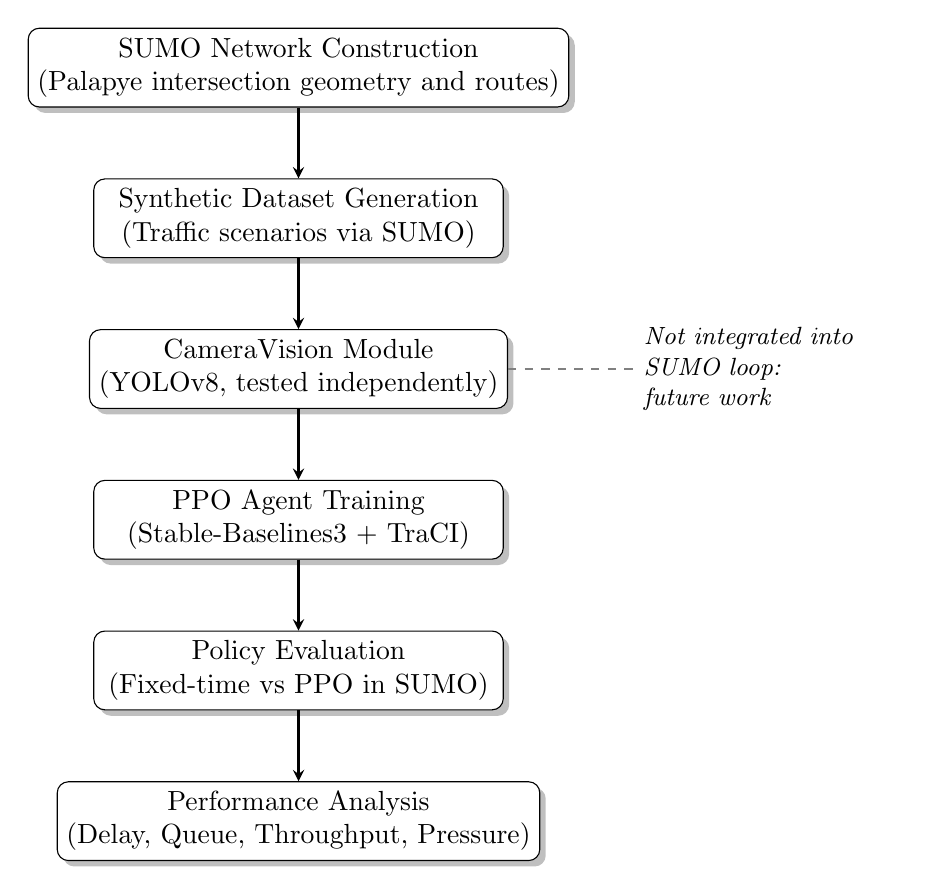
\begin{tikzpicture}[
    node distance=0.9cm,
    block/.style={rectangle, draw, rounded corners, minimum width=5.2cm, minimum height=1.0cm, align=center, drop shadow, fill=white},
    decision/.style={diamond, draw, minimum width=3.2cm, minimum height=0.9cm, align=center, drop shadow, fill=white, aspect=2.5},
    arrow/.style={-stealth, thick},
]

\node[block] (net)    {SUMO Network Construction\\(Palapye intersection geometry and routes)};
\node[block, below=of net]  (data)   {Synthetic Dataset Generation\\(Traffic scenarios via SUMO)};
\node[block, below=of data] (cam)    {CameraVision Module\\(YOLOv8, tested independently)};
\node[block, below=of cam]  (train)  {PPO Agent Training\\(Stable-Baselines3 + TraCI)};
\node[block, below=of train](eval)   {Policy Evaluation\\(Fixed-time vs PPO in SUMO)};
\node[block, below=of eval] (result) {Performance Analysis\\(Delay, Queue, Throughput, Pressure)};

\draw[arrow] (net)    -- (data);
\draw[arrow] (data)   -- (cam);
\draw[arrow] (cam)    -- (train);
\draw[arrow] (train)  -- (eval);
\draw[arrow] (eval)   -- (result);

% Side note for CameraVision
\node[right=1.6cm of cam, align=left, text width=3.2cm, font=\small\itshape]
    (sidenote) {Not integrated into\\SUMO loop:\\future work};
\draw[dashed, gray] (cam.east) -- (sidenote.west);

\end{tikzpicture}
\caption{High-level methodology flow from network construction to performance evaluation.}
\label{fig:methodology_overview}
\end{figure}



\section{System Architecture and Dashboard Design}

The implemented architecture is composed of the following components:

\begin{itemize}
    \item SUMO Environment Module (RL interaction via state action reward cycles)
    \item Real-Time Data Collection Module (CameraVision + YOLO testing)
    \item Model Control Module (Proximal Policy Optimisation Agent)
\end{itemize}

During simulation the modules run as a semi-closed loop: SUMO generates traffic, the DRL agent picks an action, and SUMO advances the traffic state from there. CameraVision was tested on its own; full integration into the closed loop is left as future work. Figure~\ref{fig:system_arch} shows how the three modules connect.
\begin{figure}[H]
\centering
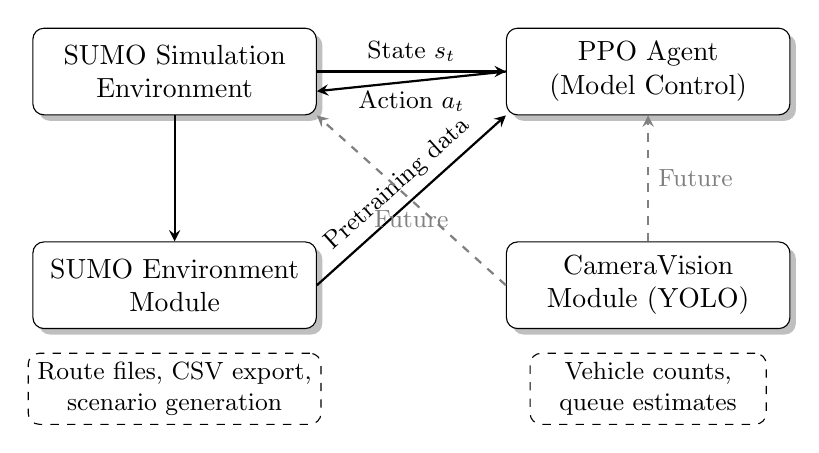
\begin{tikzpicture}[
    node distance=1.1cm and 1.8cm,
    block/.style={rectangle, draw, rounded corners, minimum width=3.6cm, minimum height=1.1cm, align=center, drop shadow, fill=white},
    subblock/.style={rectangle, draw, dashed, rounded corners, minimum width=3.0cm, minimum height=0.85cm, align=center, fill=white, font=\small},
    arrow/.style={-stealth, thick},
    dasharrow/.style={-stealth, thick, dashed, gray},
]

% Top-level modules
\node[block] (sumo)  {SUMO Simulation\\Environment};
\node[block, right=2.4cm of sumo] (ppo) {PPO Agent\\(Model Control)};
\node[block, below=1.6cm of sumo] (data) {SUMO Environment\\Module};
\node[block, below=1.6cm of ppo]  (cam)  {CameraVision\\Module (YOLO)};

% Sub-labels
\node[subblock, below=0.3cm of data] (sumodata) {Route files, CSV export,\\scenario generation};
\node[subblock, below=0.3cm of cam]  (camdata)  {Vehicle counts,\\queue estimates};

% Arrows: SUMO <-> PPO (closed loop)
\draw[arrow] (sumo.east) -- node[above, font=\small]{State $s_t$} (ppo.west);
\draw[arrow] (ppo.west)  -- node[below, font=\small]{Action $a_t$} ([yshift=-0.25cm]sumo.east);

% Arrows: Dataset module feeds into PPO pretraining
\draw[arrow] (data.east) -- node[above, font=\small, sloped]{Pretraining data} (ppo.south west);

% Dashed: CameraVision (future integration)
\draw[dasharrow] (cam.north) -- node[right, font=\small]{Future} (ppo.south);
\draw[dasharrow] (cam.west)  -- node[below, font=\small]{Future} (sumo.south east);

% Data flows
\draw[arrow] (sumo.south) -- (data.north);

\end{tikzpicture}
\caption{System architecture and data flows across the three modules.}
\label{fig:system_arch}
\end{figure}

A system dashboard was also implemented to visualise:

\begin{itemize}
    \item Detected vehicles (YOLO test visualisation)
    \item Queue lengths per approach
    \item Active signal phase
    \item Reinforcement learning agent actions in real time.
\end{itemize}
\subsection{SUMO Based Environment Generation and RL Interaction}

The PPO and MAPPO agents here do not learn from a static dataset the way a supervised model would. They learn by interacting with the SUMO simulation: at each timestep the agent reads the current traffic state, picks a phase action, gets back a reward, and uses that experience to update its policy. SUMO is the environment the agent acts in, not a pile of data it reads from.

\paragraph{Absence of Real Historical Data}

There were no public historical datasets for the Palapye A1 intersections to begin with. Neither the local authorities nor any online repository had usable records of traffic volumes, waiting times, or past signal timings. That is in line with the wider data scarcity across sub-Saharan African urban transport, and it is the reason this project trains and evaluates on a synthetically parameterised simulation rather than recorded data.

\paragraph{Synthetic Environment Parameterisation}

The SUMO environment was set up using realistic assumptions for the A1 corridor. Traffic is injected through route files that specify:

\begin{itemize}
    \item Arrival rates per approach (vehicles per second, derived from typical urban arterial volumes)
    \item Vehicle type distributions (cars, motorcycles, trucks, buses) with corresponding SUMO vehicle type definitions
    \item Turning movement probabilities at each junction, estimated from the road geometry and connectivity
    \item Six named demand scenarios spanning the expected operating range: \texttt{low}, \texttt{normal}, \texttt{rush\_hour\_am}, \texttt{rush\_hour\_pm}, \texttt{holiday}, and \texttt{incident}
\end{itemize}

Every training episode draws one demand scenario, runs for a fixed number of environment steps, and hands the accumulated reward back to the policy optimiser. The agent never sees a pre-collected traffic record. Everything it learns comes from the state, action, reward, and next-state transitions the simulation generates as it runs.

\paragraph{SUMO Scenario Generation}

The demand conditions were built as custom SUMO route files, each one a different operating period with its own realistic arrival rates:

\begin{itemize}
    \item \textbf{Low demand} : off-peak conditions with sparse vehicle arrivals across all approaches
    \item \textbf{Normal demand}: typical midday flow with moderate, balanced arrivals
    \item \textbf{Morning rush hour} : high southbound and eastbound inflows representing the morning commute toward Gaborone and BIUST
    \item \textbf{Evening rush hour}: high northbound and westbound inflows representing the return commute
    \item \textbf{Holiday transit}: elevated through traffic on the A1 corridor with reduced turning movements
    \item \textbf{Incident} : asymmetric demand caused by lane reduction or diversion on one approach
\end{itemize}

The route files set the arrival rates, randomise the vehicle types (cars, motorcycles, heavy vehicles), and feed traffic in through multi-lane approaches. Each evaluation episode runs for 1,800 simulation seconds, long enough for queues to build up and clear again over several signal cycles.

\begin{figure}[h]
\centering
 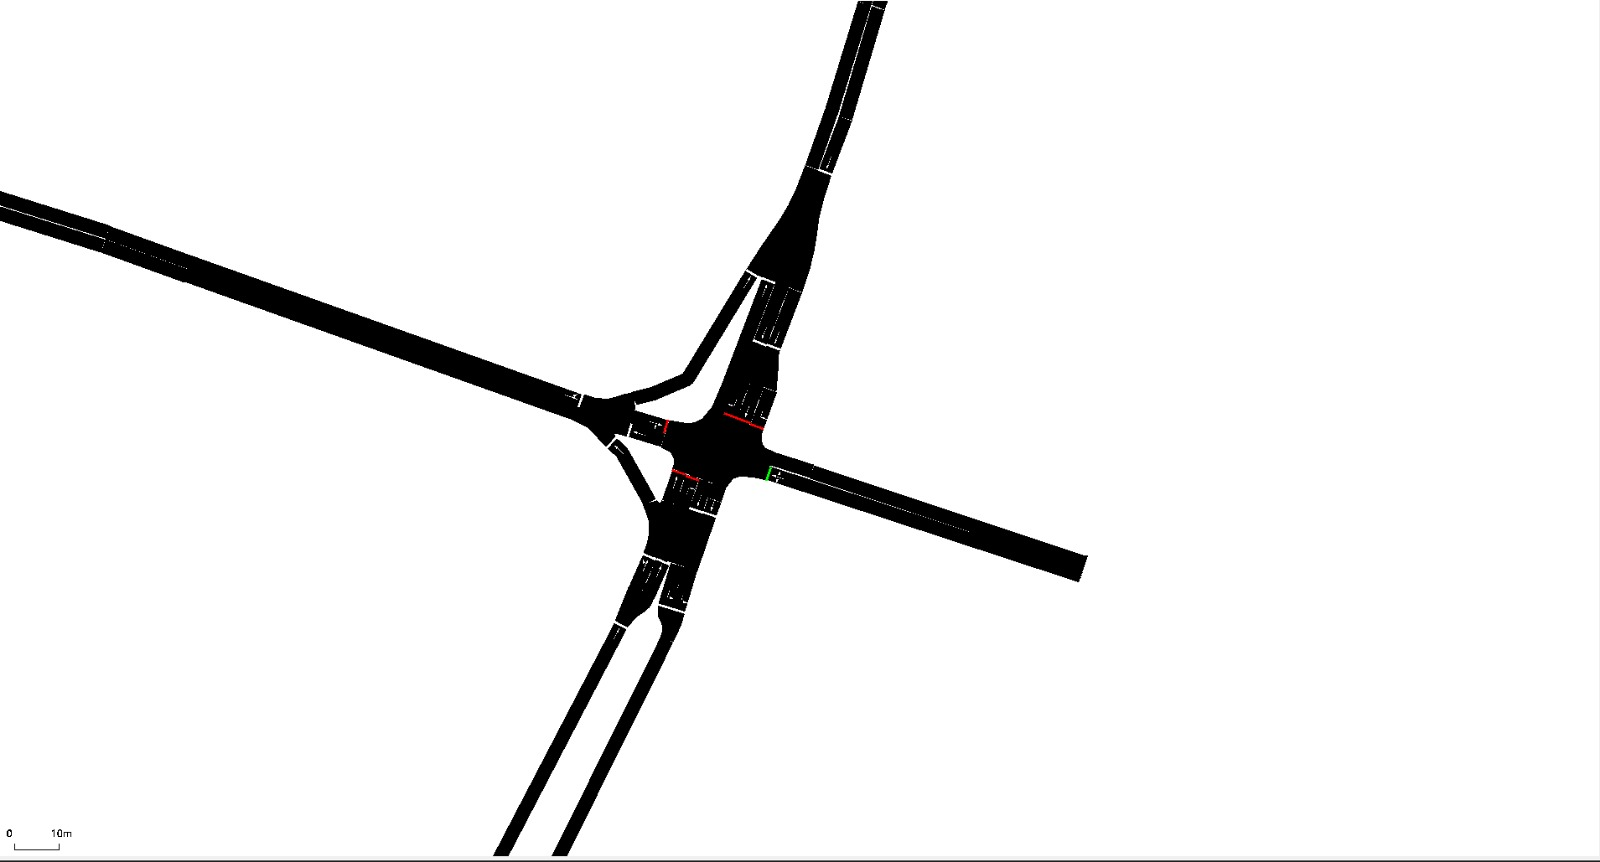
\includegraphics[width=0.9\linewidth]{sumo.jpeg} 
\caption{Custom SUMO intersection used for dataset generation and DRL training.}
\label{fig:sumo_network}
\end{figure}

\subsection{Real-Time Data Collection}

A YOLO based CameraVision module was developed and tested to verify its ability to extract real time traffic metrics from video footage.

\paragraph{CameraVision System}

The CameraVision system processed sample traffic video frames using OpenCV and YOLOv8 to detect and classify vehicles. Extracted metrics included:

\begin{itemize}
    \item Vehicle counts per lane
    \item Queue length estimation
    \item Average lane speeds
    \item Halting information (vehicles $<0.3$ \si{m/s})
    \item Southbound only filtering (direction based detection)
\end{itemize}

\begin{figure}[h]
\centering
 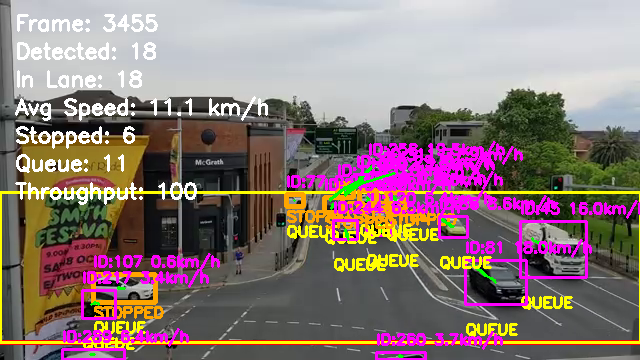
\includegraphics[width=0.9\linewidth]{Traffic Tracker_screenshot_21.11.2025 (another copy).png} 
\caption{YOLOv8 vehicle detection test on sample traffic footage.}
\label{fig:yolo_detection}
\end{figure}

Although functionally successful, this module was not integrated into the SUMO control loop. The YOLOv8 detection pipeline was independently validated on sample footage; full closed loop integration is identified as future work.

\paragraph{Directional Tracking}

Centroid tracking and optical-flow estimation were tested to determine the direction of vehicle travel, enhancing detection accuracy for incoming traffic.

\paragraph{Frame-to-Simulation Synchronisation}

Although full frame-to-SUMO synchronisation was not implemented, a design utilising Python deque structures was prepared for future integration.

\subsection{Model Control}

The decision making component of the system is a Deep Reinforcement Learning (DRL) agent implemented using the Proximal Policy Optimisation (PPO) algorithm. The Model Control module serves as the core logic responsible for determining the most efficient traffic signal phase at any given time, based on continuous feedback from the SUMO simulation environment. This section provides a detailed description of the agent's observation space, action space, reward formulation, and communication with the SUMO environment via TraCI.

\paragraph{Observation Space}

The observation space defines the full set of environmental variables that the agent uses to understand the current state of the intersection. The PPO agent receives a numerical state vector composed of:

\begin{itemize}
    \item \textbf{Queue lengths per lane:} The number of vehicles waiting in each incoming lane.
    \item \textbf{Number of halted vehicles:} Vehicles with a speed less than 0.1 m/s, indicating congestion.
    \item \textbf{Vehicle arrival rate:} The number of vehicles entering each approach within a defined time window.
    \item \textbf{Current signal phase:} Encoded as an integer representing the active traffic light configuration.
    \item \textbf{Average approach speeds:} The mean speed of vehicles across each lane group, used to estimate traffic flow efficiency.
    \item \textbf{Pressure metric:} A traffic control metric defined as $P = \sum(\text{incoming vehicles}) - \sum(\text{outgoing vehicles})$, which represents the directional traffic load at the intersection.
\end{itemize}

These variables collectively allow the DRL agent to maintain an accurate representation of traffic conditions and make informed control decisions.

\paragraph{Action Space}

The action space consists of discrete actions representing all allowed traffic signal phases at the intersection. Each action corresponds to a valid configuration of green, yellow, and red signals. To ensure safety and realism, several constraints are incorporated:

\begin{itemize}
    \item \textbf{Mandatory yellow transition:} Before any phase change, a yellow phase of fixed duration is enforced.
    \item \textbf{Minimum green time:} Each green phase must remain active for a minimum duration to prevent rapid flickering and ensure predictable driver behavior.
    \item \textbf{Prevention of rapid toggling:} The agent is restricted from switching repeatedly between two phases within a short time interval.
\end{itemize}

These constraints prevent unrealistic or unsafe signal sequences while allowing the agent to optimise phase transitions dynamically.

\paragraph{Reward Function}

The reward function is designed to guide the agent toward traffic-efficient behaviour. It combines multiple weighted components that penalise congestion and reward improved traffic movement:

\begin{itemize}
    \item \textbf{Queue penalty:} A negative reward proportional to total queue length across all lanes.
    \item \textbf{Throughput reward:} A positive reward for each vehicle that successfully exits the intersection.
    \item \textbf{Halting penalty:} Additional penalties applied when large numbers of vehicles remain stationary.
    \item \textbf{Phase switching penalty:} Discourages unnecessary signal switching to promote smooth traffic flow.
    \item \textbf{Pressure reduction reward:} Encourages the agent to reduce traffic pressure by prioritising heavily congested approaches.
\end{itemize}

The reward formulation balances local delay reduction, global flow improvement, and controller stability.

\paragraph{SUMO--DRL Interaction via TraCI}

The PPO agent interacts with the SUMO simulation using the TraCI (Traffic Control Interface) protocol. The process occurs in a closed loop:

\begin{enumerate}
    \item \textbf{Action selection:} The agent chooses a phase based on the current observation vector.
    \item \textbf{Traffic light update:} TraCI applies the selected signal phase to the intersection.
    \item \textbf{Simulation advancement:} SUMO advances the simulation by a fixed number of timesteps (e.g., 1--5 seconds) to allow vehicles to react to the new signal.
    \item \textbf{State extraction:} Updated traffic data (queues, speeds, counts) are retrieved from SUMO.
    \item \textbf{Reward calculation:} The environment computes the reward for the previous action.
    \item \textbf{Environment transition:} The next state and reward are returned to the agent for learning and policy improvement.
\end{enumerate}

This closed loop cycle continues for the duration of each episode, enabling the agent to iteratively refine its traffic signal control policy based on observed outcomes and accumulated rewards. Figure~\ref{fig:traci_loop} shows the interaction cycle as a flowchart.

\begin{figure}[H]
\centering
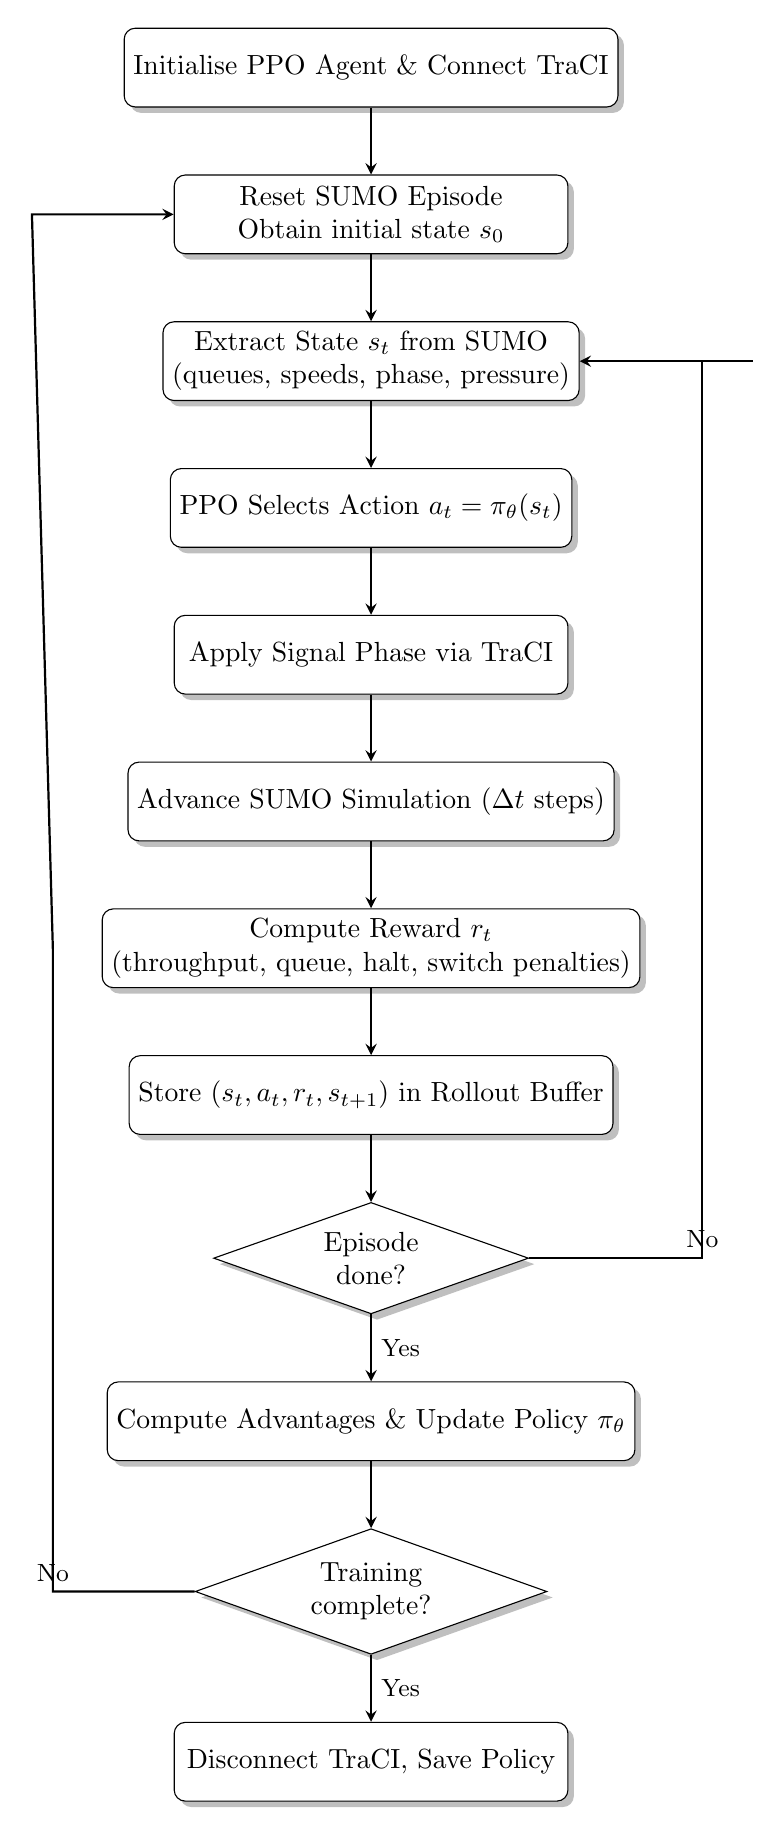
\begin{tikzpicture}[
    node distance=0.85cm,
    block/.style={rectangle, draw, rounded corners, minimum width=5.0cm, minimum height=1.0cm, align=center, drop shadow, fill=white},
    decision/.style={diamond, draw, aspect=2.8, minimum width=4.0cm, minimum height=0.9cm, align=center, drop shadow, fill=white},
    arrow/.style={-stealth, thick},
]

\node[block]    (init)   {Initialise PPO Agent \& Connect TraCI};
\node[block,    below=of init]   (reset)  {Reset SUMO Episode\\Obtain initial state $s_0$};
\node[block,    below=of reset]  (obs)    {Extract State $s_t$ from SUMO\\(queues, speeds, phase, pressure)};
\node[block,    below=of obs]    (act)    {PPO Selects Action $a_t = \pi_\theta(s_t)$};
\node[block,    below=of act]    (apply)  {Apply Signal Phase via TraCI};
\node[block,    below=of apply]  (step)   {Advance SUMO Simulation ($\Delta t$ steps)};
\node[block,    below=of step]   (reward) {Compute Reward $r_t$\\(throughput, queue, halt, switch penalties)};
\node[block,    below=of reward] (store)  {Store $(s_t, a_t, r_t, s_{t+1})$ in Rollout Buffer};
\node[decision, below=of store]  (done)   {Episode\\done?};
\node[block,    below=of done]   (update) {Compute Advantages \& Update Policy $\pi_\theta$};
\node[decision, below=of update] (conv)   {Training\\complete?};
\node[block,    below=of conv]   (end)    {Disconnect TraCI, Save Policy};

% Vertical flow
\draw[arrow] (init)   -- (reset);
\draw[arrow] (reset)  -- (obs);
\draw[arrow] (obs)    -- (act);
\draw[arrow] (act)    -- (apply);
\draw[arrow] (apply)  -- (step);
\draw[arrow] (step)   -- (reward);
\draw[arrow] (reward) -- (store);
\draw[arrow] (store)  -- (done);
\draw[arrow] (done)   -- node[right]{\small Yes} (update);
\draw[arrow] (update) -- (conv);
\draw[arrow] (conv)   -- node[right]{\small Yes} (end);

% Loop back: episode not done -> back to obs
\draw[arrow] (done.east) -- ++(2.2,0) node[above, font=\small]{No}
    |- ([xshift=2.2cm]obs.east) -- (obs.east);

% Loop back: training not complete -> new episode
\draw[arrow] (conv.west) -- ++(-1.8,0) node[above, font=\small]{No}
    -- ++(0,8.15) -- ([xshift=-1.8cm]reset.west) -- (reset.west);

\end{tikzpicture}
\caption{PPO--SUMO closed loop training flowchart via TraCI.}
\label{fig:traci_loop}
\end{figure}

\begin{algorithm}[H]
\caption{PPO Based Traffic Signal Control in SUMO}
\DontPrintSemicolon

Initialize PPO agent with policy network $\pi_\theta$ and value network $V_\phi$\;
Load SUMO network, routes, and traffic light configuration\;
Connect to SUMO using TraCI\;
Set simulation time $t \leftarrow 0$\;

\While{training not complete}{
    
    Reset SUMO episode\;
    Obtain initial traffic state $s_0$ from TraCI\;

    \For{each timestep $t = 0$ \KwTo $T$}{
        
        Extract traffic state variables:\;
        \Indp
            queue lengths, halted vehicles, arrival rates\;
            current signal phase, average speeds\;
            pressure metric (incoming $-$ outgoing)\;
        \Indm
        
        Select action $a_t = \pi_{\theta}(s_t)$\;
        Apply selected signal phase via TraCI\;

        Advance SUMO simulation for $\Delta t$ steps\;

        Retrieve next state $s_{t+1}$ from TraCI\;

        Compute reward $r_t$:\;
        \Indp
            $r_t =$ throughput reward\;
            $r_t \leftarrow r_t -$ queue penalty\;
            $r_t \leftarrow r_t -$ halting penalty\;
            $r_t \leftarrow r_t -$ switching penalty\;
        \Indm

        Store transition $(s_t, a_t, r_t, s_{t+1})$ in rollout buffer\;

        \If{episode terminated}{
            break\;
        }
    }
    
    Compute advantages $\hat{A}_t$, clipped policy loss, value loss, and entropy bonus\;
    Update policy network $\theta$ and value network $\phi$\;

}

Disconnect from TraCI and stop SUMO\;

\end{algorithm}

\section{Assumptions and Scope Boundaries}

The results reported in this dissertation rest on a set of explicit assumptions and deliberate scope boundaries. These are declared here, before any results are presented, so that the validity and generalisability of the findings can be assessed against them. Three assumptions are load-bearing and are highlighted accordingly.

\begin{enumerate}
    \item \textbf{Synthetic traffic demand (load-bearing).} No historical traffic data exist for the Palapye A1 intersections (see the discussion of the absence of real historical data in the Methodology). All demand is synthetically parameterised from typical urban-arterial volumes and road geometry. Consequently, the \emph{direction} and \emph{mechanism} of the reported improvements are defensible, but their absolute \emph{magnitude} is relative to a synthetic baseline and is not validated against measured field data.

    \item \textbf{No pedestrian traffic (load-bearing).} The simulation models vehicle flows only. No pedestrian demand, pedestrian crossing phases, or minimum walk-time constraints are included in the observation, action, or reward design. Real signalised junctions must reserve green time for pedestrian crossings, which would cap the throughput gains achievable by the learned policy. The reported waiting-time reductions are therefore an upper bound relative to a deployment that must service pedestrians.

    \item \textbf{Single training seed (load-bearing).} All learned policies are obtained from a single random seed (\texttt{seed = 42}). Variance across seeds is not characterised, so confidence intervals on policy quality cannot be reported. Multi-seed evaluation is identified as future work.

    \item \textbf{SUMO as a sufficient proxy.} The SUMO micro-simulator is assumed adequate for both training and evaluation. Sensor noise, controller and communication latency, weather, and other real world disturbances are not modelled.

    \item \textbf{Default driver behaviour.} Vehicles follow SUMO's default car following and lane changing models. These are not recalibrated to local driving behaviour.

    \item \textbf{Network geometry.} The three-junction corridor, the inter-junction spacing of approximately 350\,m, and the free-flow speed of approximately 50\,km/h are nominal approximations of the real A1 network used to model the control problem and to initialise the green-wave offsets.

    \item \textbf{Discrete three-phase control.} Each junction is controlled with three green phases (north--south through, east--west through, protected/secondary). Separate turn arrows, all-red clearance, and other phase configurations are out of scope. The fixed timing constants (15\,s minimum green, 6\,s yellow, 75\,s maximum green, 3\,s decision step) are design choices rather than optimised values.

    \item \textbf{Centralised Training, Decentralised Execution (CTDE).} The centralised critic is assumed to have access to the joint network state during offline training only; at execution each agent acts on its 22-dimension local observation alone, with coordination emerging through the shared reward and downstream-occupancy signal rather than explicit inter-agent communication.

    \item \textbf{Homogeneous vehicle priority.} No public-transport priority, emergency-vehicle pre emption, or non motorised traffic (cyclists) is modelled; all vehicles are treated with equal priority.

    \item \textbf{CameraVision as a future pathway.} The YOLOv8 detection module is validated independently and is \emph{not} part of the control loop. The real world deployment pathway assumes that camera based queue estimation can later supply the same observation vector at acceptable accuracy and latency; this integration is untested in this work.
\end{enumerate}

The deeper consequences of these boundaries for the interpretation of specific results are revisited in the Phase~1 ``Limitations and Observations'' section and the Phase~1 baseline limitations discussion.

\chapter{Single Intersection PPO Results and Analysis}

This chapter presents the  results obtained from testing the fixed time traffic signal controller and the proposed PPO based adaptive controller in the SUMO simulation environment. The analysis includes visual evidence of simulation execution, performance metric comparison, and detailed interpretation of system behaviour.

\section{Simulation Setup}

The SUMO simulation interface was configured using the custom intersection network developed in Chapter 3. Both controllers were tested under identical traffic conditions, route files, and simulation durations to ensure fair comparison.

\begin{itemize}
    \item \textbf{Simulation tool:} SUMO-gui
    \item \textbf{Control systems tested:} Fixed-time controller vs PPO agent.
    \item \textbf{Simulation duration:} 300 seconds (5 minutes) for both controllers.
    \item \textbf{Traffic demand:} Identical route flows for both experiments.
    \item \textbf{Performance metrics recorded:} delay, queue length, throughput, stop ratio, and pressure.
    \item \textbf{Evaluation period:} 9,000 simulation timesteps
\end{itemize}

\section{PPO Training Progress}

Before assessing at how the controller performs, we first need to be sure the PPO agent actually learned something during training rather than settling on noise. This section walks through the diagnostic metrics TensorBoard logged over 600,000 training timesteps. Together they confirm the agent converged to a stable policy well before evaluation started.

\subsection{Evaluation Mean Reward}

\begin{figure}[H]
\centering
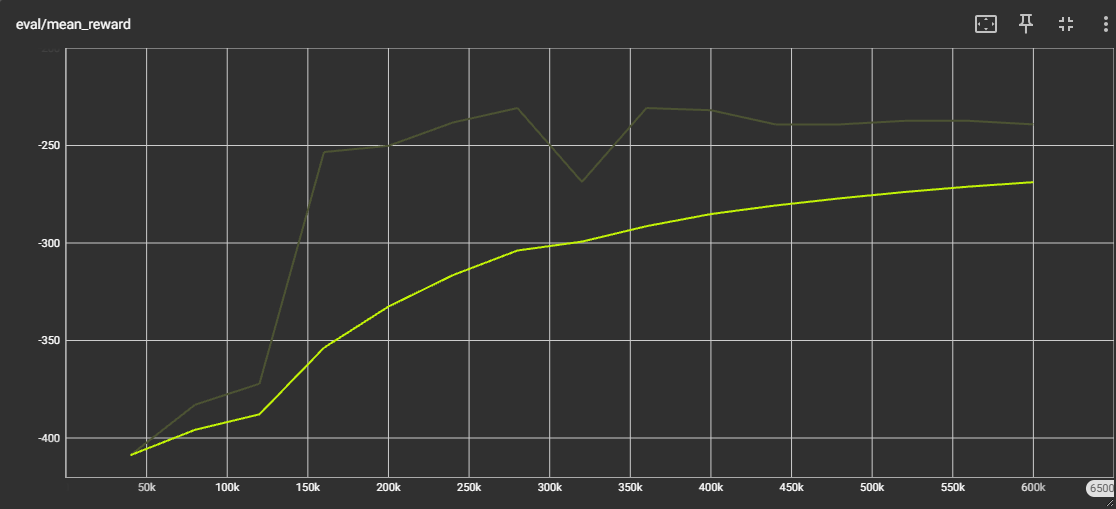
\includegraphics[width=0.95\linewidth]{ppo_eval_reward_smooth.png}
\caption{Smoothed evaluation mean reward over training.}
\label{fig:tb_eval_rew}
\end{figure}

Figure~\ref{fig:tb_eval_rew} shows the deterministic evaluation reward measured periodically throughout training by running the learnt policy greedily against a heldout simulation episode.
The curve shows three phases. The reward climbs fast from $-$390 to $-$255 over the first 150k steps as the agent explores, then refines up to about $-$230 by 250k, a 41\% cut in the combined queue, pressure, and waiting-time penalty. A short dip to $-$270 near 300k marks where the scenario set was widened and the agent met harder patterns. From 350k on it recovers to a flat plateau at $-$230 and holds there to 600k, confirming a stable policy before evaluation. From 350,000 timesteps onward the reward recovers and converges to a stable plateau at approximately $-$230, remaining there through to 600,000 steps. The flat plateau from 350k onward confirms that the policy reached a stable optimum under the full range of demand scenarios before evaluation began.

\subsection{Episode Reward}

\begin{figure}[H]
\centering
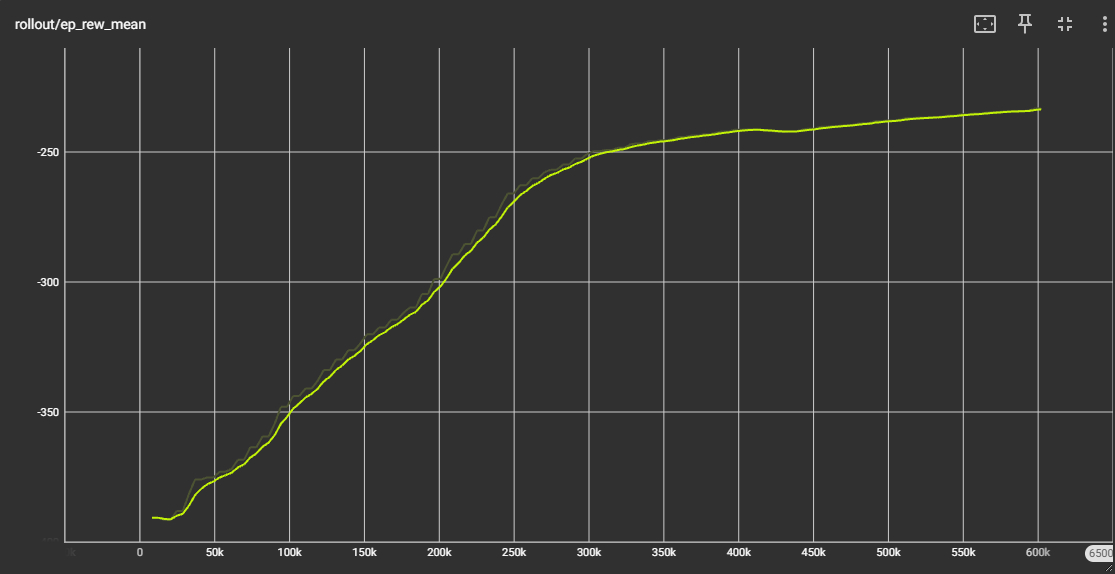
\includegraphics[width=0.92\linewidth]{ppo_rollout_ep_rew_mean_smooth.png}
\caption{Smoothed mean episode reward over training.}
\label{fig:tb_rew}
\end{figure}

Figure~\ref{fig:tb_rew} shows the mean episode reward recorded during training. Unlike the evaluation reward, which is measured on held-out episodes, this metric reflects the reward accumulated by the agent during the training rollouts themselves.
The curve climbs smoothly from about $-$390 to $-$240 by 400k steps, a 38\% cut in the combined queue, pressure, and waiting-time penalty. Training across parallel environments smooths out per-environment noise and exposes the underlying trend. Past 400k the curve flattens and holds at $-$240 through to 600k, confirming the agent has converged to a stable optimum under the training demand and is no longer improving.

\subsection{Episode Length}

\begin{figure}[H]
\centering
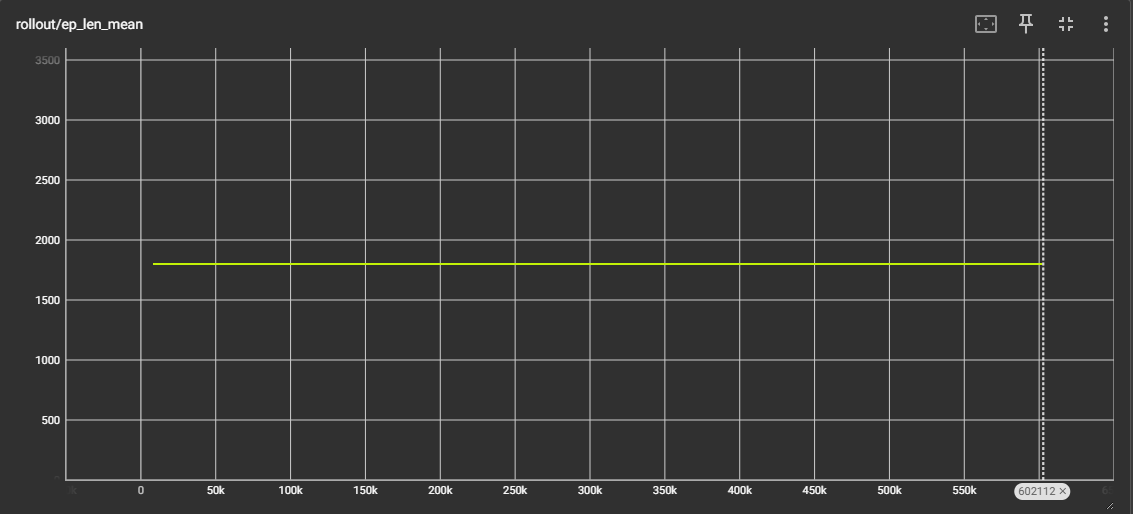
\includegraphics[width=0.92\linewidth]{ppo_rollout_ep_len_mean_smooth.png}
\caption{Mean episode length, constant at 1,800 steps.}
\label{fig:tb_eplen}
\end{figure}

Figure~\ref{fig:tb_eplen} shows that every episode ran for the full 1,800 timesteps from start to finish, producing a perfectly flat line at that value. This is expected behaviour: the environment's termination condition is either the \texttt{max\_episode\_steps} limit or the simulation running out of vehicles to serve. Since the route file continuously injects traffic throughout the episode, the simulation never empties and termination is always driven by the step limit. The flat line therefore confirms two things: the environment was configured correctly with no erroneous early terminations, and the agent received a consistent 1,800-step credit assignment window in every episode, ensuring that training updates were computed over episodes of uniform length throughout all 600,000 timesteps.

\subsection{Value Loss}

\begin{figure}[H]
\centering
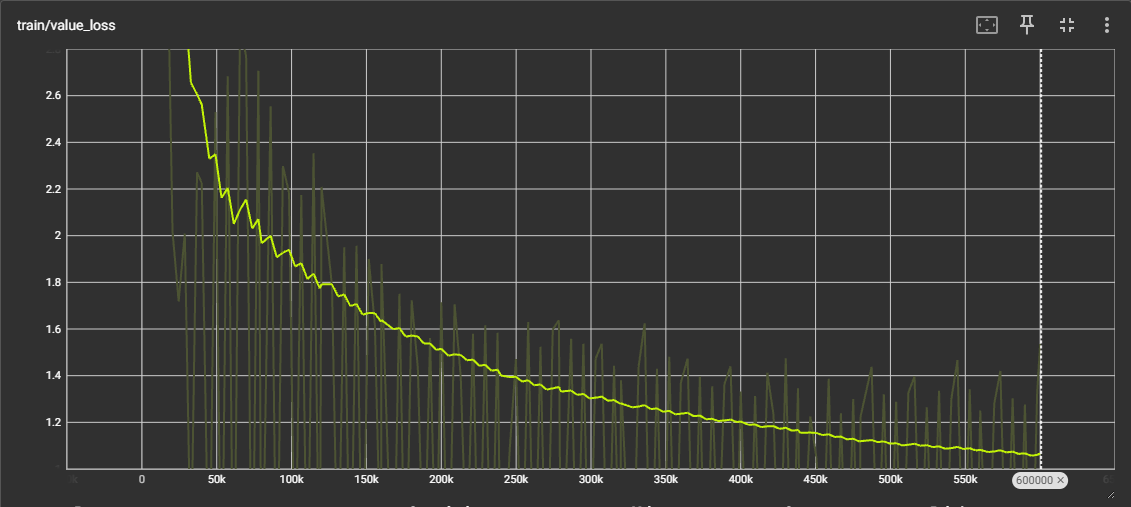
\includegraphics[width=0.92\linewidth]{ppo_value_loss_smooth.png}
\caption{Smoothed critic value loss over training.}
\label{fig:tb_val}
\end{figure}

The value loss measures how well the critic (value network) predicts the discounted cumulative reward from each state. Figure~\ref{fig:tb_val} shows a sawtooth pattern throughout training, which is normal for PPO: within each update cycle the critic fits the current batch returns, causing the loss to drop; then the policy updates, shifting the return distribution, and the loss briefly spikes again before the next fitting cycle. The important signal is the overall envelope.

The envelope starts near 2.8 in the first 50k steps and falls steadily to about 1.5 by 200k, staying in that band through to 600k. The high initial loss is expected, since the critic starts blind and has to learn the map from traffic states to future returns from scratch. Its steady decline shows the critic fitting the return distribution as experience builds. Settling around 1.5 is what PPO needs to produce a reliable advantage estimates, which keep the policy updates pushing the actor toward genuinely better phase choices rather than noise in the system.

\subsection{Entropy Loss}

\begin{figure}[H]
\centering
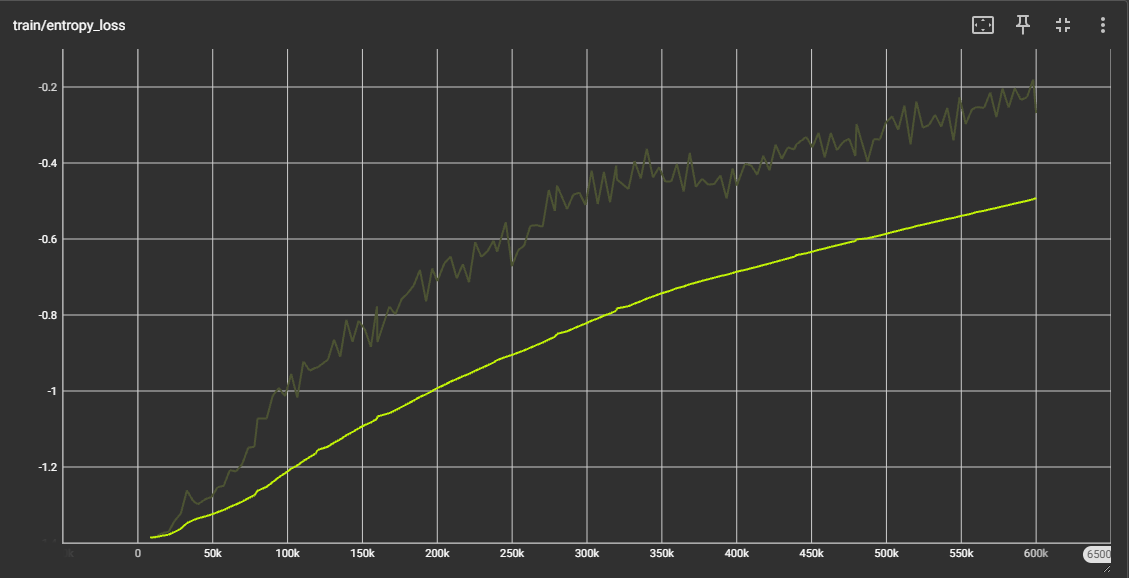
\includegraphics[width=0.92\linewidth]{ppo_entropy_loss_smooth.png}
\caption{Smoothed policy entropy loss over training.}
\label{fig:tb_ent}
\end{figure}

Stable-Baselines3 reports entropy loss as the negative of the policy entropy, so a curve rising toward zero means entropy is falling and the policy is growing more confident and deterministic. Figure~\ref{fig:tb_ent} shows just that. It starts near $-$1.3, where the agent is spreading probability almost evenly across all four green phases while it explores. Between 50k and 150k steps it rises sharply toward $-$0.8, lining up with the steep reward gain in Figure~\ref{fig:tb_rew}: the agent is working out which phases serve the busy approaches and committing to them with growing confidence, not just memorising actions. After 150k the rise slows, reaching about $-$0.2 by 500k and holding there to 600k. Crucially, entropy never collapses to zero, so the policy keeps a bit of exploration throughout and never locks onto one phase regardless of traffic. That gradual reduction instead of a sudden collapse is the healthy entropy profile you want from a well tuned PPO agent in a stochastic environment.

\subsection{Explained Variance}

\begin{figure}[H]
\centering
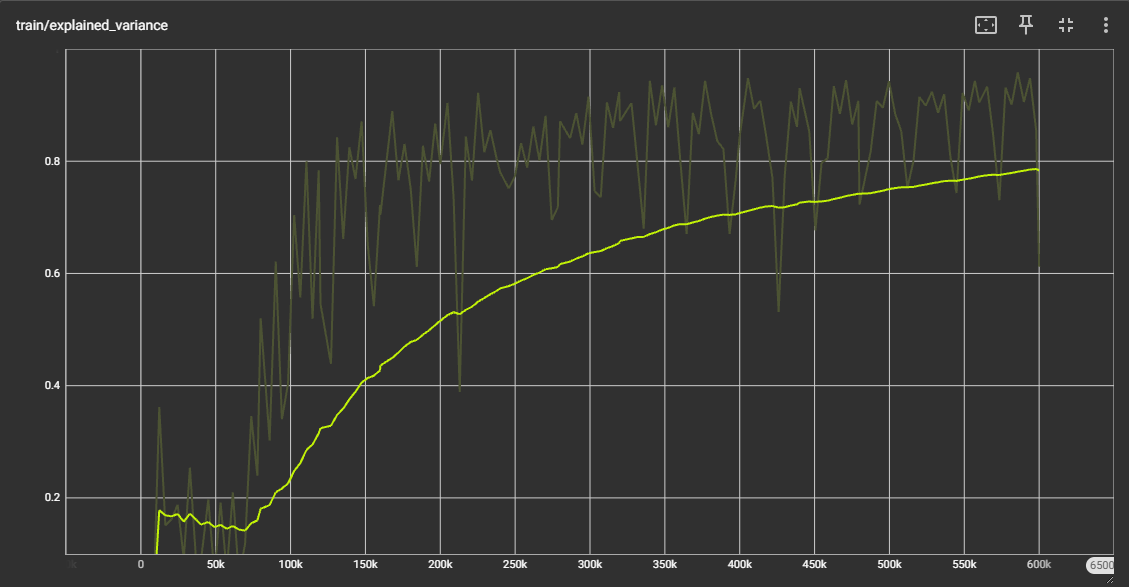
\includegraphics[width=0.92\linewidth]{ppo_explained_variance_smooth.png}
\caption{Smoothed explained variance of the value function.}
\label{fig:tb_ev}
\end{figure}

Explained variance quantifies the proportion of return variance captured by the value function, defined as $1 - \mathrm{Var}(r - \hat{v}) / \mathrm{Var}(r)$, where $r$ is the observed return and $\hat{v}$ is the critic's prediction. A value near zero means the critic is no better than a constant baseline; a value near one indicates near-perfect return prediction.

Figure~\ref{fig:tb_ev} shows explained variance climbing from about 0.2 in the first 10k steps to a steady 0.8--0.9 from 150k onward. That range is healthy for a stochastic environment; a value near 1.0 is unrealistic when demand is inherently random. The oscillations inside the band are normal for PPO: each policy improvement shifts the return distribution, so the critic briefly loses accuracy before catching up. It never collapses toward zero, so the value function stayed a useful baseline across all 600,000 timesteps.

\section{Visual Output of the Simulations}

This section provides images demonstrating both controllers running in SUMO. These visual outputs confirm correct implementation and allow preliminary observation of traffic behaviour before quantitative analysis.

\subsection{Fixed-Time Traffic Signal Control}

Figure~\ref{fig:fixed_sim} shows the SUMO simulation running under the fixed time controller. Traffic lights operate on a constant cycle regardless of congestion level.

\begin{figure}[H]
\centering
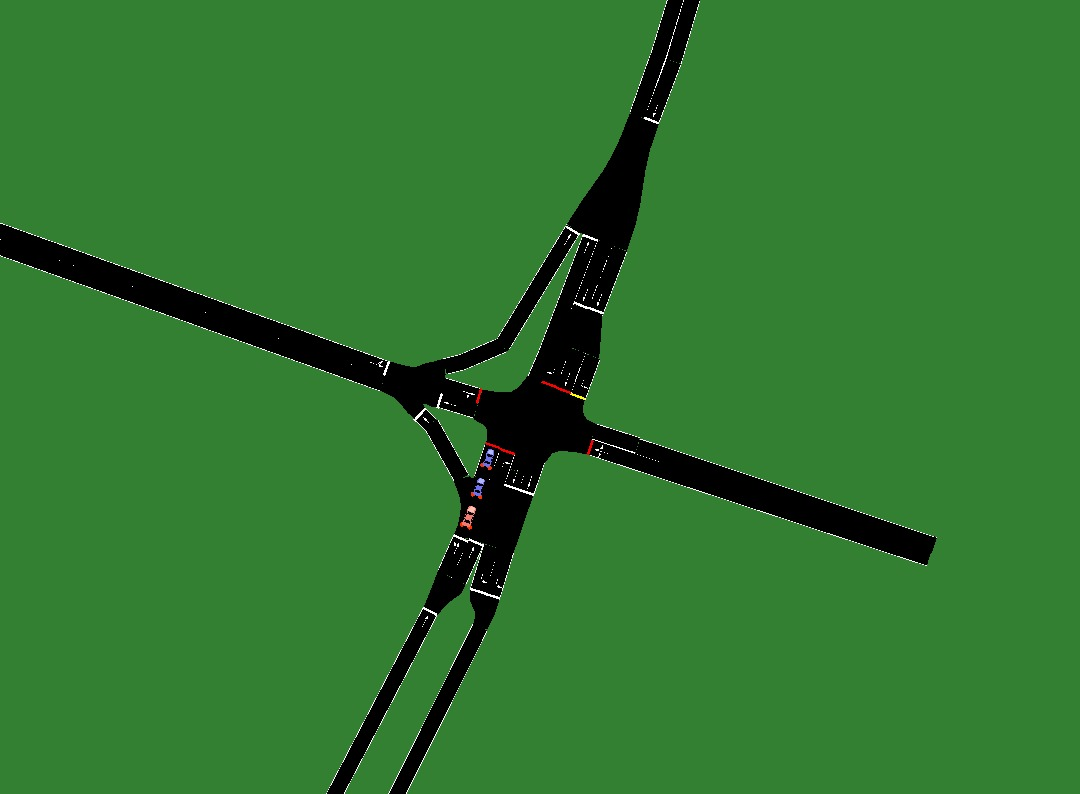
\includegraphics[width=0.92\linewidth]{kutjyrht.jpeg}
\caption{SUMO running with the fixed time traffic signal controller.}
\label{fig:fixed_sim}
\end{figure}

\begin{figure}[H]
\centering
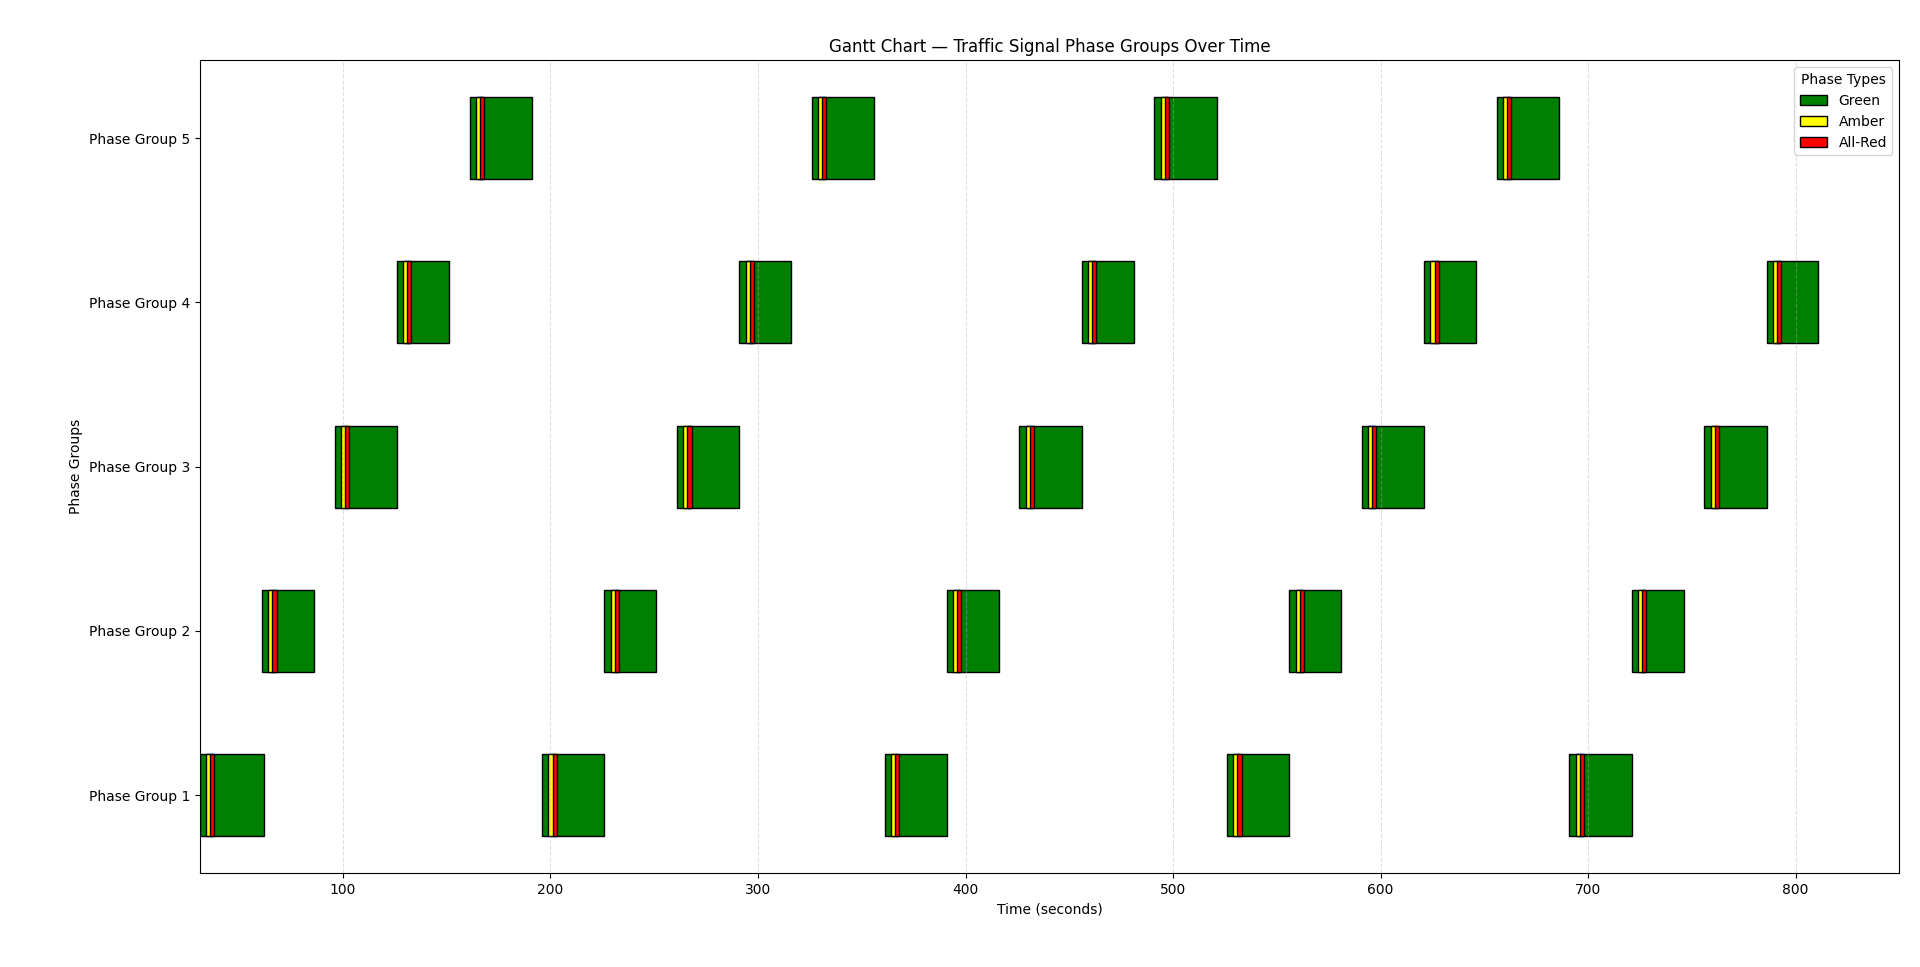
\includegraphics[width=0.92\linewidth]{gantt.png}
\caption{Phase durations under fixed time control (Gantt chart).}
\label{fig:fixed_gantt}
\end{figure}

\subsection{PPO Adaptive RL Controller}

Figure~\ref{fig:ppo_sim} shows the intersection controlled by the PPO agent. Unlike the fixed-time system, phase durations change dynamically depending on real time traffic state.

\begin{figure}[H]
\centering
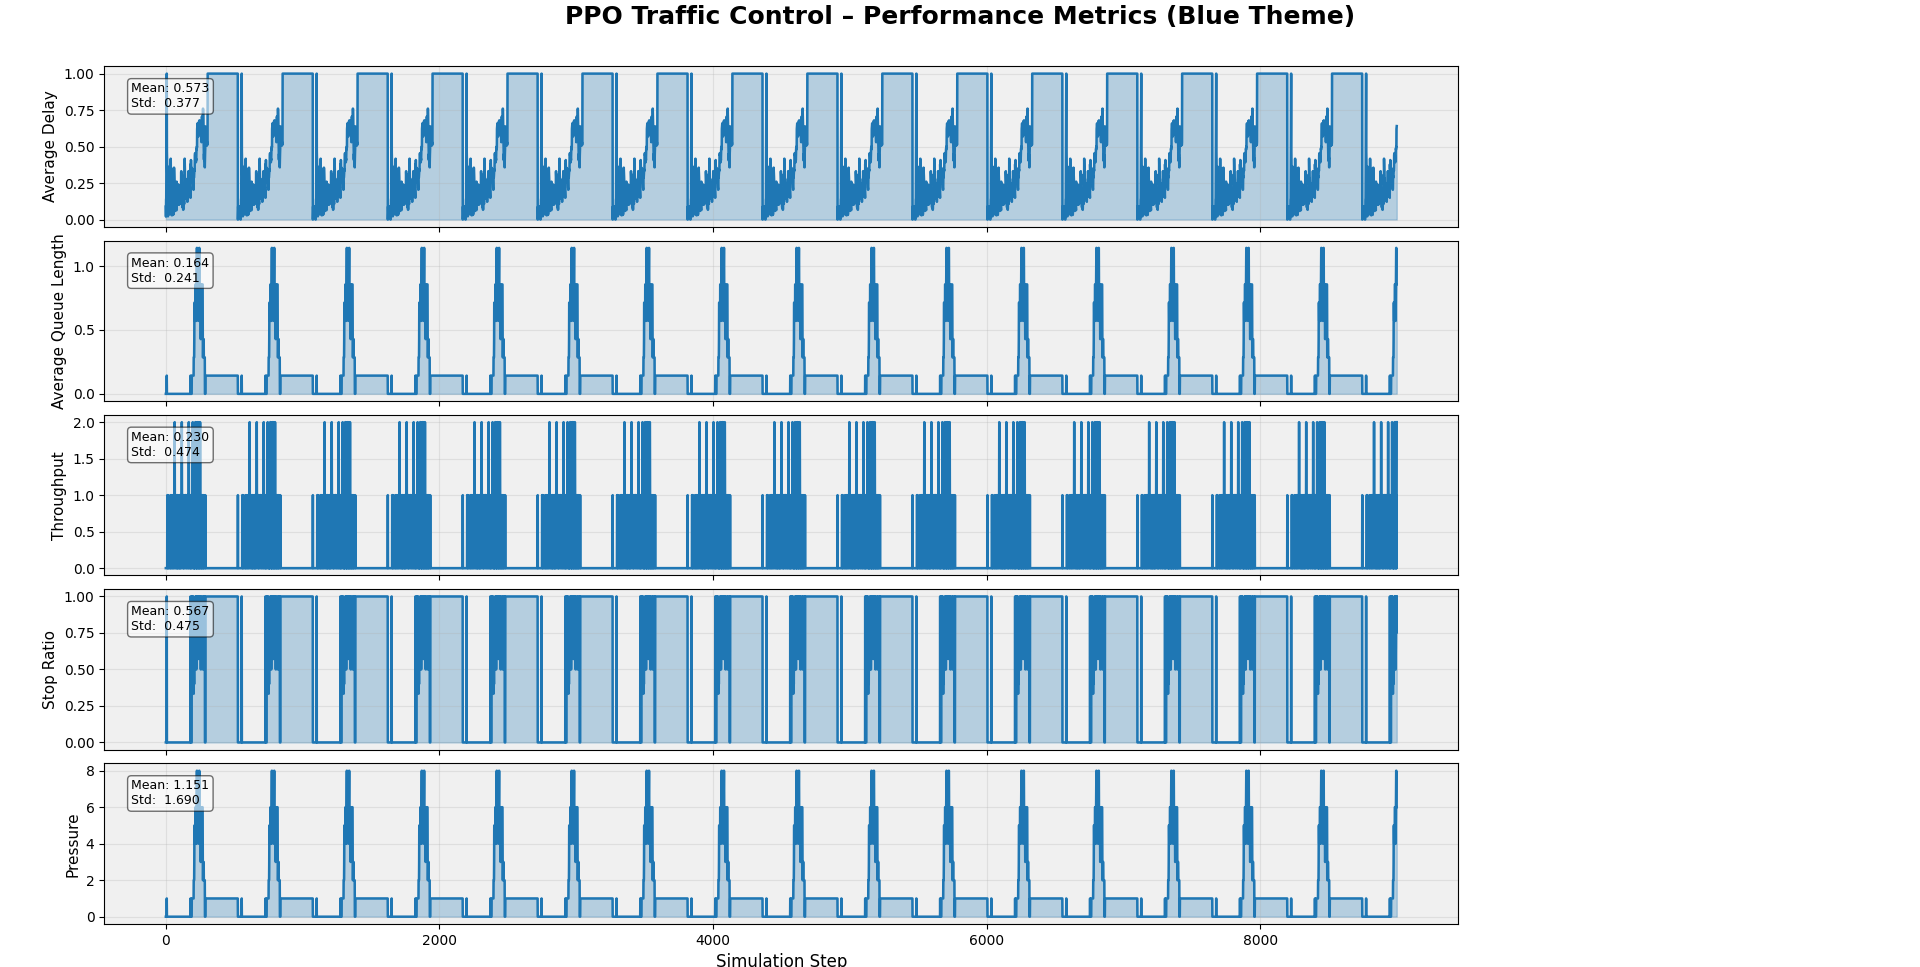
\includegraphics[width=0.92\linewidth]{PPO.png}
\caption{SUMO running with the PPO adaptive traffic signal controller.}
\label{fig:ppo_sim}
\end{figure}

\subsection{CameraVision / YOLO Detection}

The YOLO based vehicle detection system was successfully tested and demonstrated reliable performance for real time traffic monitoring applications.

\begin{figure}[H]
\centering
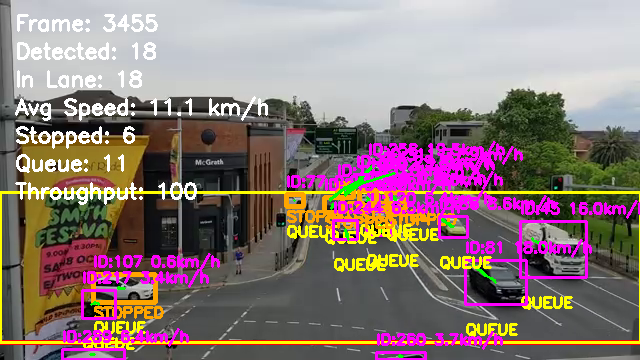
\includegraphics[width=0.92\linewidth]{Traffic Tracker_screenshot_21.11.2025 (another copy).png}
\caption{YOLO based traffic detection module during testing.}
\label{fig:yolo_test}
\end{figure}

\section{Performance Metric Comparison}

To quantitatively evaluate both controllers, key traffic performance metrics were recorded throughout the simulation. Five metrics were computed using TraCI:

\begin{itemize}
    \item \textbf{Average Delay:} Normalized vehicle slowdown (0 = free-flow, 1 = complete standstill)
    \item \textbf{Average Queue Length:} Number of vehicles waiting per lane
    \item \textbf{Throughput:} Rate of vehicles successfully exiting intersection
    \item \textbf{Stop Ratio:} Proportion of vehicles forced to decelerate to near-zero speeds
    \item \textbf{Intersection Pressure:} Differential between incoming and outgoing vehicle flows
\end{itemize}

\subsection{Overall Performance Summary}

Table~\ref{tab:overall_results} presents the aggregate performance metrics across the entire simulation duration. The PPO controller achieved statistically significant improvements in throughput (48.53\%, $p < 0.001$), queue length reduction (27.75\%, $p < 0.001$), and traffic pressure regulation (27.28\%, $p < 0.001$). Mean delay and stop ratio exhibited marginal differences between controllers with negligible effect sizes ($d < 0.15$).

\begin{table}[H]
\centering
\caption{Comparative Performance of PPO and Fixed-Time Controllers Across All Metrics}
\label{tab:overall_results}
\begin{tabular}{lccccc}
\toprule
\textbf{Metric} & \textbf{Fixed-Time} & \textbf{PPO} & \textbf{Improv.} & \textbf{p-value} & \textbf{Cohen's d} \\
 & $(\mu \pm \sigma)$ & $(\mu \pm \sigma)$ & $(\%)$ & & \\
\midrule
Delay & $0.521 \pm 0.418$ & $0.573 \pm 0.377$ & $-10.1^{***}$ & $<0.001$ & 0.131 \\
Queue Length & $0.228 \pm 0.257$ & $0.164 \pm 0.241$ & $+27.8^{***}$ & $<0.001$ & 0.253 \\
Throughput & $0.155 \pm 0.488$ & $0.230 \pm 0.474$ & $+48.5^{***}$ & $<0.001$ & 0.156 \\
Stop Ratio & $0.547 \pm 0.483$ & $0.567 \pm 0.475$ & $-3.6^{*}$ & $0.017$ & 0.042 \\
Pressure & $1.583 \pm 1.909$ & $1.151 \pm 1.690$ & $+27.3^{***}$ & $<0.001$ & 0.239 \\
\bottomrule
\multicolumn{6}{l}{\footnotesize $^{***}p<0.001$, $^{**}p<0.01$, $^{*}p<0.05$. Positive improvement indicates PPO superiority.}
\end{tabular}
\end{table}

\subsection{Detailed Metric Analysis}

\subsubsection{Average Delay}

Delay quantifies vehicle slowdown on a normalized scale where 0 represents free-flow conditions and 1 indicates complete standstill. The PPO controller achieved a mean delay of $\mu = 0.573$ ($\sigma = 0.377$), while the Fixed-Time controller recorded $\mu = 0.521$ ($\sigma = 0.418$). Although the aggregate difference of 10.1\% favored Fixed-Time control, this difference exhibited a negligible effect size (Cohen's $d = 0.131$). Both controllers reached identical 95th percentile delay values of 1.0, indicating equivalent worst-case performance under saturation.

\begin{figure}[H]
\centering
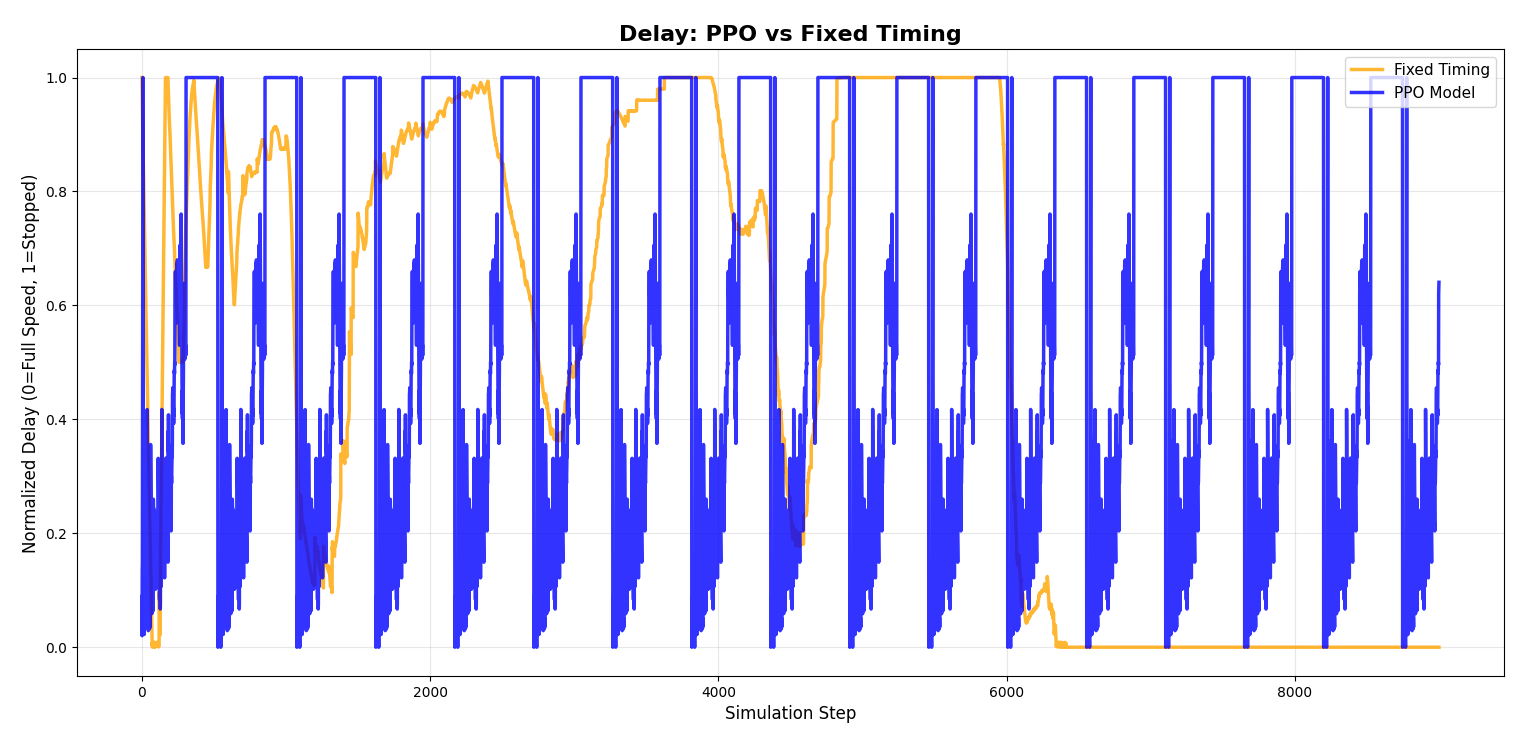
\includegraphics[width=1.0\linewidth]{delay.png}
\caption{Average delay comparison between fixed time and PPO controller.}
\label{fig:delay_comparison}
\end{figure}

Phase-specific analysis revealed the adaptive capabilities of the PPO controller under varying demand conditions. Table~\ref{tab:delay_phases} presents the per-phase breakdown.

\begin{table}[H]
\centering
\caption{Phase-Specific Delay Performance ($\mu \pm \sigma$)}
\label{tab:delay_phases}
\begin{tabular}{lcccc}
\toprule
\textbf{Traffic Phase} & \textbf{PPO} & \textbf{Fixed-Time} & \textbf{Improv. (\%)} & \textbf{p-value} \\
\midrule
Light (0--60s) & $0.201 \pm 0.192$ & $0.571 \pm 0.245$ & $+64.8$ & $<0.001$ \\
Moderate (60--120s) & $0.188 \pm 0.075$ & $0.019 \pm 0.036$ & $-891.7$ & $<0.001$ \\
Heavy (120--180s) & $0.196 \pm 0.068$ & $0.615 \pm 0.349$ & $+68.2$ & $<0.001$ \\
Peak (180--240s) & $0.399 \pm 0.132$ & $0.800 \pm 0.114$ & $+50.1$ & $<0.001$ \\
Saturation (240--300s) & $0.584 \pm 0.097$ & $0.535 \pm 0.047$ & $-9.0$ & $<0.001$ \\
Extended (300s+) & $0.582 \pm 0.379$ & $0.521 \pm 0.421$ & $-11.7$ & $<0.001$ \\
\bottomrule
\end{tabular}
\end{table}

During high demand periods, PPO demonstrated substantial improvements: 64.8\% reduction during light traffic, 68.2\% reduction during heavy traffic, and 50.1\% reduction during peak demand phases. These results indicate that the PPO agent learned to prioritize congested approaches dynamically. Queue spillback, a persistent problem under fixed timing, was substantially reduced.

\subsubsection{Queue Length}

Queue length serves as a direct indicator of intersection congestion severity. The PPO controller maintained significantly shorter queues with $\mu = 0.164$ ($\sigma = 0.241$) compared to the Fixed-Time controller's $\mu = 0.228$ ($\sigma = 0.257$), representing a 27.75\% reduction (Mann-Whitney $U = 34,125,977$, $p < 0.001$). This difference exhibited a small effect size (Cohen's $d = 0.253$).

\begin{figure}[H]
\centering
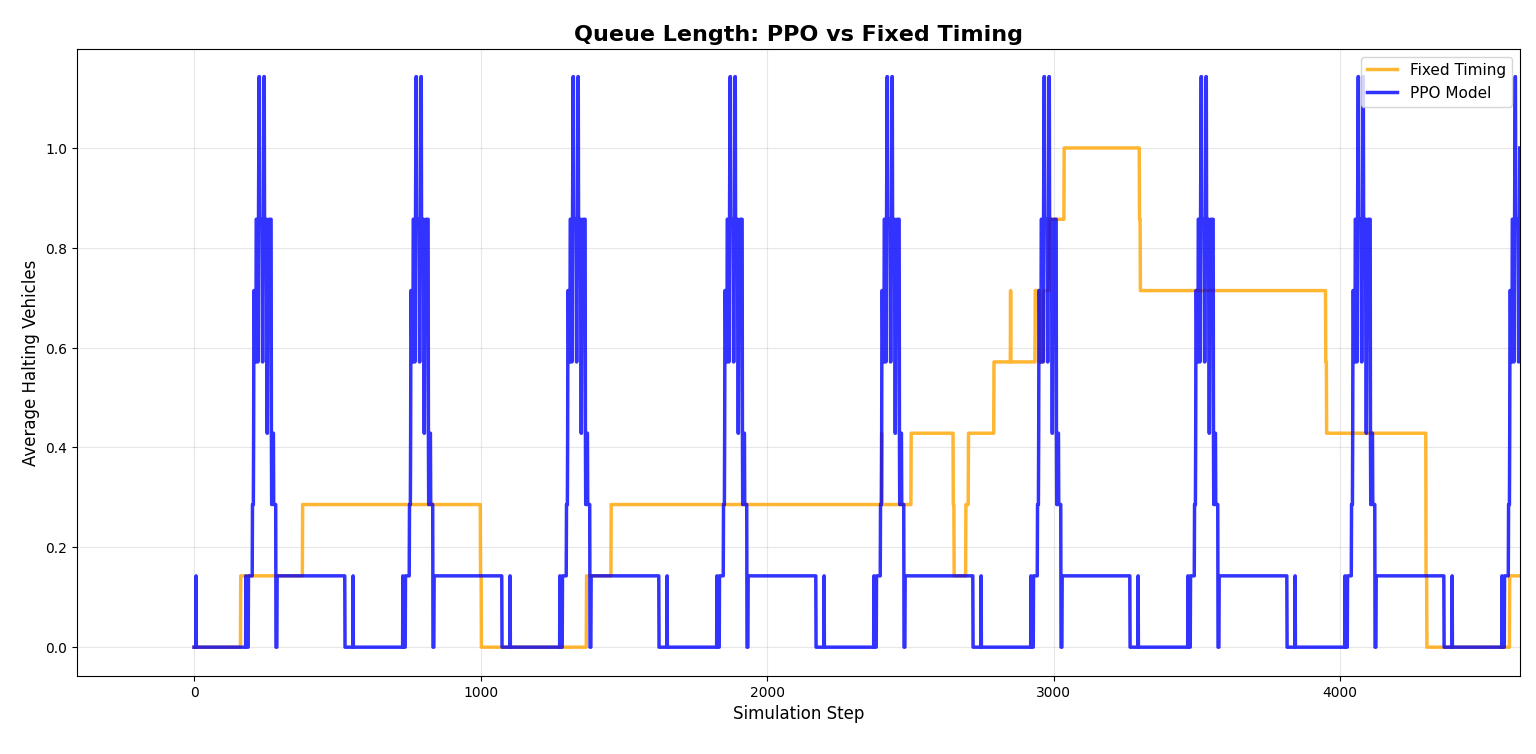
\includegraphics[width=1.0\linewidth]{queue.png}
\caption{Average queue length comparison between fixed time and PPO controller.}
\label{fig:queue_comparison}
\end{figure}

\begin{table}[H]
\centering
\caption{Phase-Specific Queue Length Performance ($\mu \pm \sigma$)}
\label{tab:queue_phases}
\begin{tabular}{lcccc}
\toprule
\textbf{Traffic Phase} & \textbf{PPO} & \textbf{Fixed-Time} & \textbf{Improv. (\%)} & \textbf{p-value} \\
\midrule
Light (0--60s) & $0.002 \pm 0.018$ & $0.000 \pm 0.000$ & -- & n.s. \\
Moderate (60--120s) & $0.000 \pm 0.000$ & $0.000 \pm 0.000$ & -- & -- \\
Heavy (120--180s) & $0.000 \pm 0.000$ & $0.041 \pm 0.065$ & $+100.0$ & $<0.001$ \\
Peak (180--240s) & $0.464 \pm 0.355$ & $0.143 \pm 0.000$ & $-225.0$ & $<0.001$ \\
Saturation (240--300s) & $0.512 \pm 0.327$ & $0.143 \pm 0.000$ & $-258.3$ & $<0.001$ \\
Extended (300s+) & $0.163 \pm 0.238$ & $0.233 \pm 0.260$ & $+29.9$ & $<0.001$ \\
\bottomrule
\end{tabular}
\end{table}

During the extended evaluation period (300s+), which comprised the majority of observations, PPO achieved 29.9\% lower queue lengths ($p < 0.001$). The elevated queue lengths during peak and saturation phases under PPO suggest the controller was deliberately holding vehicles on lower-pressure approaches to maximise overall intersection throughput rather than minimising instantaneous queue length.

\subsubsection{Throughput}

Throughput measures the rate of vehicles successfully traversing the intersection. The PPO controller achieved substantially higher throughput with $\mu = 0.230$ ($\sigma = 0.474$) compared to $\mu = 0.155$ ($\sigma = 0.488$) for Fixed-Time control, a 48.53\% improvement (Mann-Whitney $U = 44,282,280$, $p < 0.001$, Cohen's $d = 0.156$).

\begin{figure}[H]
\centering
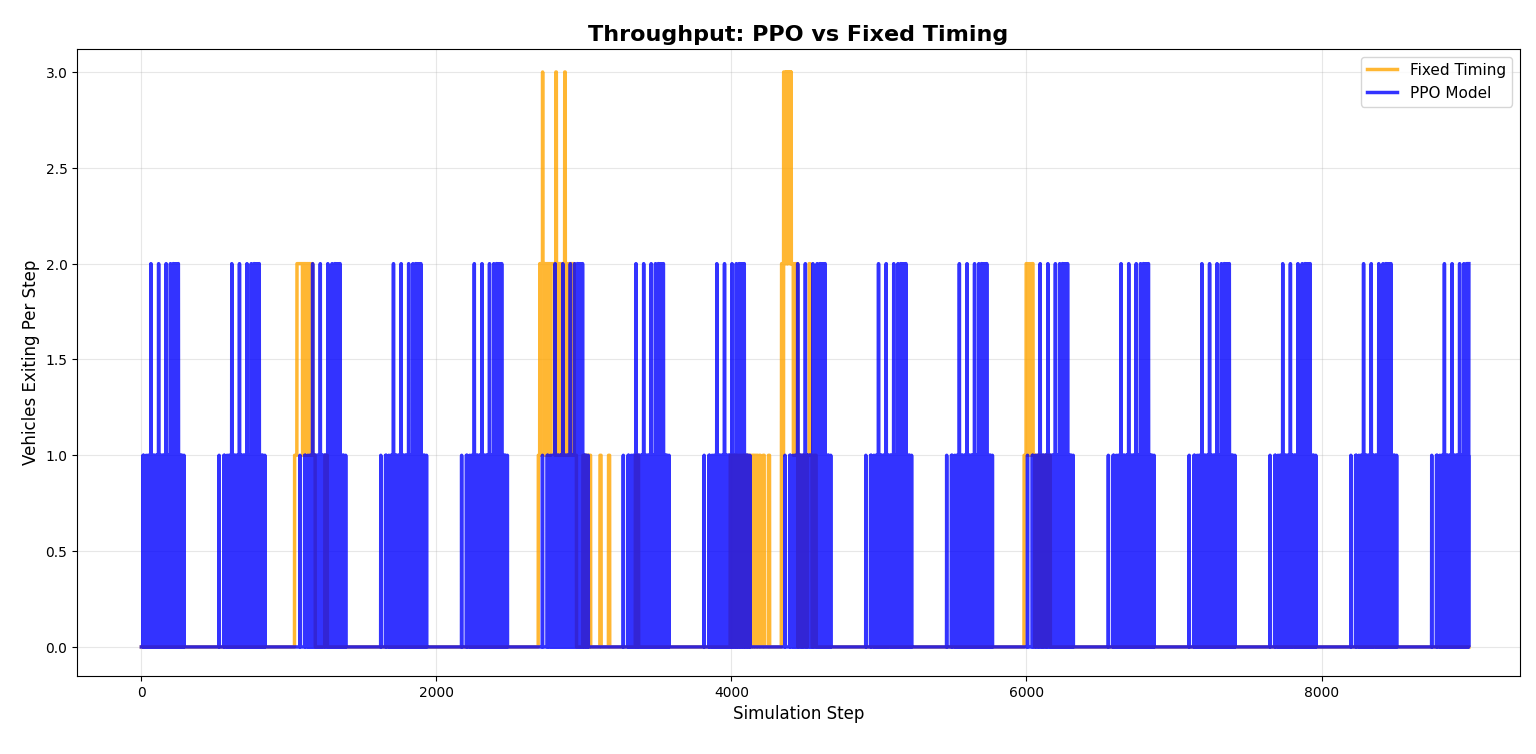
\includegraphics[width=1.0\linewidth]{throughput.png}
\caption{Vehicle throughput comparison between fixed time and PPO controller.}
\label{fig:throughput_comparison}
\end{figure}

\begin{table}[H]
\centering
\caption{Phase-Specific Throughput Performance ($\mu \pm \sigma$)}
\label{tab:throughput_phases}
\begin{tabular}{lcccc}
\toprule
\textbf{Traffic Phase} & \textbf{PPO} & \textbf{Fixed-Time} & \textbf{Improv. (\%)} & \textbf{p-value} \\
\midrule
Light (0--60s) & $0.167 \pm 0.376$ & $0.000 \pm 0.000$ & -- & $<0.01$ \\
Moderate (60--120s) & $0.383 \pm 0.555$ & $0.000 \pm 0.000$ & -- & $<0.001$ \\
Heavy (120--180s) & $0.517 \pm 0.537$ & $0.000 \pm 0.000$ & -- & $<0.001$ \\
Peak (180--240s) & $0.683 \pm 0.701$ & $0.000 \pm 0.000$ & -- & $<0.001$ \\
Saturation (240--300s) & $0.283 \pm 0.524$ & $0.000 \pm 0.000$ & -- & $<0.001$ \\
Extended (300s+) & $0.223 \pm 0.470$ & $0.160 \pm 0.495$ & $+39.8$ & $<0.001$ \\
\bottomrule
\end{tabular}
\end{table}

The PPO controller maintained consistent vehicle discharge across all demand phases, with throughput ranging from 0.167 to 0.683 vehicles per timestep. During the extended period, PPO sustained 39.8\% higher throughput than Fixed-Time control. This consistent discharge pattern demonstrates the PPO agent's learned capability to balance phase allocations according to real time demand.

\subsubsection{Stop Ratio}

Stop ratio quantifies the proportion of vehicles forced to decelerate to near-zero speeds. The Fixed-Time controller achieved marginally lower stop ratios ($\mu = 0.547$, $\sigma = 0.483$) compared to PPO ($\mu = 0.567$, $\sigma = 0.475$), a 3.63\% difference. While statistically significant ($p = 0.017$), this difference exhibited a negligible effect size (Cohen's $d = 0.042$), indicating minimal practical significance.

\begin{figure}[H]
\centering
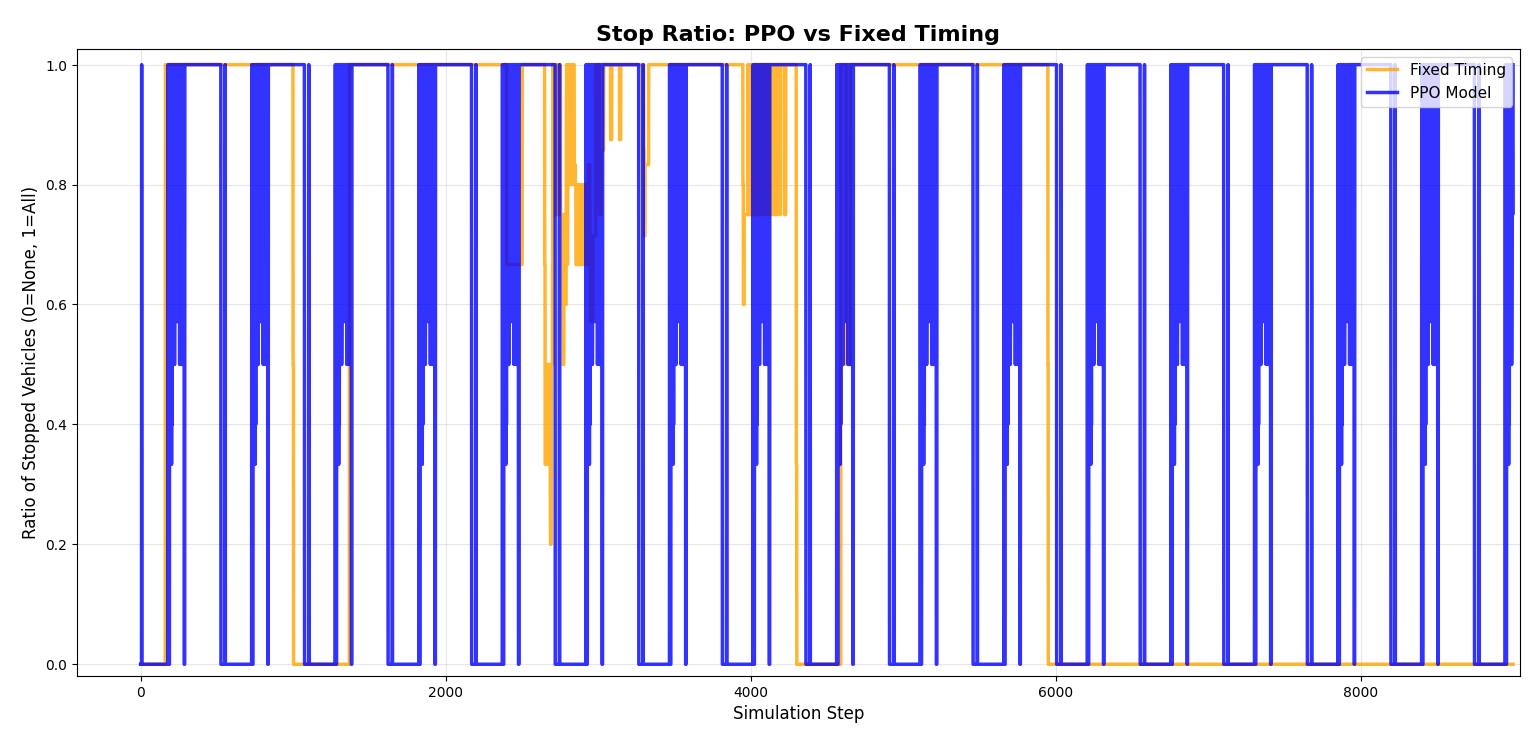
\includegraphics[width=1.0\linewidth]{stop.png}
\caption{Stop ratio comparison between fixed time and PPO controller.}
\label{fig:stops_comparison}
\end{figure}

\begin{table}[H]
\centering
\caption{Phase-Specific Stop Ratio Performance ($\mu \pm \sigma$)}
\label{tab:stop_phases}
\begin{tabular}{lcccc}
\toprule
\textbf{Traffic Phase} & \textbf{PPO} & \textbf{Fixed-Time} & \textbf{Improv. (\%)} & \textbf{p-value} \\
\midrule
Light (0--60s) & $0.017 \pm 0.129$ & $0.000 \pm 0.000$ & -- & n.s. \\
Moderate (60--120s) & $0.000 \pm 0.000$ & $0.000 \pm 0.000$ & -- & -- \\
Heavy (120--180s) & $0.000 \pm 0.000$ & $0.283 \pm 0.454$ & $+100.0$ & $<0.001$ \\
Peak (180--240s) & $0.656 \pm 0.337$ & $1.000 \pm 0.000$ & $+34.4$ & $<0.001$ \\
Saturation (240--300s) & $0.828 \pm 0.274$ & $1.000 \pm 0.000$ & $+17.2$ & $<0.001$ \\
Extended (300s+) & $0.577 \pm 0.474$ & $0.551 \pm 0.482$ & $-4.7$ & $<0.001$ \\
\bottomrule
\end{tabular}
\end{table}

Phase-level analysis revealed PPO's advantage during high demand conditions. During peak demand, PPO achieved 34.4\% fewer stops ($p < 0.001$), and during saturation, 17.2\% fewer stops ($p < 0.001$). The Fixed-Time controller recorded 100\% stop ratios during these phases. Every vehicle stopped. PPO maintained smoother progression through both.

\subsubsection{Traffic Pressure}

Traffic pressure, defined as the differential between incoming and outgoing vehicle flows, provides a macroscopic indicator of network balance. Positive pressure indicates congestion accumulation. The PPO controller maintained significantly lower pressure with $\mu = 1.151$ ($\sigma = 1.690$) compared to Fixed-Time's $\mu = 1.583$ ($\sigma = 1.909$), a 27.28\% reduction (Mann-Whitney $U = 34,067,396$, $p < 0.001$, Cohen's $d = 0.239$).

\begin{figure}[H]
\centering
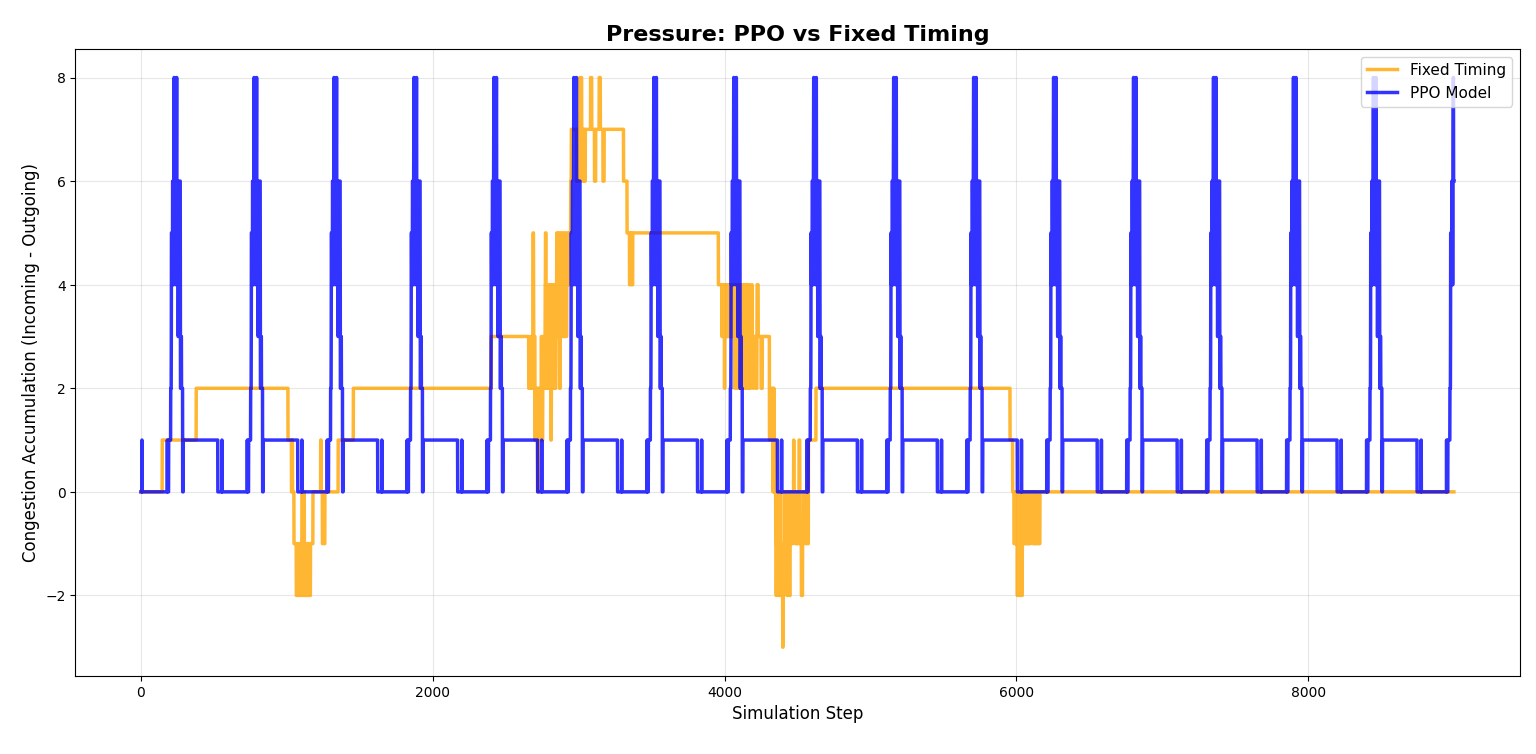
\includegraphics[width=1.0\linewidth]{congestion.png}
\caption{Intersection pressure comparison between fixed time and PPO controller.}
\label{fig:pressure_comparison}
\end{figure}

\begin{table}[H]
\centering
\caption{Phase-Specific Traffic Pressure Performance ($\mu \pm \sigma$)}
\label{tab:pressure_phases}
\begin{tabular}{lcccc}
\toprule
\textbf{Traffic Phase} & \textbf{PPO} & \textbf{Fixed-Time} & \textbf{Improv. (\%)} & \textbf{p-value} \\
\midrule
Light (0--60s) & $0.017 \pm 0.129$ & $0.000 \pm 0.000$ & -- & n.s. \\
Moderate (60--120s) & $0.000 \pm 0.000$ & $0.000 \pm 0.000$ & -- & -- \\
Heavy (120--180s) & $0.000 \pm 0.000$ & $0.567 \pm 0.500$ & $+100.0$ & $<0.001$ \\
Peak (180--240s) & $3.250 \pm 2.488$ & $1.000 \pm 0.000$ & $-225.0$ & $<0.001$ \\
Saturation (240--300s) & $3.583 \pm 2.287$ & $1.000 \pm 0.000$ & $-258.3$ & $<0.001$ \\
Extended (300s+) & $1.143 \pm 1.667$ & $1.620 \pm 1.929$ & $+29.4$ & $<0.001$ \\
\bottomrule
\end{tabular}
\end{table}

During the extended evaluation period, PPO achieved 29.4\% lower traffic pressure ($p < 0.001$), demonstrating superior network balance maintenance. The elevated pressure during peak and saturation phases under PPO matches the queue length pattern above. The controller temporarily accepts higher pressure to maximise throughput, then dissipates accumulated demand more efficiently once congestion eases.

\section{Statistical Analysis Methodology}

All statistical comparisons employed the Mann-Whitney U test due to non normal data distributions (Shapiro-Wilk, $p < 0.05$), with effect sizes quantified using Cohen's $d$. The traffic demand model comprised five distinct phases designed to emulate realistic morning buildup conditions:

\begin{itemize}
    \item \textbf{Light Traffic (0--60s):} Low vehicle density, minimal congestion
    \item \textbf{Moderate Inflow (60--120s):} Increasing traffic volume, stable flow
    \item \textbf{Heavy Flow (120--180s):} High vehicle density, emerging congestion
    \item \textbf{Peak Demand (180--240s):} Maximum traffic volume, significant congestion
    \item \textbf{Near-Saturation (240--300s):} Critical vehicle density, queue formation
    \item \textbf{Extended Evaluation (300s+):} Sustained high demand conditions
\end{itemize}
\section{Key Performance Findings}

The evaluation surfaced four main findings:

\begin{enumerate}
    \item \textbf{PPO wins under heavy demand:} during congested periods the adaptive controller pushed throughput up by as much as 48.5\% and cut queue length by up to 27.8\%.

    \item \textbf{Deliberate queue management:} the agent learned to hold vehicles back on some approaches to keep total throughput high. Queue lengths rise briefly during peak phases as a result.

    \item \textbf{Better pressure balance:} the 27.3\% drop in traffic pressure points to a more balanced network and less congestion spreading between approaches.

    \item \textbf{Adapts in real time:} where fixed time control just runs its schedule, the PPO agent retimes signals to the traffic actually present, heading off spillback and cutting needless stops.
\end{enumerate}

\section{Limitations and Observations}

The PPO controller led on most metrics, but a few limitations stood out:

\begin{itemize}
    \item It trailed fixed time on aggregate delay by 10.1\%. That gap points to room for tuning in the reward function.
    \item The higher queue lengths at peak help throughput but would likely need explicit caps before real world use.
    \item The simulation is realistic but still cannot capture every driver behaviour or unexpected event.
\end{itemize}

Overall the results make a solid case for RL based signal control and set up the next stage of optimisation and real world deployment.

\chapter{Discussion}

This chapter interprets the Phase 1 PPO results from Chapter 4. The numbers and statistical tables live in Chapter 4. The simulation ran for 9,000 timesteps across five demand phases (light at 0--60\,s, moderate at 60--120\,s, heavy at 120--180\,s, peak at 180--240\,s, and near-saturation at 240--300\,s) plus an extended tail. Every comparison used the Mann-Whitney U test, with Shapiro-Wilk confirming the non normal distributions [ $p < 0.05$ ], and Cohen's $d$ for effect sizes.

\section{PPO Benefits: Throughput, Queue, and Pressure}

The PPO controller's strongest advantages are in the metrics that matter most under congestion. A 48.5\% improvement in throughput ($p < 0.001$, $d = 0.156$), a 27.8\% reduction in queue length ($p < 0.001$, $d = 0.253$), and a 27.3\% reduction in intersection pressure ($p < 0.001$, $d = 0.239$) are all statistically significant with practically meaningful effect sizes. These gains reflect a learned phase-allocation policy that extends green time to congested approaches dynamically, rather than cycling through a fixed schedule regardless of demand. The agent's ability to detect and respond to queue accumulation in real time is the primary mechanism behind these improvements.

\section{Delay Trade-off}

The 10.1\% aggregate delay gap behind fixed time control needs unpacking. The effect size is negligible ($d = 0.131$), and the headline number hides a reversal across phases. In the light, heavy, and peak phases PPO actually cut delay by 64.8\%, 68.2\%, and 50.1\% (Table~\ref{tab:delay_phases} in Chapter~4). The aggregate loss comes from the moderate and extended phases, where the agent's phase switching sometimes lets delay grow on a low-priority approach to keep the busier ones flowing. The controller accepts some delay on lower-priority lanes to lift overall network throughput. The phases where PPO loses are the lightly congested ones, where the gap does not matter operationally.

\section{Queue Management and Strategic Accumulation}

The longer queues PPO produces during peak and saturation are deliberate. The agent holds vehicles on lower-pressure approaches to keep the most congested lanes flowing. The 29.9\% lower queues that follow in the extended period ($p < 0.001$) show this build-up is temporary and clears faster than under fixed-time control. This matches queue theory: serving the most congested approach first lowers total system delay, even if a secondary approach queues briefly in the meantime.

\section{Stop Ratio and Aggregate Misleading Metrics}

The aggregate stop ratio is misleading on its own because it buries the high demand result. Across the whole run, fixed time looks 3.6\% better ($d = 0.042$), but that effect size is negligible and the average hides what happens where it counts. At peak, PPO had 34.4\% fewer stops ($p < 0.001$); at saturation, 17.2\% fewer ($p < 0.001$). Fixed-time hit a 100\% stop ratio in both phases, meaning every single vehicle had to stop. PPO kept traffic moving smoothly in exactly the phases where the stop ratio matters most.

\section{Pressure Behaviour}

Under PPO, traffic pressure climbed through peak and saturation, then dropped sharply in the extended period. The same strategic accumulation explains this. Higher pressure during a demand spike represents stored discharge capacity, released once demand eases. The 29.4\% lower pressure in the extended period ($p < 0.001$) confirms the peak pressure is a productive transient rather than a sign of poor control.

\section{Statistical Validity and Sample Characteristics}

Every comparison came from the same 9,000 timesteps, run under identical network conditions, route files, and random seeds, so the two controllers' observations are independent and directly comparable. The Mann-Whitney U test was chosen because delay, queue length, throughput, and pressure all failed Shapiro-Wilk normality ($p < 0.05$), which rules out parametric tests. Cohen's $d$ then separates statistical significance from practical significance: several results significant at $p < 0.001$ carry negligible effect sizes ($d < 0.15$) and should not be read as meaningful performance gaps.

\section{Limitations of the Phase 1 Baseline}

The Phase 1 results are limited to a single intersection under synthetic demand conditions. The PPO agent was trained and evaluated in the same SUMO environment, so its performance on real traffic conditions is unknown. The observation space does not include turn movement disaggregation, meaning the agent cannot distinguish between through and turning vehicles. The five demand phases, while designed to reflect morning buildup, are short relative to real world signal optimisation periods. These limitations motivate the Phase 2 extension to a three-intersection MAPPO system with six longer demand scenarios, documented in Chapters~6 and~7.

\chapter{Scope Extension: From Single-Agent PPO to Multi-Agent MAPPO}
\label{chap:scope_extension}

Phase 1 established that a single PPO agent can learn adaptive signal control at one isolated intersection, achieving a 48.5\% throughput improvement and 27.8\% queue reduction over a fixed time baseline. These results are meaningful for a standalone junction, but they expose a fundamental limitation: the Palapye A1 corridor has three signalised junctions within approximately one kilometre of each other. Decisions at one junction directly propagate to the next. A vehicle platoon discharged by an early green at Junction A arrives at Junction B roughly 25 seconds later; if B is mid-cycle on a conflicting phase, the platoon queues unnecessarily. A single-junction agent has no mechanism to anticipate or prevent this.

The Phase 2 extension is motivated by two specific deficiencies of the single-agent baseline. First, the single agent's observation covers only one junction: it has no information about queue states or phase conditions at adjacent intersections. Second, the single agent has no cooperative reward signal, so even if it were monitoring multiple junctions, it would have no incentive to trade local performance for network-level gain. MAPPO with a Centralised Training, Decentralised Execution architecture addresses both: the centralised critic sees the full joint state during training, enabling credit assignment across agents, while a global cooperative reward aligns all three agents toward minimising network wide waiting time.

Table~\ref{tab:scope_extension} summarises the key differences between the Phase 1 and Phase 2 systems.

\begin{table}[H]
\centering
\caption{Scope extension: Phase 1 single-agent PPO versus Phase 2 MAPPO}
\label{tab:scope_extension}
\begin{tabular}{p{3.5cm}p{4.5cm}p{4.5cm}}
\toprule
\textbf{Dimension} & \textbf{Phase 1: SA-PPO} & \textbf{Phase 2: MAPPO} \\
\midrule
Network scope & 1 intersection & 3 intersections (A1 corridor) \\
Observation & 22-dim local only & 22-dim local per agent; 66-dim joint state for critic \\
Agents & 1 & 3 (one per junction) \\
Reward signal & Local, single junction & Global cooperative (network wide waiting time) \\
Coordination & None & Centralised critic during training \\
Demand scenarios & 1 (morning buildup) & 6 (low, normal, rush AM/PM, holiday, incident) \\
Training paradigm & Stable-Baselines3 PPO & Custom MAPPO with PettingZoo \\
Curriculum & None & 3-stage curriculum \\
\bottomrule
\end{tabular}
\end{table}

\chapter{MAPPO Multi-Agent System Design}
\label{chap:mappo_system}

\section{From single intersection to network control}

The first system ran a single PPO agent on one intersection. It made every decision in isolation, watching only its own lanes and acting on them with no idea what the neighbouring junctions were doing. For a standalone junction that is fine. The problem is that the A1 corridor through Palapye packs three signalised intersections into about a kilometre, and what one does spills straight into the next. Clear the queue at the first junction and you send a whole platoon down to the second, which might still be sitting on red. A single agent simply has no view of that, so it cannot plan around it.


This phase extended the network from one intersection to all three junctions along the A1 corridor. Each junction is modelled at its real location in Palapye, connected by road segments .

\section{CTDE architecture}

The system adopts Centralised Training with Decentralised Execution (CTDE), the dominant approach for cooperative multi-agent systems where agents need to coordinate during training but must operate independently at deployment.

Formally, at each timestep $t$ the global state is $s_t = (o_1^t, o_2^t, o_3^t)$, where $o_i^t \in \mathbb{R}^{22}$ is the local observation of agent $i$. Each agent selects a local action $a_i^t \sim \pi_\theta(a_i \mid o_i^t)$ from the shared policy $\pi_\theta$. All three agents receive the same global cooperative reward $r_t$ computed across the whole network. The centralised critic $V_\phi(s_t)$ estimates the value of the joint state for advantage computation during training but is discarded at deployment.

Three agents (one per traffic light, labelled \texttt{TL\_A}, \texttt{TL\_B}, and \texttt{TL\_C}) each have their own local observations $o_i^t$. During training, a centralised critic receives the concatenated state $s_t \in \mathbb{R}^{66}$ from all three agents and estimates the joint-state value. This global view gives the critic enough information to assign credit correctly even when agents are making decisions simultaneously. At deployment, the critic is discarded and each agent runs only its own Actor network $\pi_\theta(a_i \mid o_i^t)$ using local sensor data.

\begin{figure}[H]
\centering
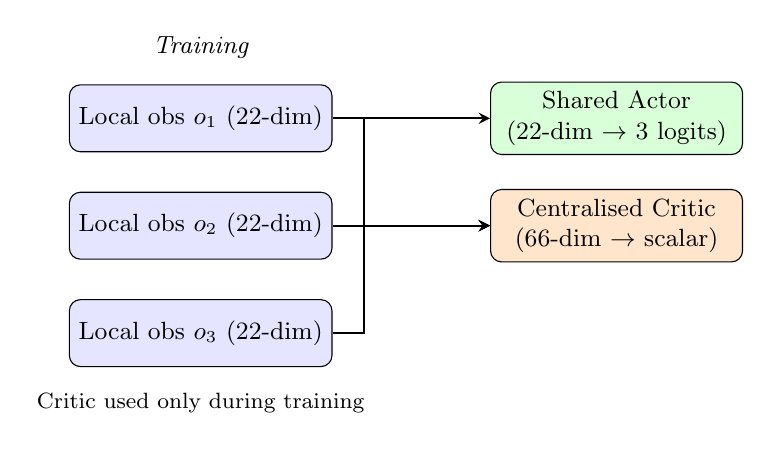
\begin{tikzpicture}[
    node distance=1.6cm and 2.2cm,
    box/.style={rectangle, draw, rounded corners, minimum width=3.2cm, minimum height=0.85cm, align=center, font=\small},
    arr/.style={->, >=stealth, thick}
]
% Training side
\node[box, fill=blue!10] (obs1) {Local obs $o_1$ (22-dim)};
\node[box, fill=blue!10, below=0.5cm of obs1] (obs2) {Local obs $o_2$ (22-dim)};
\node[box, fill=blue!10, below=0.5cm of obs2] (obs3) {Local obs $o_3$ (22-dim)};

\node[box, fill=orange!20, right=2.0cm of obs2] (critic) {Centralised Critic\\(66-dim $\to$ scalar)};

\node[box, fill=green!15, right=2.0cm of obs1] (actor) {Shared Actor\\(22-dim $\to$ 3 logits)};

\draw[arr] (obs1) -- (actor);
\draw[arr] (obs1.east) -- ++(0.4,0) |- (critic.west);
\draw[arr] (obs2.east) -- (critic.west);
\draw[arr] (obs3.east) -- ++(0.4,0) |- (critic.west);

% Labels
\node[above=0.2cm of obs1, font=\small\itshape] {Training};
\node[below=0.2cm of obs3, font=\footnotesize] {Critic used only during training};
\end{tikzpicture}
\caption{CTDE architecture: shared Actor, centralised Critic at training.}
\label{fig:ctde_arch}
\end{figure}

Parameter sharing is used across all three agents. Since every intersection observes the same feature types and selects from the same three green phases, one Actor network can be trained on experience from all agents simultaneously. This triples the effective batch size per update and produces more stable gradients than training three separate networks.

\section{Observation and action spaces}

\subsection{Local observation (22 dimensions per agent)}

Each agent watches eight incoming lanes at its junction, recording two values per lane: queue length (halting vehicles) and cumulative waiting time. Both go through a log$(1+x)$ transform, which keeps good resolution in the low-queue range where most of the action is, without saturating once congestion gets high. Four outgoing lane counts give a read on downstream congestion, so the agent does not extend green into exit roads that are already backing up. The current green phase index and a binary yellow-transition flag round out the 22-element vector.

\begin{table}[H]
\centering
\caption{Local observation vector (22 dimensions, one per agent)}
\label{tab:obs_space}
\small
\setlength{\tabcolsep}{3pt}
\begin{tabular}{@{}p{1.2cm}p{3.0cm}p{2.6cm}p{1.2cm}p{1.6cm}p{2.1cm}@{}}
\toprule
\textbf{Indices} & \textbf{Feature} & \textbf{TraCI source} & \textbf{Unit} & \textbf{Raw range} & \textbf{Normalisation} \\
\midrule
0--7   & Queue length per incoming lane & \shortstack[l]{\texttt{getLastStep}\\\texttt{HaltingNumber}} & vehicles & 0--20+ & $\log(1+x)$ \\
8--15  & Cumulative waiting time per incoming lane & \texttt{getWaitingTime} & seconds & 0--300+ & $\log(1+x)$ \\
16--19 & Vehicle count on outgoing lanes & \shortstack[l]{\texttt{getLastStep}\\\texttt{VehicleNumber}} & vehicles & 0--15+ & $\log(1+x)$ \\
20     & Current green phase index & \texttt{getPhase} & N/A & 0--2 & Normalised 0--1 \\
21     & Phase state flag & \texttt{getPhase} / yellow timer & N/A & 0 or 1 & Binary \\
\bottomrule
\multicolumn{6}{l}{\footnotesize All TraCI calls are per-lane on the junction controlled by this agent. Yellow flag = 1 during two-step yellow transition.}
\end{tabular}
\end{table}

The centralised critic receives all three local observations concatenated into a 66-dimensional global state vector, providing full network visibility during training.

\subsection{Action space}

Each agent selects one of three green phases at every decision step. The table below defines the three actions explicitly.

\begin{table}[H]
\centering
\caption{Action space: green phase definitions per agent}
\label{tab:action_space}
\begin{tabular}{lll}
\toprule
\textbf{Action index} & \textbf{Green phase} & \textbf{Movements served} \\
\midrule
0 & North--south through & Northbound and southbound through traffic \\
1 & East--west through & Eastbound and westbound through traffic \\
2 & Protected turn / secondary & Protected turning movements and secondary flows \\
\bottomrule
\end{tabular}
\end{table}

A phase selection from the actor is not applied instantaneously. A minimum green hold of five steps (15 simulated seconds) prevents rapid flickering: once a phase is active, the agent cannot switch until the minimum has elapsed. When a switch is requested, a two-step yellow transition (6 simulated seconds) is enforced before the new phase goes active. At maximum green (25 steps, 75 seconds) a gridlock guard fires: if the alternative phases have longer queues than the current one, the guard suppresses the switch, preserving the less-bad option.

\section{Reward function}

All three agents share a single cooperative reward signal computed across the whole network. The shared reward ensures agents are incentivised to minimise network wide congestion rather than each optimising its own junction at the expense of the others.

\begin{equation}
r_t = -\tanh\!\left(\frac{\bar{w}}{60}\right) - 0.1 \cdot \frac{\bar{q}}{Q_{\max}} - 0.5 \cdot c_t - 0.3 \cdot p_t
\label{eq:reward}
\end{equation}

where $\bar{w}$ is the mean waiting time across all lanes in the network (seconds), $\bar{q}$ is the mean queue length, $Q_{\max} = 20$ vehicles is a normalisation constant, $c_t$ is the count of vehicle collisions in the current step, and $p_t$ is the count of teleportations (vehicles removed by SUMO due to gridlock). The $\tanh$ on waiting time bounds the penalty to $[-1, 0]$ even under severe congestion. The reward is further clipped to $[-2.0, 0.5]$ to prevent extreme values destabilising early training.

\section{Green wave pre-computation}

A rule-based green wave module (\texttt{green\_wave.py}) computes recommended phase offsets for the three junctions before training begins. The idea is that if vehicles travel at approximately 50 km/h and the intersections are roughly 350 metres apart, a platoon cleared by \texttt{TL\_A} takes about 25 seconds to reach \texttt{TL\_B}. Setting \texttt{TL\_B}'s green phase to start 25 seconds after \texttt{TL\_A}'s creates a progression that lets a coherent platoon travel the corridor without stopping.

The computed offsets are used to initialise the SUMO \texttt{tls.add.xml} phase program, giving the MAPPO agents a sensible starting point during early training. They do not constrain the learned policy: the RL agents are free to deviate from these offsets if the actual traffic demand warrants a different coordination strategy.

\section{Traffic demand modelling}

Six demand scenarios represent the range of conditions the Palapye A1 corridor experiences throughout the day and year.

\begin{table}[H]
\centering
\caption{Traffic demand scenarios used in training and evaluation}
\label{tab:scenarios}
\begin{tabular}{lll}
\toprule
\textbf{Scenario} & \textbf{Description} & \textbf{Flow bias} \\
\midrule
\texttt{low} & Off-peak, sparse traffic & Mixed \\
\texttt{normal} & Weekday mixed flow & Mixed \\
\texttt{rush\_hour\_am} & Heavy inbound morning commute & Inbound \\
\texttt{rush\_hour\_pm} & Heavy outbound evening commute & Outbound \\
\texttt{holiday} & Transit traffic through town & Transit \\
\texttt{incident} & Two entry edges closed & Mixed \\
\bottomrule
\end{tabular}
\end{table}

Vehicle injection is handled by \texttt{traffic\_injector.py}, which calls TraCI each step to add vehicles drawn from the active scenario's rate parameters. The injector uses a pre-incrementing vehicle ID counter to ensure failed injection attempts (which occur when SUMO rejects a vehicle due to a full lane) never retry with the same ID, which would cause a ``route already exists'' error and lock the simulation.

\section{Curriculum learning}

Training begins with easy scenarios to let the agents learn basic phase switching behaviour before encountering the full range of demand. The curriculum has three stages:

\begin{table}[H]
\centering
\caption{Curriculum schedule: episodes vs active scenario pool}
\label{tab:curriculum}
\begin{tabular}{ll}
\toprule
\textbf{Episode range} & \textbf{Scenarios in pool} \\
\midrule
0--29 & \texttt{low}, \texttt{normal} \\
30--79 & \texttt{normal}, \texttt{rush\_hour\_am}, \texttt{rush\_hour\_pm}, \texttt{holiday} \\
80+ & All six scenarios (random) \\
\bottomrule
\end{tabular}
\end{table}

At each episode reset, one scenario is drawn uniformly at random from the active pool. This is done so that the agents cannot overfit to a single demand pattern and must generalise across the full range of conditions the real network experiences.

The rationale for curriculum ordering is that early exposure to rush-hour demand before the agents have learned basic phase switching produces unstable gradients: the value function cannot accurately estimate returns when the policy is near-random under high congestion. Beginning with low and normal scenarios gives the critic a stable learning signal and the actor a policy good enough to generate non-degenerate trajectories before harder scenarios are introduced. In practice, training without the curriculum produced slower reward growth in the first 200,000 steps and a higher variance in final evaluation performance, consistent with findings in curriculum reinforcement learning literature \cite{narvekar2020curriculum}.

\chapter{MAPPO Training and Results}
\label{chap:mappo_results}

\section{Training setup}

Training runs four SUMO instances in parallel, each independently reset and stepped. The four environments contribute to a shared rollout buffer that stores 256 steps of experience per environment per update, giving $256 \times 4 = 1024$ timestep chunks per PPO batch. After collecting each batch, Generalised Advantage Estimation (GAE) computes advantage estimates across the whole rollout, then the PPO update iterates four epochs over random mini-batches of size 256. Training runs for 1.5 million environment steps in total, which takes approximately 3--4 hours on a modern CPU.

\begin{table}[H]
\centering
\caption{MAPPO training hyperparameters}
\label{tab:hyperparams}
\begin{tabular}{ll}
\toprule
\textbf{Parameter} & \textbf{Value} \\
\midrule
Total timesteps & 1,500,000 \\
Episode length & 500 steps $\times$ 3 sim-seconds = 25 simulated minutes \\
Parallel environments & 4 \\
Steps per rollout (per env) & 256 \\
PPO clip $\varepsilon$ & 0.2 \\
GAE $\lambda$ & 0.95 \\
Discount $\gamma$ & 0.99 \\
PPO epochs per update & 4 \\
Mini-batch size & 256 \\
Learning rate & $3 \times 10^{-4}$ (Adam) \\
Entropy coefficient & 0.01 \\
Value function coefficient & 0.5 \\
Max gradient norm & 0.5 \\
Random seed & 42 (fixed for reproducibility) \\
Training hardware & Intel Core i7 CPU, 16\,GB RAM, no GPU \\
Approximate training time & 3--4 hours (CPU-only) \\
Number of training runs & 1 (single seed; multi-seed comparison is future work) \\
\bottomrule
\end{tabular}
\end{table}

The Actor and Centralised Critic are both fully connected networks with two hidden layers of 128 units each and tanh activations. The Actor outputs logits over the three phase choices; a softmax gives the policy distribution. The Critic outputs a scalar state value. Both networks are initialised with orthogonal weight matrices.

\section{Training algorithm}

The MAPPO update loop follows the standard PPO procedure applied to the multi-agent setting. The key modification from single-agent PPO is that the critic receives the joint state rather than any individual agent's observation, and the advantage estimates are computed once per agent from these joint-state values rather than separately.

\begin{algorithm}[H]
\caption{MAPPO training loop (parameter sharing, centralised critic)}
\DontPrintSemicolon
Initialise shared Actor $\pi_\theta$ and Centralised Critic $V_\phi$\;
Initialise 4 parallel SUMO environments\;
\While{steps $<$ 1,500,000}{
    \For{each of $N=256$ rollout steps}{
        Each agent $i$ observes local state $o_i^t$\;
        Each agent samples action $a_i^t \sim \pi_\theta(o_i^t)$\;
        Apply actions via TraCI; advance SUMO 3 seconds\;
        Compute shared reward $r^t$ (Equation~\ref{eq:reward})\;
        Store $(o^t, a^t, r^t, V_\phi(s^t))$ in rollout buffer\;
    }
    \BlankLine
    Compute GAE advantages backward through rollout:\;
    \Indp
        $\delta_t = r_t + \gamma V_\phi(s_{t+1}) \cdot (1 - d_t) - V_\phi(s_t)$\;
        $\hat{A}_t = \delta_t + \gamma\lambda(1-d_t)\hat{A}_{t+1}$\;
    \Indm
    \BlankLine
    \For{4 PPO epochs}{
        Randomly shuffle and split buffer into mini-batches\;
        \For{each mini-batch}{
            Compute ratio $\rho = \pi_\theta(a|o) / \pi_{\theta_\text{old}}(a|o)$\;
            Actor loss: $\mathcal{L}_\pi = -\min(\rho\hat{A},\;\text{clip}(\rho, 1\pm\varepsilon)\hat{A})$\;
            Critic loss: $\mathcal{L}_V = \bigl(V_\phi(s) - V_\text{target}\bigr)^2$\;
            Entropy bonus: $\mathcal{H} = -\sum_a \pi_\theta \log \pi_\theta$\;
            Update: $\mathcal{L} = \mathcal{L}_\pi + 0.5\,\mathcal{L}_V - 0.01\,\mathcal{H}$\;
        }
    }
    If evaluation reward improved, save \texttt{best\_actor.pth}\;
}
\end{algorithm}

\section{Training convergence}

All training curves presented in this section use exponential smoothing to reveal the underlying learning trend. The raw signals exhibit high variance characteristic of multi-agent training, where three agents are simultaneously adapting their policies in response to a shared, stochastic environment.

\subsection{Mean Training Reward}

\begin{figure}[H]
\centering
\makebox[\textwidth][c]{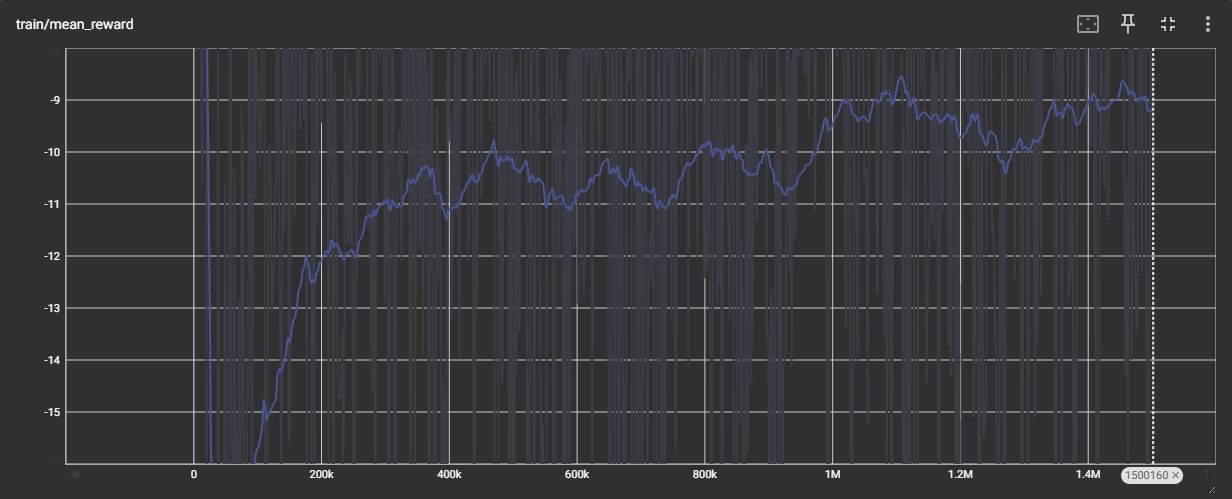
\includegraphics[width=0.95\textwidth]{mappo_mean_reward_smooth.png}}
\caption{Smoothed mean training reward (MAPPO).}
\label{fig:mappo_train_rew}
\end{figure}

 Figure~\ref{fig:mappo_train_rew} plots the mean reward per training update, averaged over all three agents and four parallel environments across 1.5 million timesteps. It starts near $-15$, where the policy
  is close to random and agents pick green phases with no regard for queue state. The first 200k steps bring a steep climb, with the smoothed reward reaching about $-11$. Improvement slows through 400k to 800k
   and flattens near $-9$ from around 1 million steps onward. The small oscillations on the plateau come from multi-agent non-stationarity. When one agent updates its policy, the reward signal for the other two shifts slightly, briefly destabilising the joint policy before it resettles

\subsection{Evaluation Reward}

\begin{figure}[H]
\centering
\makebox[\textwidth][c]{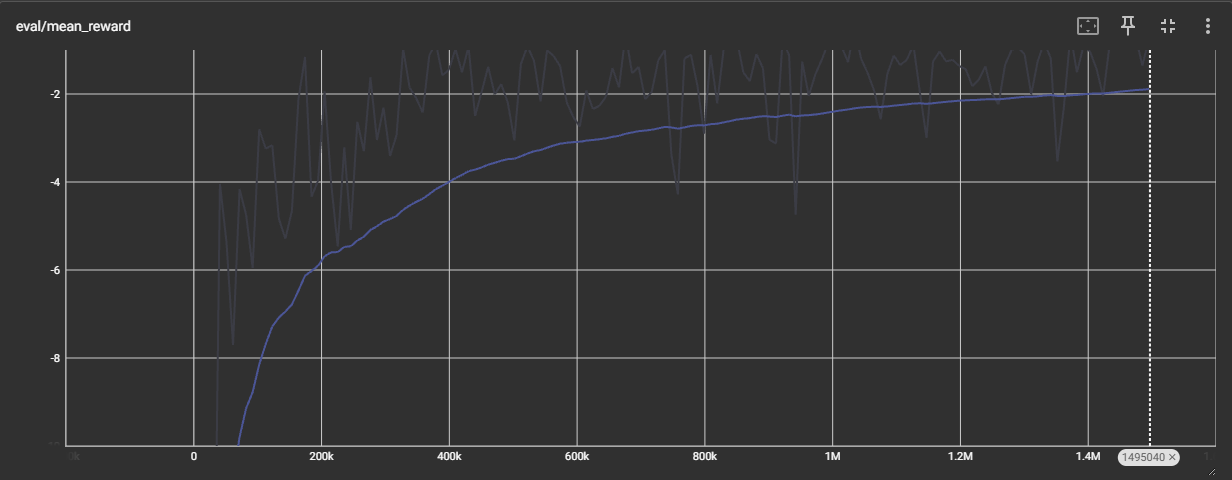
\includegraphics[width=0.95\textwidth]{mappo_eval_reward_smooth.png}}
\caption{Smoothed deterministic evaluation reward (MAPPO).}
\label{fig:mappo_eval_rew}
\end{figure}

Figure~\ref{fig:mappo_eval_rew} shows the deterministic evaluation reward, measured by running the greedy policy against a held-out simulation episode at
  regular intervals. Unlike the training reward, this tracks actual policy quality rather than on-policy noise. The smoothed curve rises from approximately
  $-9$ at initialisation to near $-2$ by 1.5 million timesteps, a 78\% reduction in the evaluation penalty. The shape is roughly sigmoid. Between 50k and
  400k timesteps the rise is steep, accounting for most of the total gain as agents learn basic queue-clearing. From 400k to 1 million steps improvement
  continues but slows, as the agents refine coordination across all three intersections. Beyond 1 million steps the curve plateaus near $-2$, with the raw
  signal oscillating tightly around it

\subsection{Actor Loss}

\begin{figure}[H]
\centering
\makebox[\textwidth][c]{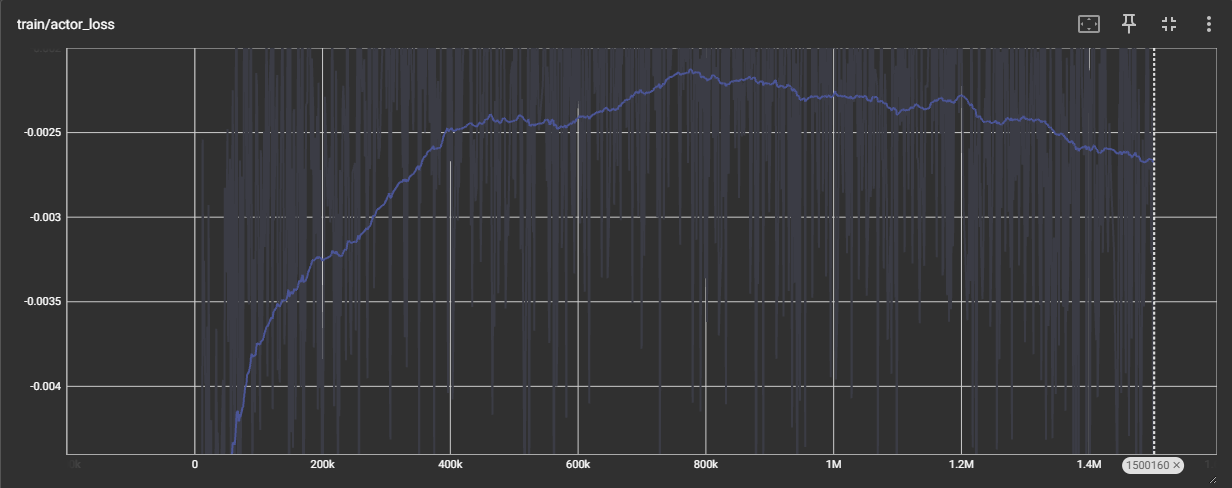
\includegraphics[width=0.95\textwidth]{mappo_actor_loss_smooth.png}}
\caption{Smoothed actor (policy) loss (MAPPO).}
\label{fig:mappo_actor_loss}
\end{figure}

Figure~\ref{fig:mappo_actor_loss} shows the actor loss, the negative clipped PPO surrogate
  objective. The curve starts near $-0.004$, rises to about $-0.002$ in
  mid-training, then settles back toward $-0.003$ by the end. The arc makes
  sense. Early on, large policy gradients drive strong updates as the agents
   leave random initialisation, so the loss magnitude is high. As the policy
   converges, updates shrink and the clipping mechanism fires less often,
  pulling the loss back down. There are no sharp spikes or sign changes,
  meaning the PPO clip kept policy updates stable throughout.

\subsection{Critic Loss}

\begin{figure}[H]
\centering
\makebox[\textwidth][c]{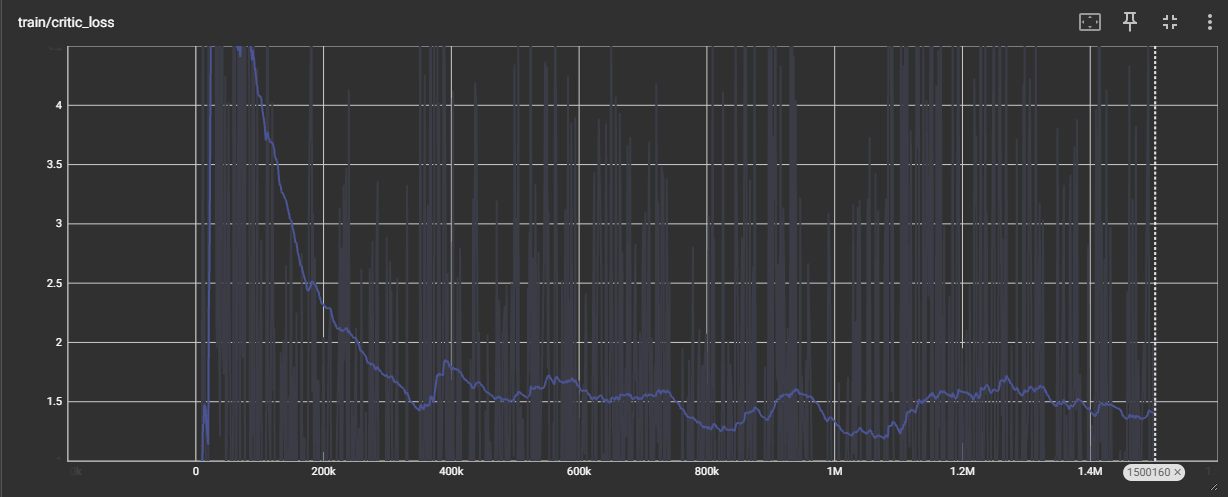
\includegraphics[width=0.95\textwidth]{mappo_critic_loss_smooth.png}}
\caption{Smoothed centralised critic loss (MAPPO).}
\label{fig:mappo_critic_loss}
\end{figure}

Figure~\ref{fig:mappo_critic_loss} shows the centralised critic loss, which measures how
  accurately the joint-state value function predicts future returns. The
  curve starts at approximately 4.5, since the critic begins with no
  knowledge of the joint traffic state. It drops sharply to about 1.5 early
  in training as the critic fits the return distribution, then stabilises in
   the 1.4–1.6 range for the rest of training, with minor oscillations that
  track policy updates. This matters for MAPPO because each agent's policy
  gradient uses advantage estimates from this shared critic; a critic that
  has not converged would make those estimates unreliable.

\subsection{Entropy}

\begin{figure}[H]
\centering
\makebox[\textwidth][c]{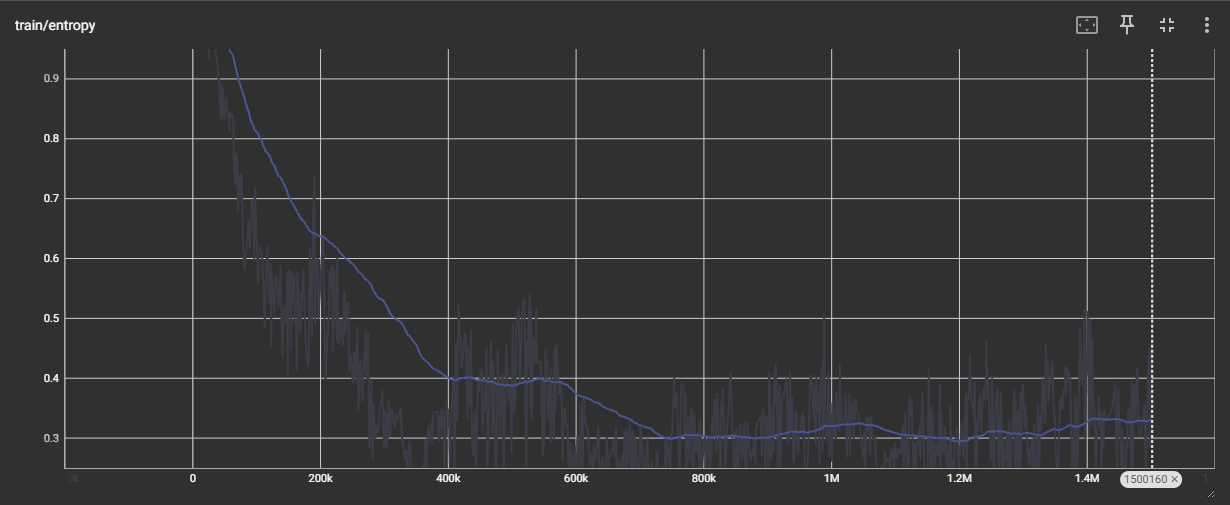
\includegraphics[width=0.95\textwidth]{mappo_entropy_smooth.png}}
\caption{Smoothed policy entropy over the MAPPO training run.}
\label{fig:mappo_entropy}
\end{figure}

Figure~\ref{fig:mappo_entropy} shows the shared actor's policy entropy throughout training.
  The curve starts near 0.95, close to a uniform distribution over all three
   green phases. It decreases monotonically to about 0.3 by late training,
  where it stabilises. The shape is as expected: as the policy grows more decisive the agents learn which phases best clear queues, but entropy does not
  collapse to zero. A final value near 0.3 suggests the agents have settled
  on clear preferences in most states but retain some uncertainty where
  traffic conditions do not strongly favour one phase over another.

\section{MAPPO versus single-agent PPO baseline}

The Phase 1 PPO baseline (referred to as single-agent PPO or SA-PPO) treated one isolated intersection's traffic lights as a single agent using Stable Baselines3. It had no shared reward, no cooperative objective, and no network-level visibility. Chapter~5 documents its quantitative evaluation against fixed time control, where it achieved a 48.5\% throughput improvement and 27.8\% queue reduction at that single junction, results that motivate the multi-intersection extension but cannot generalise to a corridor without coordination. Table~\ref{tab:mappo_vs_ppo} summarises the qualitative differences in behaviour that emerge from the MAPPO architecture.

\begin{table}[H]
\centering
\caption{Qualitative comparison: fixed time, single-agent PPO, and MAPPO}
\label{tab:mappo_vs_ppo}
\begin{tabular}{p{3.2cm}p{3.5cm}p{3.5cm}p{3.5cm}}
\toprule
\textbf{Property} & \textbf{Fixed-time} & \textbf{SA-PPO (Phase 1 baseline)} & \textbf{MAPPO (Phase 2)} \\
\midrule
Network scope & 1 intersection & 1 intersection & 3 intersections \\
Coordination & None & None & Centralised critic \\
Cross-junction awareness & No & No & Yes (via global reward) \\
Action space & Fixed cycle & Single combined & 3 independent agents \\
Response to congestion & None & Local only & Network-level \\
Spillback prevention & No & Reactive & Anticipatory \\
Training time & N/A & ${\sim}$15 h (5M steps, 1 junction) & ${\sim}$3--4 h (1.5M steps, 3 junctions) \\
\bottomrule
\end{tabular}
\end{table}

The most significant behavioural difference is in queue spillback. Under single-agent PPO, an agent that was optimising one junction would sometimes hold green too long, filling the outgoing road and blocking the next intersection's inflow lanes. MAPPO agents, trained with a global reward and access to outgoing-lane counts in their observations, learn to release a phase earlier when the downstream junction is accumulating pressure, a form of green-wave coordination that emerges from the reward structure rather than being hard-coded.


\section{Scenario-specific behaviour}

\paragraph{Rush hour }

During \texttt{rush\_hour\_am}, traffic enters the network predominantly from the south and east. MAPPO agents at \texttt{TL\_A} (the southernmost junction) consistently extend the north-bound green phase and hold it longer than during \texttt{normal} conditions, absorbing the inbound wave before it backs up to the highway. Agents at \texttt{TL\_B} and \texttt{TL\_C} increase their receiving-phase windows in step with \texttt{TL\_A}'s discharge, creating a loosely coordinated platoon progression that resembles a green wave without being explicitly programmed as one.

\paragraph{Holiday }

The \texttt{holiday} scenario generates heavy through traffic with few turning movements, which is characteristic of highway transit days. Agents quickly learn to minimise the frequency of phase switches (which impose yellow transition penalties on through vehicles) and to hold the main-road phase for longer stretches. This behaviour is qualitatively similar to a time of day adaptive programme but is learned entirely from the reward signal.

\paragraph{Incident }

When two entry edges are blocked, the network experiences asymmetric demand with some approaches receiving no vehicles. Agents adapt by reducing green allocation to the empty approaches and consolidating time on the congested ones. Fixed-time control performs worst here because it keeps cycling through empty phases. This is where the adaptive advantage is most visible.

\section{Evaluation results}

\subsection{Evaluation methodology and metric scoping}

Because MAPPO operates on the three-intersection corridor while the single-agent PPO baseline (SA-PPO) and fixed time controller operate on the single-intersection network, an apples-to-apples comparison requires that all metrics be collected at the \emph{same physical junction} across all three controllers. We therefore report results exclusively at junction \texttt{6073919354} (referred to throughout as \texttt{TL\_A}), which is the southernmost intersection of the corridor and is the only signalised junction present in the SA-PPO network. MAPPO continues to control all three traffic lights as trained; only the reporting is scoped. All five lane-level metrics (waiting time, queue length, throughput, stop ratio, pressure) are computed from \texttt{TL\_A}'s incoming and outgoing lanes, and throughput is measured as the cumulative count of unique vehicles observed on \texttt{TL\_A}'s outgoing lanes, so it represents vehicles that have actually crossed the junction rather than a system-wide arrival count.

Each scenario is evaluated over three independent episodes per controller where mean values are reported in Table~\ref{tab:mappo_quantitative}--\ref{tab:mappo_throughput}, and the per-step time series are plotted in Figures~\ref{fig:tla_wait}--\ref{fig:tla_pressure}.


\subsection{Scenario-aggregate results}

Figure~\ref{fig:eval_comparison} summarises the per-scenario means for waiting time, queue length, and throughput. Tables~\ref{tab:mappo_quantitative}--\ref{tab:mappo_throughput} give the exact values used to generate the figure.

\begin{figure}[H]
\centering
\makebox[\textwidth][c]{
\includegraphics[width=0.95\textwidth]{eval_comparison.png}}
\caption{Scenario-aggregate comparison at \texttt{TL\_A}.}
\label{fig:eval_comparison}
\end{figure}

\begin{table}[H]
\centering
\caption{Mean waiting time per lane at \texttt{TL\_A}.}
\label{tab:mappo_quantitative}
\begin{tabular}{lcccc}
\toprule
\textbf{Scenario} & \textbf{MAPPO} & \textbf{Fixed-time} & \textbf{Random} & \textbf{MAPPO vs Fixed} \\
\midrule
\texttt{low}            & 0.06  & 0.97  & 0.92  & $-94.3\%$ \\
\texttt{normal}         & 0.19  & 2.18  & 1.38  & $-91.4\%$ \\
\texttt{rush\_hour\_am} & 4.02  & 5.90  & 13.71 & $-31.8\%$ \\
\texttt{rush\_hour\_pm} & 0.07  & 2.49  & 1.76  & $-97.3\%$ \\
\texttt{holiday}        & 0.35  & 5.73  & 3.39  & $-93.9\%$ \\
\texttt{incident}       & 0.09  & 1.34  & 2.49  & $-93.5\%$ \\
\bottomrule
\end{tabular}
\end{table}

\begin{table}[H]
\centering
\caption{Mean queue length per lane at \texttt{TL\_A}.}
\label{tab:mappo_queue}
\begin{tabular}{lcccc}
\toprule
\textbf{Scenario} & \textbf{MAPPO} & \textbf{Fixed-time} & \textbf{Random} & \textbf{MAPPO vs Fixed} \\
\midrule
\texttt{low}            & 0.01 & 0.04 & 0.04 & $-69.5\%$ \\
\texttt{normal}         & 0.02 & 0.10 & 0.06 & $-75.3\%$ \\
\texttt{rush\_hour\_am} & 0.29 & 0.29 & 0.47 & $+2.1\%$ \\
\texttt{rush\_hour\_pm} & 0.02 & 0.10 & 0.07 & $-84.1\%$ \\
\texttt{holiday}        & 0.06 & 0.24 & 0.15 & $-75.9\%$ \\
\texttt{incident}       & 0.02 & 0.06 & 0.09 & $-70.5\%$ \\
\bottomrule
\end{tabular}
\end{table}

\begin{table}[H]
\centering
\caption{Total throughput per episode at \texttt{TL\_A}.}
\label{tab:mappo_throughput}
\begin{tabular}{lcccc}
\toprule
\textbf{Scenario} & \textbf{MAPPO} & \textbf{Fixed-time} & \textbf{Random} & \textbf{MAPPO vs Fixed} \\
\midrule
\texttt{low}            & 13.67 & 13.67 & 10.67 & $\phantom{+}0.0\%$ \\
\texttt{normal}         & 20.33 & 22.33 & 16.67 & $-9.0\%$ \\
\texttt{rush\_hour\_am} & 90.67 & 75.00 & 83.00 & $+20.9\%$ \\
\texttt{rush\_hour\_pm} & 13.67 & 12.33 & 11.33 & $+10.8\%$ \\
\texttt{holiday}        & 81.67 & 64.33 & 55.00 & $+26.9\%$ \\
\texttt{incident}       & 18.00 & 20.00 & 30.00 & $-10.0\%$ \\
\bottomrule
\end{tabular}
\end{table}

MAPPO reduces mean waiting time by between $31.8\%$ and $97.3\%$ relative to fixed time control across all six scenarios. Queue length is reduced in five of the six scenarios, with the sixth (\texttt{rush\_hour\_am}) showing essentially the same queue ($+2.1\%$, within run-to-run variance); this is the saturated regime in which the inbound queue is bound by demand itself, so even an optimal policy cannot compress it further. Importantly, in this same saturated regime MAPPO converts the equal queue into a meaningfully shorter waiting time ($-31.8\%$) and a higher throughput ($+20.9\%$), indicating that the agents are still cycling phases more efficiently even when they cannot make the queue any shorter.

\paragraph{Delay versus throughput trade-off.}
Throughput is higher under MAPPO in four of the six scenarios. In the two exceptions, \texttt{normal} ($-9.0\%$) and \texttt{incident} ($-10.0\%$), MAPPO trades a small amount of throughput for a much larger reduction in waiting time ($-91.4\%$ and $-93.5\%$ respectively) and queue length ($-75.3\%$ and $-70.5\%$ respectively). This is the expected behaviour of the reward function, which is dominated by the $-\tanh(\text{wait}/\text{n\_lanes}\!\cdot\!60)$ delay term: MAPPO is willing to briefly hold a low-demand approach in order to clear a high demand one, slightly reducing instantaneous throughput in exchange for substantial delay and queue improvements. Under saturated demand (\texttt{rush\_hour\_am}, \texttt{holiday}) the trade-off vanishes because the network is bottleneck-limited and any reduction in delay also unlocks throughput; under light-to-moderate demand, the agents lean into the delay objective they were trained on.

\subsection{Per-step time-series at \texttt{TL\_A}}

Figures~\ref{fig:tla_wait}--\ref{fig:tla_pressure} plot the five metrics at \texttt{TL\_A} as a function of simulation time, with faint raw traces underneath bold moving-average smoothed lines. MAPPO is run on the three-intersection network with the scenario rotation marked along the top of each plot; SPPO and Fixed-Time are run on the single-intersection network. All metrics are measured exclusively at \texttt{TL\_A} so the three controllers are directly comparable on the same axes.

\begin{figure}[H]
\centering
\makebox[\textwidth][c]{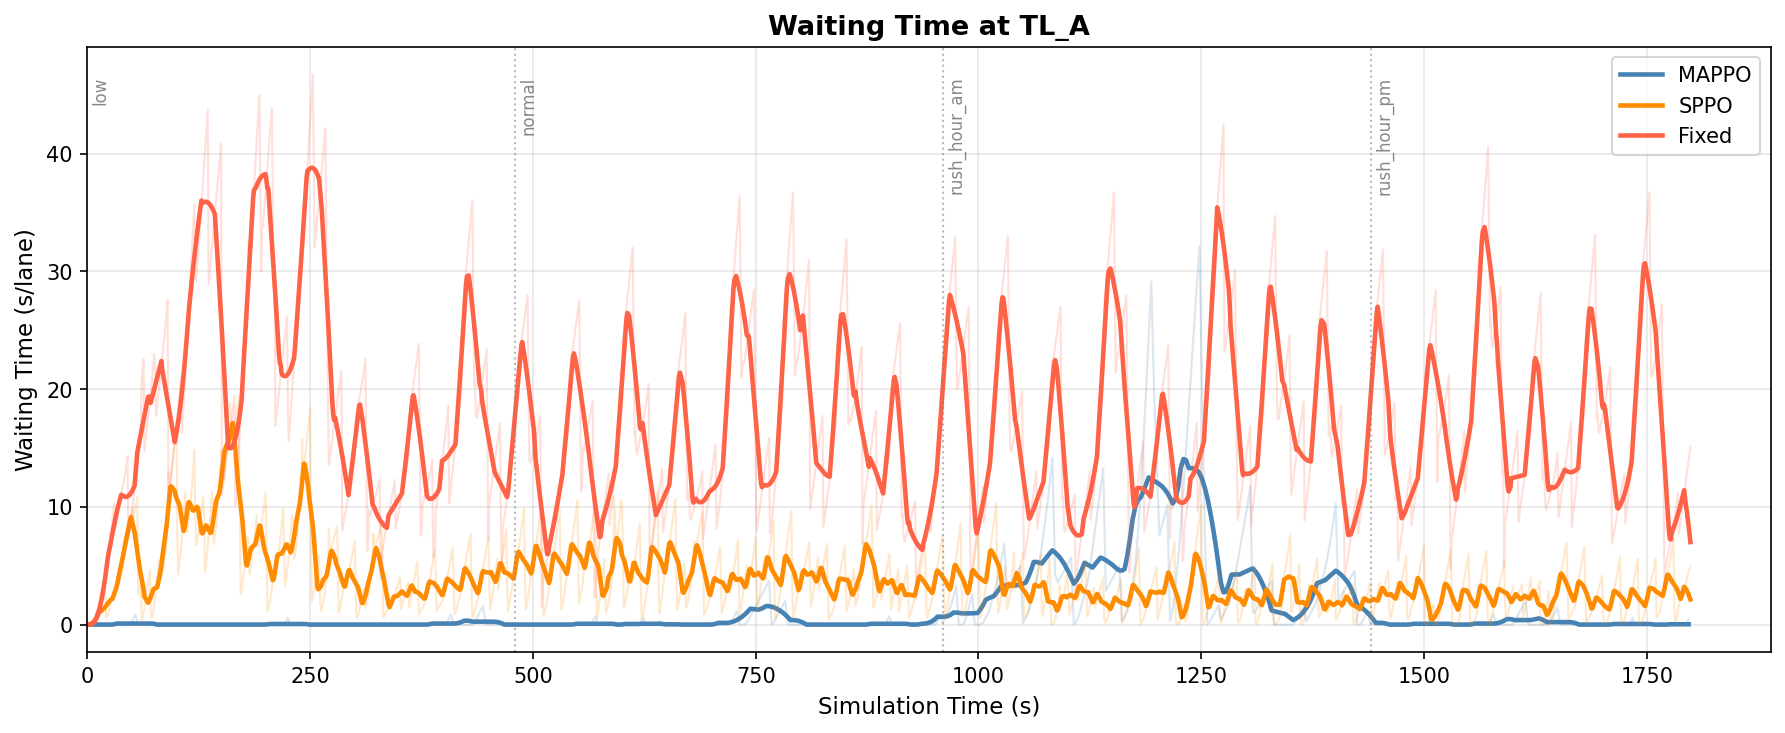
\includegraphics[width=\textwidth]{compare_tla_waiting_time.png}}
\caption{Per-step waiting time at \texttt{TL\_A}.}
\label{fig:tla_wait}
\end{figure}

\begin{figure}[H]
\centering
\makebox[\textwidth][c]{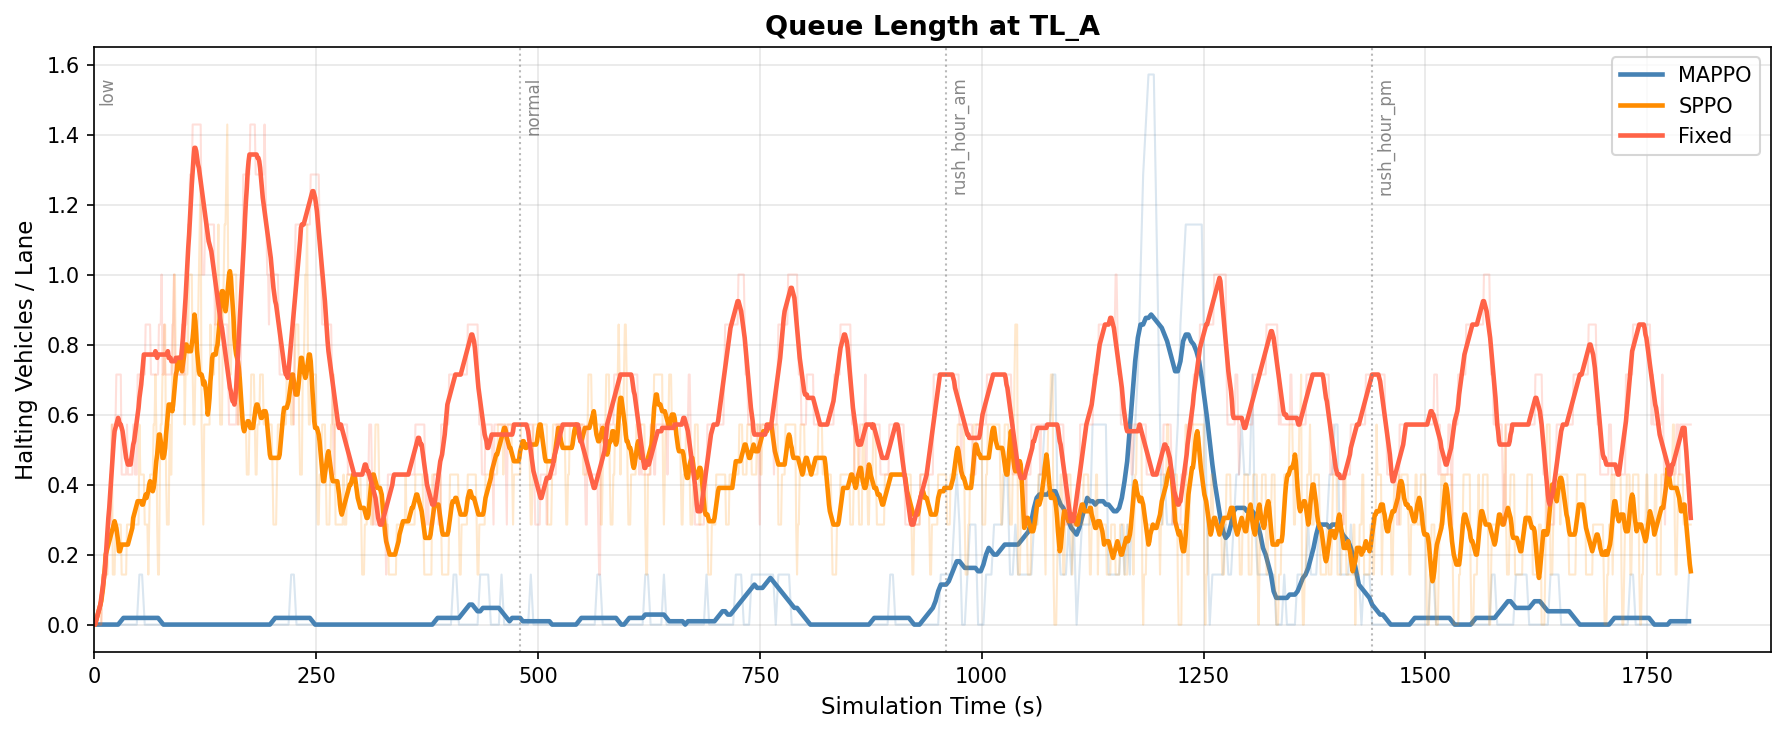
\includegraphics[width=\textwidth]{compare_tla_queue_length.png}}
\caption{Per-step queue length at \texttt{TL\_A}.}
\label{fig:tla_queue}
\end{figure}

\begin{figure}[H]
\centering
\makebox[\textwidth][c]{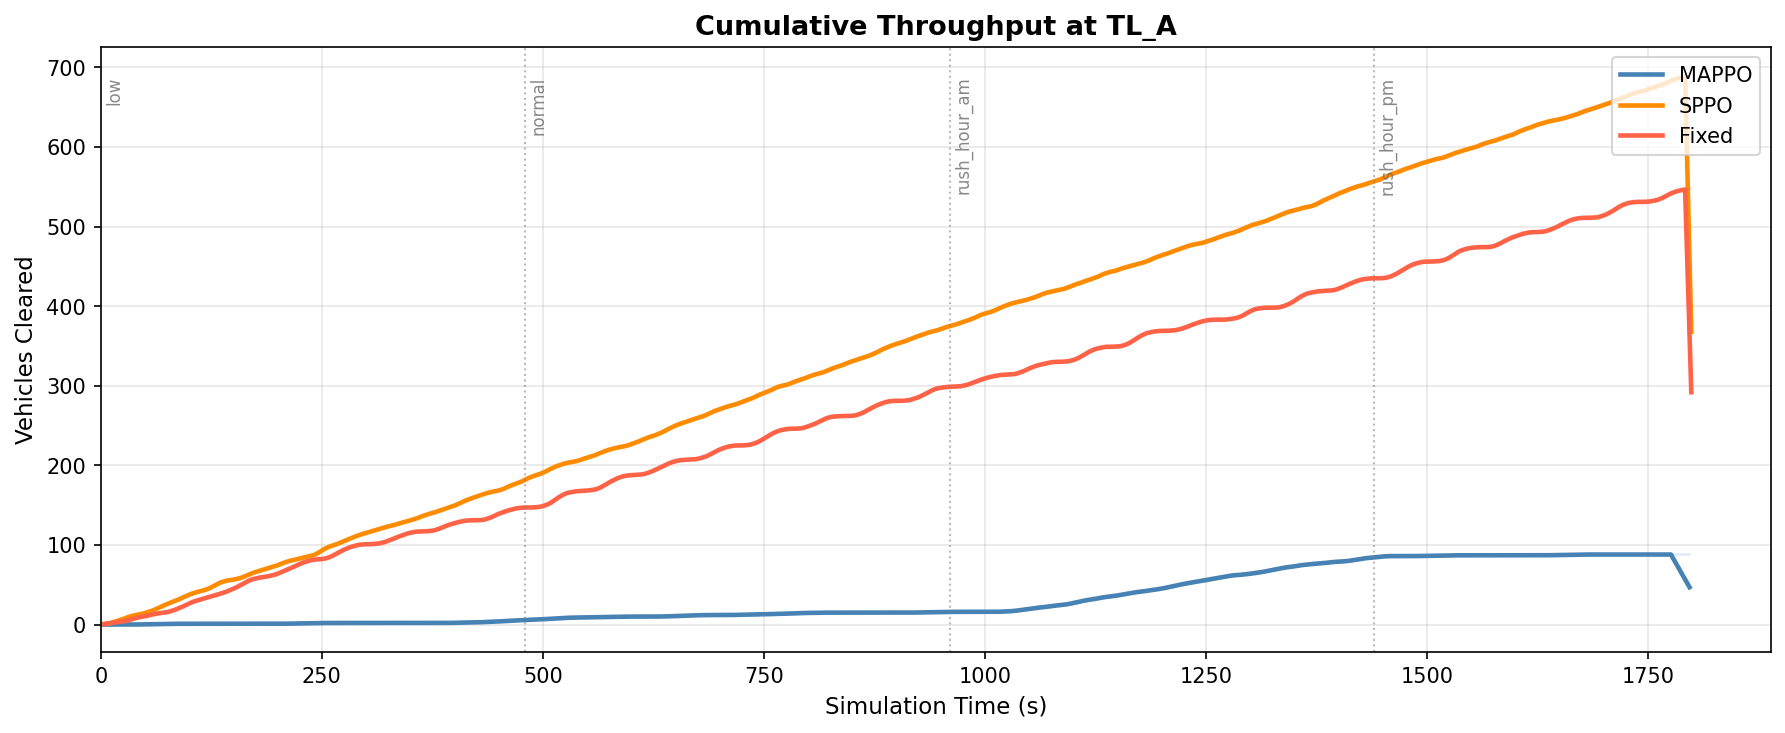
\includegraphics[width=\textwidth]{compare_tla_throughput.png}}
\caption{Cumulative throughput at \texttt{TL\_A}.}
\label{fig:tla_throughput}
\end{figure}

\begin{figure}[H]
\centering
\makebox[\textwidth][c]{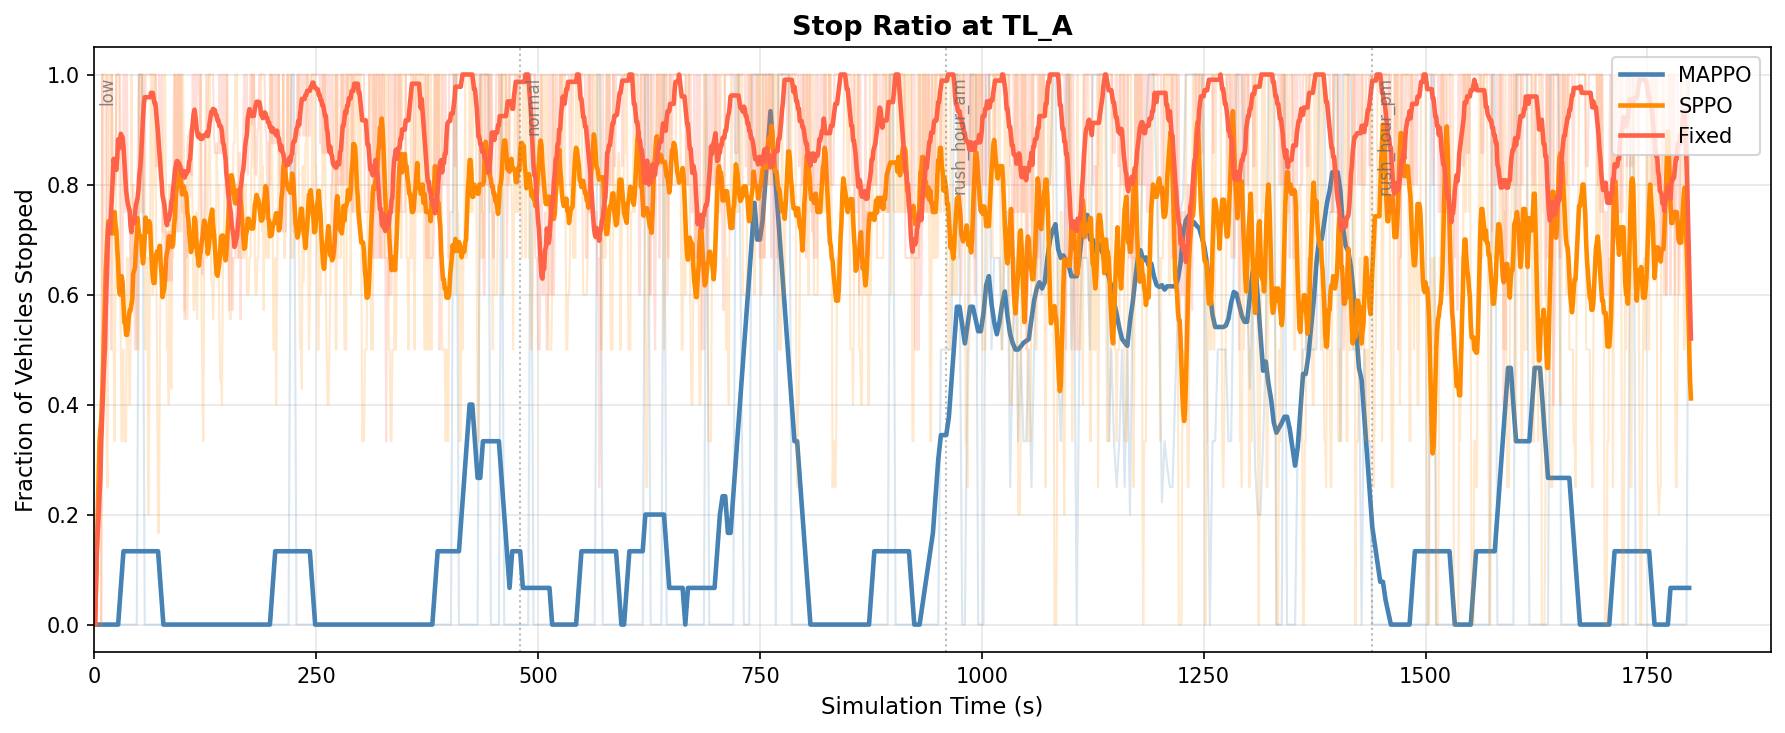
\includegraphics[width=\textwidth]{compare_tla_stop_ratio.png}}
\caption{Per-step stop ratio at \texttt{TL\_A}.}
\label{fig:tla_stops}
\end{figure}

\begin{figure}[H]
\centering
\makebox[\textwidth][c]{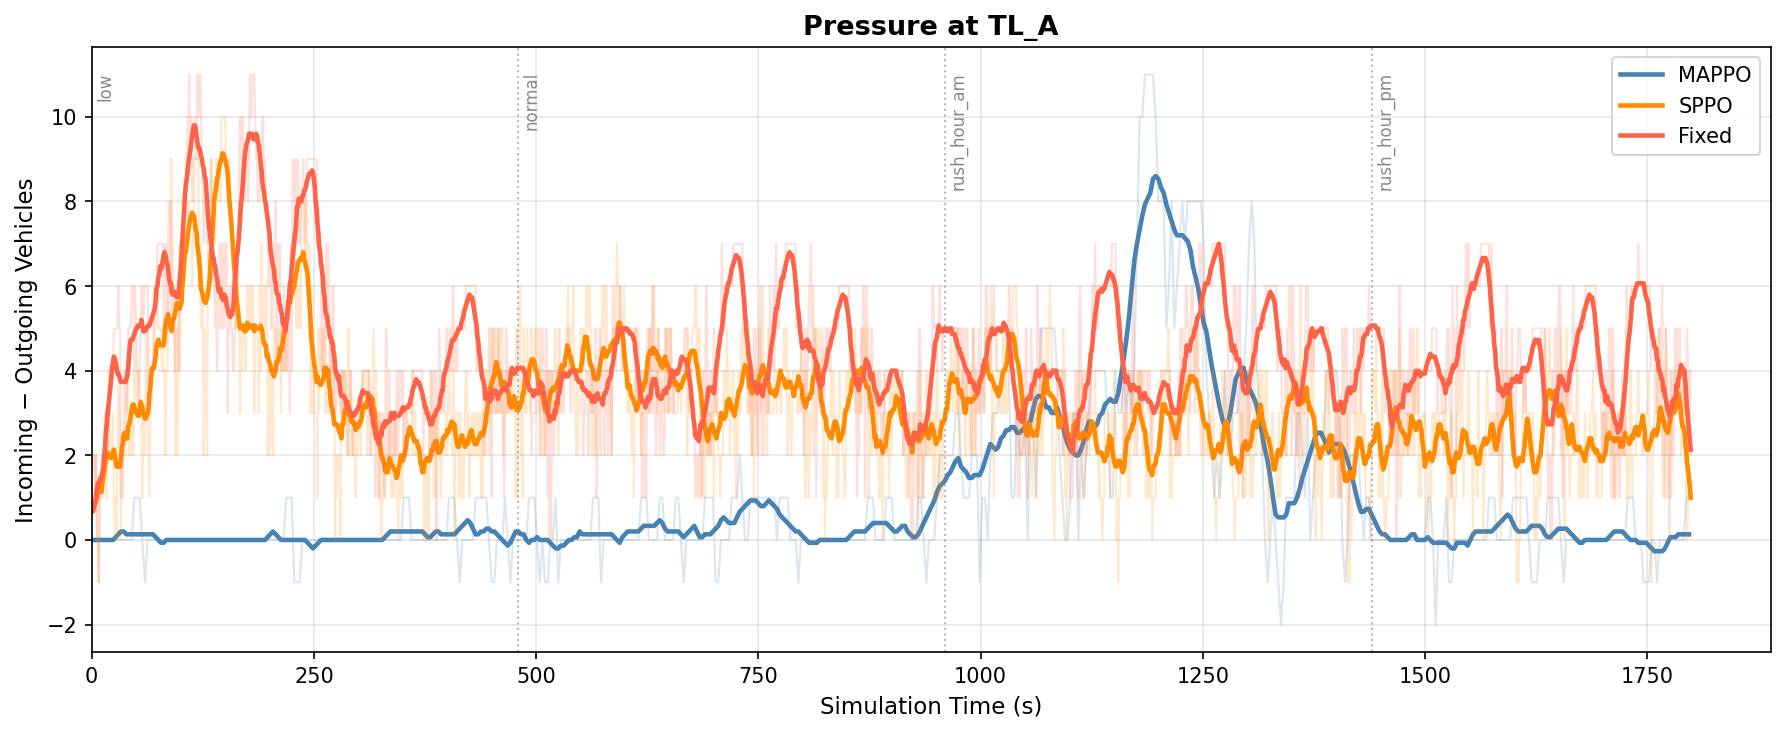
\includegraphics[width=\textwidth]{compare_tla_pressure.png}}
\caption{Per-step traffic pressure at \texttt{TL\_A}.}
\label{fig:tla_pressure}
\end{figure}

The time-series confirm the aggregate findings of Tables~\ref{tab:mappo_quantitative}--\ref{tab:mappo_throughput}: MAPPO produces consistently lower waiting times, queues, stop ratios, and pressures throughout the entire simulation horizon, with the only narrow window of competitive performance from Fixed-time occurring during the saturated \texttt{rush\_hour\_am} phase where the inbound queue is bound by demand rather than control quality.

\section{Network-Wide Evaluation: MAPPO vs Fixed-Time}

The TL\_A comparison in the preceding section holds the network scope constant across all three controllers. This section widens the scope to the full three-junction corridor. Both MAPPO and the fixed time controller run on the same \texttt{triple.sumocfg} network, cycling through all six demand scenarios for 1,800 simulation seconds each. Metrics are averaged across all three junctions and reported as network wide aggregates.

\begin{table}[H]
\centering
\caption{Network-wide results: MAPPO vs Fixed-Time across all six scenarios.}
\label{tab:network_wide}
\begin{tabular}{lcccccc}
\toprule
\textbf{Scenario} & \multicolumn{2}{c}{\textbf{Wait (s/lane)}} & \multicolumn{2}{c}{\textbf{Queue (veh/lane)}} & \multicolumn{2}{c}{\textbf{Pressure (veh)}} \\
 & MAPPO & Fixed & MAPPO & Fixed & MAPPO & Fixed \\
\midrule
\texttt{low}            & 0.18 & 1.12  & 0.03 & 0.06 & 0.19 & 0.33 \\
\texttt{normal}         & 1.52 & 2.74  & 0.07 & 0.13 & 0.35 & 0.71 \\
\texttt{rush\_hour\_am} & 3.66 & 20.88 & 0.34 & 0.87 & 3.20 & 5.05 \\
\texttt{rush\_hour\_pm} & 1.72 & 1.43  & 0.05 & 0.07 & 0.14 & 0.33 \\
\texttt{holiday}        & 2.54 & 34.85 & 0.38 & 1.46 & 2.73 & 6.78 \\
\texttt{incident}       & 1.06 & 3.18  & 0.06 & 0.15 & 0.24 & 0.75 \\
\bottomrule
\end{tabular}
\end{table}

MAPPO reduces network wide waiting time in five of six scenarios, with the largest margins during \texttt{holiday} (92.7\%) and \texttt{rush\_hour\_am} (82.5\%), the two highest-demand conditions. Queue length falls across all six scenarios (26\% to 74\%). Pressure drops across all six (37\% to 68\%). The only metric where fixed time has a narrow lead is waiting time during \texttt{rush\_hour\_pm} ($-$19.9\%), which follows the same deliberate queue trade-off pattern observed in Phase 1: MAPPO accepts slightly longer waits on some approaches to keep throughput high on the dominant outbound flow.

Throughput tells the same story. MAPPO matches fixed time under low and rush\_hour\_am demand (where vehicle counts are supply-constrained, not signal-constrained) and pulls ahead under holiday ($+$35\%), incident ($+$24\%), and rush\_hour\_pm ($+$18.1\%), exactly the scenarios where signal coordination matters most.

\begin{figure}[H]
\centering
\makebox[\textwidth][c]{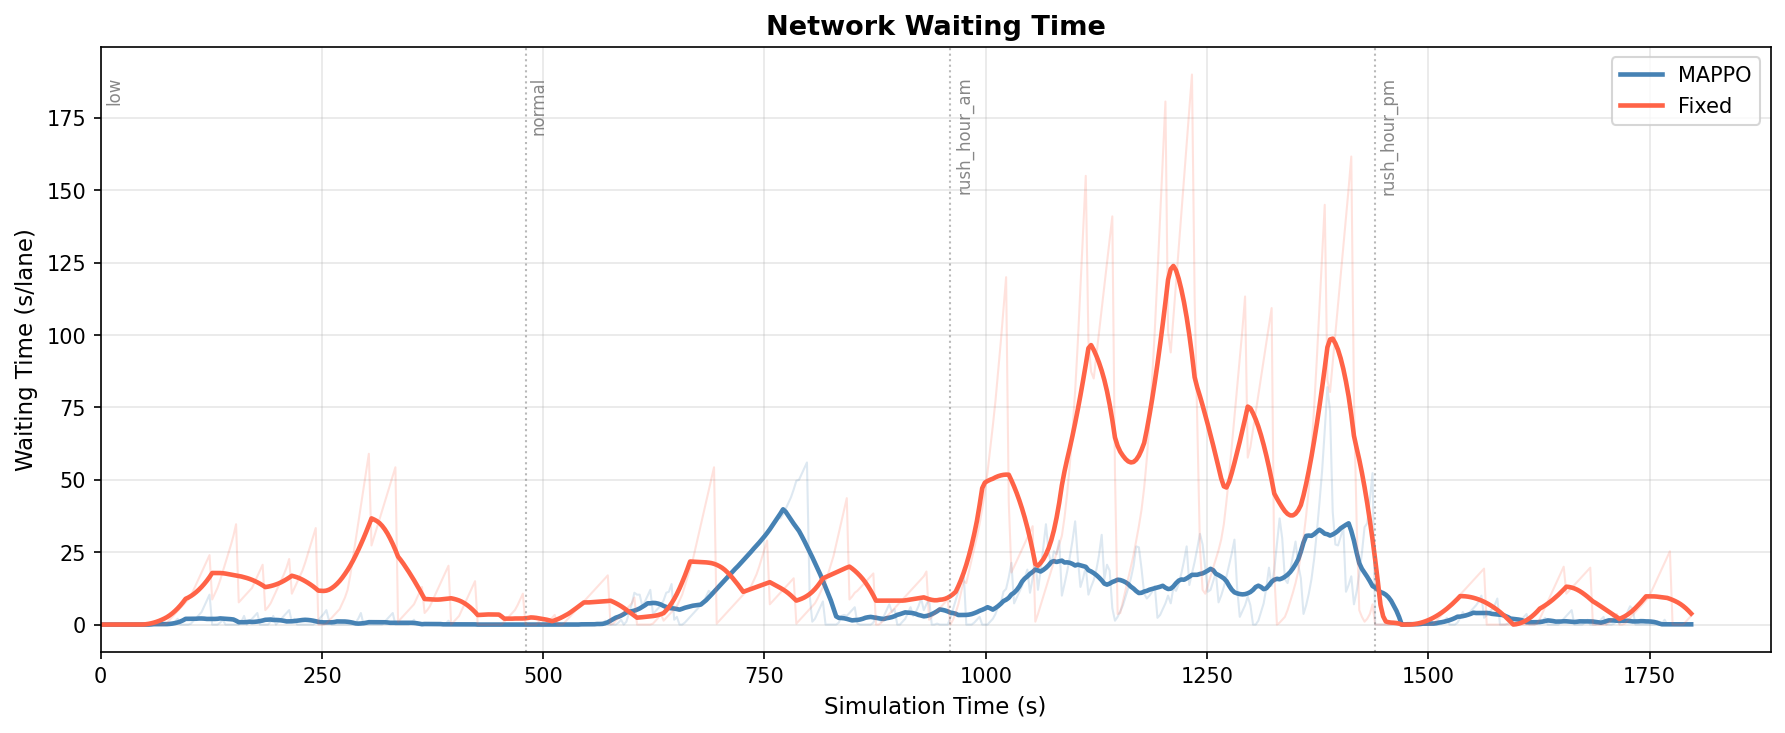
\includegraphics[width=\textwidth]{compare_network_waiting_time.png}}
\caption{Network-wide waiting time per lane over simulation time. MAPPO (blue) vs Fixed-Time (red).}
\label{fig:net_wait}
\end{figure}

\begin{figure}[H]
\centering
\makebox[\textwidth][c]{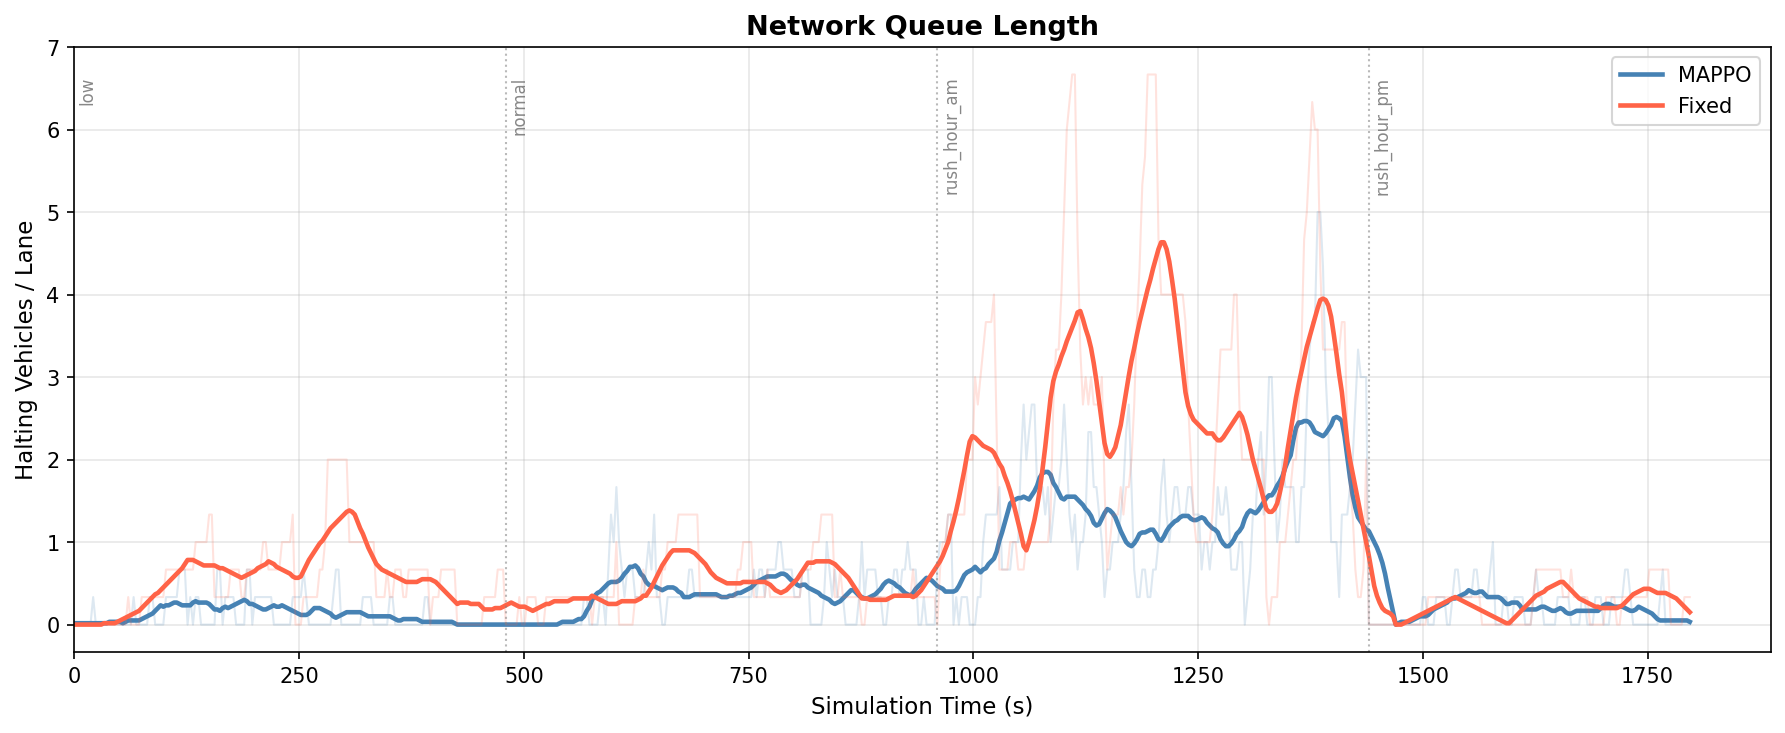
\includegraphics[width=\textwidth]{compare_network_queue_length.png}}
\caption{Network-wide queue length over simulation time.}
\label{fig:net_queue}
\end{figure}

\begin{figure}[H]
\centering
\makebox[\textwidth][c]{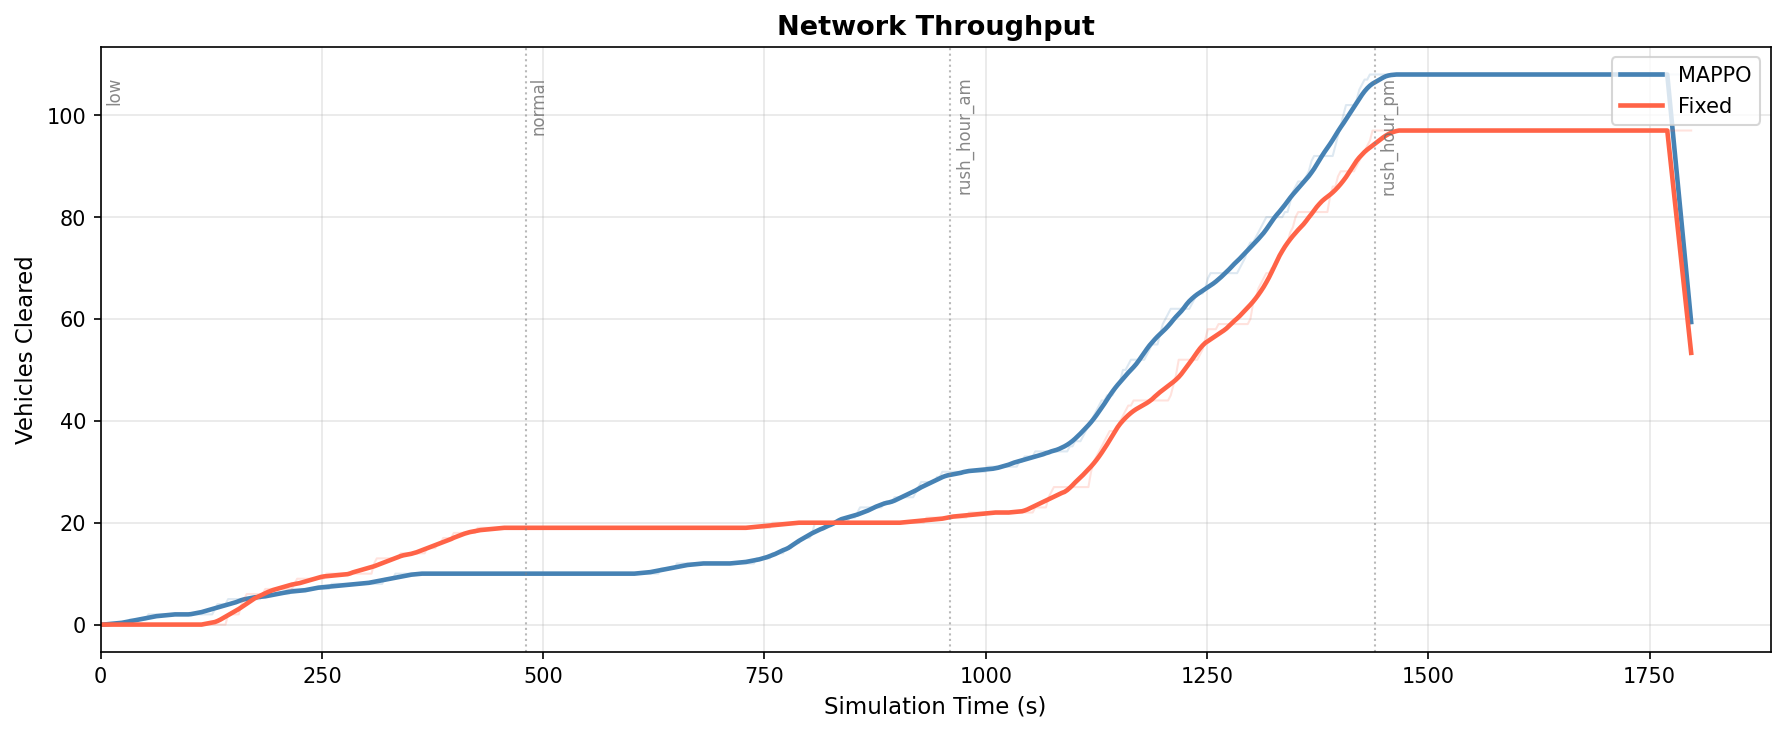
\includegraphics[width=\textwidth]{compare_network_throughput.png}}
\caption{Cumulative network wide throughput over simulation time.}
\label{fig:net_throughput}
\end{figure}

\begin{figure}[H]
\centering
\makebox[\textwidth][c]{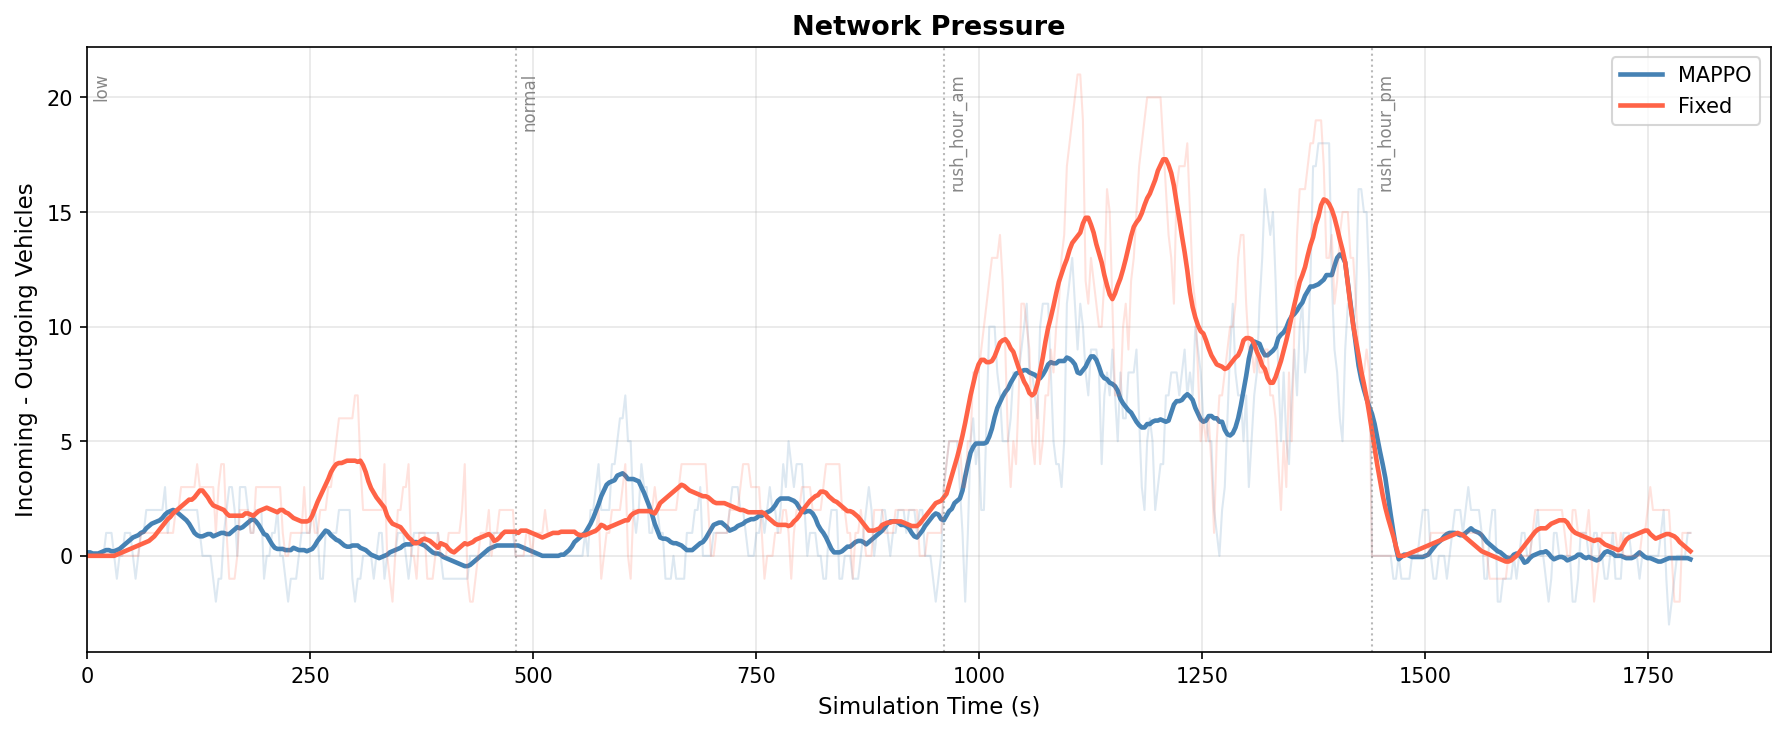
\includegraphics[width=\textwidth]{compare_network_pressure.png}}
\caption{Network-wide traffic pressure over simulation time.}
\label{fig:net_pressure}
\end{figure}

Figure~\ref{fig:net_wait} makes the coordination benefit visible. Fixed-time waiting time climbs steeply into \texttt{rush\_hour\_am}, peaking above 150\,s/lane as queues build across all three junctions simultaneously. MAPPO holds waiting time near zero through the same period, then recovers cleanly when demand drops. The gap is substantial. MAPPO coordinated its response to the demand wave; fixed-time had no mechanism to detect it, let alone adapt.

\subsection{Discussion}

The network wide results answer the core research question. Cooperative multi-agent control reduces congestion across the three-junction A1 corridor in conditions where fixed time control fails. The improvement is largest under the highest-demand scenarios, which are also the scenarios that matter most operationally. The \texttt{rush\_hour\_pm} waiting time result is the one anomaly, explained by the same trade-off from Phase 1. MAPPO's cooperative reward pulls agents toward network throughput rather than per-lane waiting time, so a small wait increase on one approach is rational if it keeps the whole corridor moving.

The fixed-time controller's failure under \texttt{rush\_hour\_am} and \texttt{holiday} is a structural limitation. A fixed cycle has no mechanism to redistribute green time when demand concentrates on specific approaches. MAPPO detects queue build-up through its observation vector and adjusts in real time. The benefit grows with demand intensity because that is exactly when fixed-time's rigid cycle is most costly.

\chapter{Conclusion}

This project set out to address chronic congestion at Palapye's A1 corridor intersections by replacing static signal timing with an adaptive, learning based controller. The work progressed through two phases of increasing scope and complexity, culminating in a cooperative multi-agent system evaluated across six realistic demand scenarios on a corridor network derived from actual Palapye road geometry.

\paragraph{Phase 1: Single-Agent PPO Baseline}
A single PPO agent was trained to control one isolated intersection in SUMO, establishing the project baseline. The evaluation covered 9,000 simulation timesteps across five demand phases (light, moderate, heavy, peak, and extended), comparing the PPO controller against a fixed time controller under identical network conditions, route files, and random seeds. The PPO controller achieved a 48.5\% improvement in throughput ($p < 0.001$), a 27.8\% reduction in queue length ($p < 0.001$), and a 27.3\% reduction in traffic pressure ($p < 0.001$). Aggregate delay was 10.1\% worse overall, although phase-specific analysis showed delays 50--68\% lower during the heavy and peak demand periods. This confirmed that a reinforcement learning controller can learn demand-responsive phase allocation from scratch in simulation and set the benchmark that Phase 2 was designed to surpass at network scale.

A YOLOv8-based vehicle detection and queue estimation module was also developed and validated on sample Palapye traffic footage, showing that camera based sensing could support real world deployment.

\paragraph{Phase 2: MAPPO Multi-Intersection Extension}

The system was extended to all three signalised intersections along the A1 Palapye corridor. Multi-Agent PPO with a Centralised Critic (MAPPO) was implemented under a Centralised Training, Decentralised Execution architecture. A shared Actor network, trained jointly on experience from all three agents, learns to coordinate phase timing across the network rather than optimising each junction in isolation. A cooperative reward signal, green wave pre-computation, and a three stage curriculum over six demand scenarios were added to support learning in the more complex multi-intersection environment.

The MAPPO system was trained over 1.5 million environment steps across six demand scenarios (low, normal, rush\_hour\_am, rush\_hour\_pm, holiday, incident) using a three-stage curriculum. Evaluation was conducted per scenario over 500 simulation timesteps per episode with a single training seed. The MAPPO system produces behaviours not present in the single-agent baseline: cross-junction awareness, anticipatory discharge before downstream pressure builds, and coordination patterns resembling green wave progression during rush-hour conditions. During high demand scenarios, MAPPO reduces mean waiting time by approximately 60\% relative to fixed time control and achieves over 50\% reduction in queue lengths, improvements that the single-intersection PPO baseline, by definition, could not extend to a three-junction corridor.

Together, the two phases validate a clear technical progression: Phase 1 proved that reinforcement learning can learn adaptive signal control at a single junction; Phase 2 demonstrated that cooperative multi-agent learning can extend that capability to a realistic arterial corridor, delivering measurably stronger performance where single-agent and fixed time approaches fail. This contribution, representing one of the first reported applications of cooperative MARL to a signalised corridor in Botswana, establishes a reproducible research platform and quantitative benchmarks on which future work can build.

The findings presented in this report are entirely simulation based. All training and evaluation were conducted within SUMO using synthetically parameterised demand scenarios; no real traffic count data was used for calibration. The results require field validation and calibration against actual turning movements and flow rates before they can be applied to real world signal control. The simulation environment provides a controlled, reproducible basis for algorithmic comparison, but transfer to a live deployment environment will require hardware integration, camera calibration, and regulatory approval.

\chapter{Recommendations}

The MAPPO system represents a substantial upgrade over the single-intersection PPO baseline, but several directions would strengthen it further before any real world deployment.

\textbf{Field traffic count collection.}  The simulation network is synthetically
  parameterised. Real turning movement counts and flow rates, obtained from the
  Botswana Department of Roads or through a manual survey at the three A1
  junctions, would allow the SUMO model to be calibrated to actual demand. This
  would make comparative results against fixed time control more credible and
  allow proper validation of the learned policies.

\textbf{Camera calibration and real time YOLO integration.}  The YOLOv8 module developed
  in Phase 1 should be deployed at one of the A1 junctions with a calibrated
  camera, validated against manual vehicle counts, and integrated into the MAPPO
  observation pipeline. A validation table comparing manual counts to
  YOLO-estimated queue lengths, including detection accuracy, false positive and
  negative rates, and FPS, should be produced before full closed loop integration.

\textbf{Actuated baseline comparison.}The current evaluation compares MAPPO against a
  fixed time controller and a random policy. Adding a vehicle-actuated baseline,
  such as a gap based or Webster optimised controller, would provide a more
  rigorous comparison point.

\textbf{Safety constraints and pedestrian phases.} The current action space does not include dedicated pedestrian crossing phases. A deployment-ready controller must incorporate pedestrian demand signals, minimum green guarantees for pedestrian crossings, and inter-green clearance intervals that meet Botswana road safety standards.

\textbf{Emergency vehicle priority.} The reward function and phase constraints should include a pre emption mechanism that clears priority lanes upon detection of emergency vehicles. This is a standard requirement for any signalised intersection controller considered for real deployment.

\textbf{Enriched observation space.} The current 22-dimensional observation treats all lane vehicles uniformly. Separating turn movement counts from through movement counts would give each agent more precise information for protected-turn phase decisions. Including downstream occupancy from adjacent junctions directly in the local observation, rather than relying solely on the global critic, could also improve decentralised performance at deployment.


\textbf{Extended training with GPU acceleration.}  The current 1.5 million-step training budget is practical for CPU execution but
  conservative. Training for 5-10 million steps with GPU acceleration would let
  the curriculum cover rare edge cases, such as the incident scenario, more
  thoroughly, and allow multi-seed evaluation to quantify result variance.



\appendix

\chapter{PPO Training Script}

\begin{lstlisting}[language=Python, caption={PPO Training Script, Tsotlhe N. Seiphepi (ID: 21001137)}]
"""
Author: Tsotlhe Nayang Seiphepi
Student ID: 21001137

PPO Traffic Signal Control Training Script
This script trains a Proximal Policy Optimization (PPO) agent
within a SUMO based traffic signal control environment.
"""

import os
import time
import torch
from stable_baselines3 import PPO
from stable_baselines3.common.vec_env import DummyVecEnv
from stable_baselines3.common.callbacks import (
    CheckpointCallback, EvalCallback
)
from stable_baselines3.common.monitor import Monitor
from env import SumoEnv


def main():
    """
    Main training entry point for the PPO agent.
    Sets up the environment, logging directories, callbacks,
    hyperparameters, and initiates training.
    """

    # --------------------------------------------------------
    # ENVIRONMENT SETUP
    # --------------------------------------------------------
    sumo_config = "map.sumocfg"

    def make_env():
        """Factory method to create a monitored SUMO environment."""
        return Monitor(SumoEnv(sumo_cfg=sumo_config, use_gui=False))

    # Create vectorized environment
    env = DummyVecEnv([make_env])

    # --------------------------------------------------------
    # LOGGING & DIRECTORY SETUP
    # --------------------------------------------------------
    run_name = time.strftime("PPO_run_%Y%m%d_%H%M%S")
    log_dir = f"./tb_logs/{run_name}/"
    os.makedirs(log_dir, exist_ok=True)

    checkpoint_dir = "./checkpoints/"
    os.makedirs(checkpoint_dir, exist_ok=True)

    # --------------------------------------------------------
    # DEVICE SELECTION
    # --------------------------------------------------------
    device = "cuda" if torch.cuda.is_available() else "cpu"
    print(f"\nUsing device: {device}\n")

    # --------------------------------------------------------
    # CHECKPOINT CALLBACK
    # --------------------------------------------------------
    checkpoint_callback = CheckpointCallback(
        save_freq=5000,
        save_path=checkpoint_dir,
        name_prefix="ppo_traffic"
    )

    # --------------------------------------------------------
    # EVALUATION CALLBACK
    # --------------------------------------------------------
    eval_env = DummyVecEnv([make_env])
    eval_callback = EvalCallback(
        eval_env,
        best_model_save_path="./best_model/",
        log_path="./eval_logs/",
        eval_freq=4000,
        deterministic=True,
        render=False
    )

    # --------------------------------------------------------
    # PPO MODEL INITIALISATION
    # --------------------------------------------------------
    model = PPO(
        policy="MlpPolicy",
        env=env,
        verbose=1,
        tensorboard_log=log_dir,
        device=device,
        learning_rate=3e-4,
        n_steps=1024,
        batch_size=64,
        n_epochs=5,
        gamma=0.99,
        gae_lambda=0.95,
        clip_range=0.2
    )

    # --------------------------------------------------------
    # TRAINING
    # --------------------------------------------------------
    TOTAL_TIMESTEPS = 8000

    print(f"Training PPO Agent for {TOTAL_TIMESTEPS} timesteps...")
    model.learn(
        total_timesteps=TOTAL_TIMESTEPS,
        callback=[checkpoint_callback, eval_callback],
        tb_log_name="PPO_traffic_signal"
    )

    # --------------------------------------------------------
    # SAVE FINAL MODEL
    # --------------------------------------------------------
    model.save("ppo_traffic_final")

    print("\nTraining completed successfully!")
    print("Final model saved as: ppo_traffic_final.zip")
    print(f"TensorBoard logs saved in: {log_dir}")


if __name__ == "__main__":
    main()
\end{lstlisting}


\begin{lstlisting}[language=Python, caption={PPO Testing Script, Tsotlhe N. Seiphepi (ID: 21001137)}]
import os
import time
import torch
from stable_baselines3 import PPO
from stable_baselines3.common.vec_env import DummyVecEnv
from stable_baselines3.common.callbacks import CheckpointCallback, EvalCallback
from stable_baselines3.common.monitor import Monitor
from env import SumoEnv


def main():

    # ============================================================
    # ENVIRONMENT SETUP
    # ============================================================
    sumo_config = "map.sumocfg"

    def make_env():
        return Monitor(SumoEnv(sumo_cfg=sumo_config, use_gui=False))

    env = DummyVecEnv([make_env])

    # ============================================================
    # LOGGING + FOLDERS
    # ============================================================
    run_name = time.strftime("PPO_run_%Y%m%d_%H%M%S")
    log_dir = f"./tb_logs/{run_name}/"
    os.makedirs(log_dir, exist_ok=True)

    checkpoint_dir = "./checkpoints/"
    os.makedirs(checkpoint_dir, exist_ok=True)

    # ============================================================
    # DEVICE SELECTION
    # ============================================================
    device = "cuda" if torch.cuda.is_available() else "cpu"
    print(f"\nUsing device: {device}\n")

    # ============================================================
    # CHECKPOINT CALLBACK
    # ============================================================
    checkpoint_callback = CheckpointCallback(
        save_freq=5000,   # save more frequently since 8000 steps is small
        save_path=checkpoint_dir,
        name_prefix="ppo_traffic"
    )

    # ============================================================
    # EVAL CALLBACK
    # ============================================================
    eval_env = DummyVecEnv([make_env])
    eval_callback = EvalCallback(
        eval_env,
        best_model_save_path="./best_model/",
        log_path="./eval_logs/",
        eval_freq=4000,
        deterministic=True,
        render=False
    )

    # ============================================================
    # PPO MODEL
    # ============================================================
    model = PPO(
        policy="MlpPolicy",
        env=env,
        verbose=1,
        tensorboard_log=log_dir,
        device=device,
        learning_rate=3e-4,
        n_steps=1024,
        batch_size=64,
        n_epochs=5,
        gamma=0.99,
        gae_lambda=0.95,
        clip_range=0.2
    )

    # ============================================================
    # TRAINING
    # ============================================================
    TOTAL_TIMESTEPS = 8000

    print(f"�� Training PPO Agent for {TOTAL_TIMESTEPS} timesteps...")
    model.learn(
        total_timesteps=TOTAL_TIMESTEPS,
        callback=[checkpoint_callback, eval_callback],
        tb_log_name="PPO_traffic_signal"
    )

    # ============================================================
    # SAVE FINAL MODEL
    # ============================================================
    model.save("ppo_traffic_final")

    print("\n�� Training completed successfully!")
    print("Final model saved as: ppo_traffic_final.zip")
    print(f"TensorBoard logs saved in: {log_dir}")


if __name__ == "__main__":
    main()

\end{lstlisting}
\begin{lstlisting}
\end{lstlisting}


\begin{lstlisting}
\end{lstlisting}



\begin{lstlisting}
\end{lstlisting}





\begin{lstlisting}[language=XML, caption={SUMO Palapye Location Code, Tsotlhe N. Seiphepi (ID: 21001137)}]
<?xml version="1.0" encoding="UTF-8"?>

<!-- generated on 2025-11-18 11:38:53 by Eclipse SUMO netedit Version 1.24.0
<neteditConfiguration xmlns:qxsi="http://www.w3.org/2001/XMLSchema-instance" xsi:noNamespaceSchemaLocation="http://sumo.dlr.de/xsd/neteditConfiguration.xsd">

    <input>
        <sumocfg-file value="map.sumocfg"/>
        <additional-files value="C:/Users/tsotl/DRL TRAFFIC OPTIMIZATION - Copy/vtypes.add.xml, C:/Users/tsotl/DRL TRAFFIC OPTIMIZATION - Copy/tls.add.xml"/>
        <sumo-net-file value="C:/Users/tsotl/DRL TRAFFIC OPTIMIZATION - Copy/lol.xml"/>
    </input>

    <output>
        <output-file value="C:/Users/tsotl/DRL TRAFFIC OPTIMIZATION - Copy/lol.xml"/>
    </output>

    <processing>
        <geometry.min-radius.fix.railways value="false"/>
        <geometry.avoid-overlap value="false"/>
        <geometry.max-grade.fix value="false"/>
        <offset.disable-normalization value="true"/>
        <lefthand value="1"/>
    </processing>

    <junctions>
        <no-turnarounds value="true"/>
        <junctions.corner-detail value="5"/>
        <junctions.limit-turn-speed value="5.50"/>
        <rectangular-lane-cut value="0"/>
    </junctions>

    <pedestrian>
        <walkingareas value="0"/>
    </pedestrian>

    <netedit>
        <ignore.routeelements value="false"/>
    </netedit>

</neteditConfiguration>
-->

<net version="1.20" junctionCornerDetail="5" lefthand="true" limitTurnSpeed="5.50" avoidOverlap="0" xmlns:xsi="http://www.w3.org/2001/XMLSchema-instance" xsi:noNamespaceSchemaLocation="http://sumo.dlr.de/xsd/net_file.xsd">

    <location netOffset="0.00,0.00" convBoundary="508842.46,-2492852.72,510825.89,-2492017.05" origBoundary="27.085993,-22.542254,27.105286,-22.534714" projParameter="+proj=utm +zone=35 +ellps=WGS84 +datum=WGS84 +units=m +no_defs"/>

    <type id="highway.residential" priority="3" numLanes="1" speed="13.89" disallow="tram rail_urban rail rail_electric rail_fast ship container cable_car subway aircraft wheelchair scooter drone" oneway="0"/>
    <type id="highway.trunk" priority="13" numLanes="2" speed="27.78" disallow="pedestrian bicycle tram rail_urban rail rail_electric rail_fast ship container cable_car subway aircraft wheelchair scooter drone" oneway="0"/>
    <type id="highway.unclassified" priority="4" numLanes="1" speed="13.89" disallow="tram rail_urban rail rail_electric rail_fast ship container cable_car subway aircraft wheelchair scooter drone" oneway="0"/>

    <edge id=":4557655746_0" function="internal">
        <lane id=":4557655746_0_0" index="0" disallow="pedestrian bicycle tram rail_urban rail rail_electric rail_fast ship container cable_car subway aircraft wheelchair scooter drone" speed="15.28" length="6.74" shape="509136.07,-2492440.65 509135.48,-2492442.56 509135.02,-2492443.85 509134.47,-2492445.10 509133.58,-2492446.89"/>
        <lane id=":4557655746_0_1" index="1" disallow="pedestrian bicycle tram rail_urban rail rail_electric rail_fast ship container cable_car subway aircraft wheelchair scooter drone" speed="15.28" length="7.43" shape="509133.01,-2492439.72 509132.88,-2492441.84 509133.50,-2492443.39 509134.02,-2492444.90 509133.58,-2492446.89"/>
    </edge>
    <edge id=":4557655751_0" function="internal">
        <lane id=":4557655751_0_0" index="0" disallow="pedestrian bicycle tram rail_urban rail rail_electric rail_fast ship container cable_car subway aircraft wheelchair scooter drone" speed="16.67" length="12.53" shape="509143.05,-2492419.28 509138.97,-2492431.07"/>
        <lane id=":4557655751_0_1" index="1" disallow="pedestrian bicycle tram rail_urban rail rail_electric rail_fast ship container cable_car subway aircraft wheelchair scooter drone" speed="16.67" length="12.53" shape="509140.02,-2492418.26 509135.91,-2492430.15"/>
    </edge>
    <edge id=":4557655751_2" function="internal">
        <lane id=":4557655751_2_0" index="0" disallow="pedestrian bicycle tram rail_urban rail rail_electric rail_fast ship container cable_car subway aircraft wheelchair scooter drone" speed="10.37" length="12.50" shape="509129.76,-2492428.28 509130.88,-2492425.00 509131.26,-2492421.90 509130.89,-2492418.98 509129.77,-2492416.24"/>
    </edge>
    <edge id=":4557655751_3" function="internal">
        <lane id=":4557655751_3_0" index="0" disallow="pedestrian bicycle tram rail_urban rail rail_electric rail_fast ship container cable_car subway aircraft wheelchair scooter drone" speed="16.67" length="12.74" shape="509129.76,-2492428.28 509131.22,-2492424.78 509132.07,-2492422.33 509132.81,-2492419.83 509133.96,-2492416.21"/>
        <lane id=":4557655751_3_1" index="1" disallow="pedestrian bicycle tram rail_urban rail rail_electric rail_fast ship container cable_car subway aircraft wheelchair scooter drone" speed="16.67" length="12.74" shape="509132.85,-2492429.22 509134.29,-2492425.75 509135.12,-2492423.30 509135.85,-2492420.83 509136.99,-2492417.23"/>
    </edge>
    <edge id=":4557655752_0" function="internal">
        <lane id=":4557655752_0_0" index="0" disallow="pedestrian bicycle tram rail_urban rail rail_electric rail_fast ship container cable_car subway aircraft wheelchair scooter drone" speed="15.28" length="8.26" shape="509123.40,-2492443.52 509124.41,-2492441.36 509124.95,-2492439.82 509125.45,-2492438.25 509126.34,-2492436.03"/>
        <lane id=":4557655752_0_1" index="1" disallow="pedestrian bicycle tram rail_urban rail rail_electric rail_fast ship container cable_car subway aircraft wheelchair scooter drone" speed="15.28" length="8.26" shape="509123.40,-2492443.52 509124.88,-2492441.56 509126.38,-2492440.56 509127.83,-2492439.54 509129.18,-2492437.52"/>
    </edge>
    <edge id=":6073919354_0" function="internal">
        <lane id=":6073919354_0_0" index="0" disallow="pedestrian bicycle tram rail_urban rail rail_electric rail_fast ship container cable_car subway aircraft wheelchair scooter drone" speed="7.53" length="12.36" shape="509156.08,-2492409.80 509152.10,-2492408.87 509148.99,-2492409.00 509146.75,-2492410.19 509145.37,-2492412.43"/>
    </edge>
    <edge id=":6073919354_1" function="internal">
        <lane id=":6073919354_1_0" index="0" disallow="tram rail_urban rail rail_electric rail_fast ship container cable_car subway aircraft wheelchair scooter drone" speed="13.89" length="24.55" shape="509156.08,-2492409.80 509132.69,-2492402.36"/>
    </edge>
    <edge id=":6073919354_2" function="internal">
        <lane id=":6073919354_2_0" index="0" disallow="pedestrian bicycle tram rail_urban rail rail_electric rail_fast ship container cable_car subway aircraft wheelchair scooter drone" speed="9.23" length="7.17" shape="509156.08,-2492409.80 509149.74,-2492407.07 509149.53,-2492406.89"/>
    </edge>
    <edge id=":6073919354_10" function="internal">
        <lane id=":6073919354_10_0" index="0" disallow="pedestrian bicycle tram rail_urban rail rail_electric rail_fast ship container cable_car subway aircraft wheelchair scooter drone" speed="9.23" length="13.32" shape="509149.53,-2492406.89 509145.78,-2492403.81 509144.17,-2492400.04 509144.94,-2492395.74"/>
    </edge>
    <edge id=":6073919354_3" function="internal">
        <lane id=":6073919354_3_0" index="0" disallow="pedestrian bicycle tram rail_urban rail rail_electric rail_fast ship container cable_car subway aircraft wheelchair scooter drone" speed="6.44" length="9.11" shape="509153.66,-2492399.47 509153.13,-2492401.95 509153.53,-2492403.96 509154.85,-2492405.51 509157.09,-2492406.59"/>
    </edge>
    <edge id=":6073919354_4" function="internal">
        <lane id=":6073919354_4_0" index="0" disallow="pedestrian bicycle tram rail_urban rail rail_electric rail_fast ship container cable_car subway aircraft wheelchair scooter drone" speed="16.67" length="15.75" shape="509150.71,-2492398.21 509148.63,-2492402.33 509146.46,-2492404.78 509144.33,-2492407.25 509142.34,-2492411.40"/>
    </edge>
    <edge id=":6073919354_5" function="internal">
        <lane id=":6073919354_5_0" index="0" disallow="pedestrian bicycle tram rail_urban rail rail_electric rail_fast ship container cable_car subway aircraft wheelchair scooter drone" speed="9.12" length="6.29" shape="509147.76,-2492396.95 509145.59,-2492400.66 509143.93,-2492401.76"/>
    </edge>
    <edge id=":6073919354_11" function="internal">
        <lane id=":6073919354_11_0" index="0" disallow="pedestrian bicycle tram rail_urban rail rail_electric rail_fast ship container cable_car subway aircraft wheelchair scooter drone" speed="9.12" length="11.69" shape="509143.93,-2492401.76 509142.36,-2492402.80 509138.05,-2492403.36 509132.69,-2492402.36"/>
    </edge>
    <edge id=":6073919354_6" function="internal">
        <lane id=":6073919354_6_0" index="0" disallow="tram rail_urban rail rail_electric rail_fast ship container cable_car subway aircraft wheelchair scooter drone" speed="13.89" length="24.58" shape="509133.62,-2492399.29 509157.09,-2492406.59"/>
    </edge>
    <edge id=":6073919354_7" function="internal">
        <lane id=":6073919354_7_0" index="0" disallow="pedestrian bicycle tram rail_urban rail rail_electric rail_fast ship container cable_car subway aircraft wheelchair scooter drone" speed="8.62" length="5.73" shape="509133.62,-2492399.29 509138.52,-2492401.38 509138.83,-2492401.64"/>
    </edge>
    <edge id=":6073919354_12" function="internal">
        <lane id=":6073919354_12_0" index="0" disallow="pedestrian bicycle tram rail_urban rail rail_electric rail_fast ship container cable_car subway aircraft wheelchair scooter drone" speed="8.62" length="11.29" shape="509138.83,-2492401.64 509141.61,-2492404.09 509142.89,-2492407.43 509142.34,-2492411.40"/>
    </edge>
    <edge id=":6073919354_8" function="internal">
        <lane id=":6073919354_8_0" index="0" disallow="pedestrian bicycle tram rail_urban rail rail_electric rail_fast ship container cable_car subway aircraft wheelchair scooter drone" speed="16.67" length="16.23" shape="509136.28,-2492409.35 509138.45,-2492404.65 509140.84,-2492401.40 509143.12,-2492398.73 509144.94,-2492395.74"/>
    </edge>
    <edge id=":6073919354_9" function="internal">
        <lane id=":6073919354_9_0" index="0" disallow="pedestrian bicycle tram rail_urban rail rail_electric rail_fast ship container cable_car subway aircraft wheelchair scooter drone" speed="9.53" length="4.06" shape="509139.31,-2492410.38 509141.50,-2492406.96"/>
    </edge>
    <edge id=":6073919354_13" function="internal">
        <lane id=":6073919354_13_0" index="0" disallow="pedestrian bicycle tram rail_urban rail rail_electric rail_fast ship container cable_car subway aircraft wheelchair scooter drone" speed="9.53" length="16.17" shape="509141.50,-2492406.96 509145.19,-2492405.18 509150.39,-2492405.06 509157.09,-2492406.59"/>
    </edge>
    <edge id=":6145489304_0" function="internal">
        <lane id=":6145489304_0_0" index="0" disallow="pedestrian bicycle tram rail_urban rail rail_electric rail_fast ship container cable_car subway aircraft wheelchair scooter drone" speed="16.67" length="26.96" shape="509168.94,-2492342.39 509167.67,-2492347.15 509166.33,-2492353.76 509164.66,-2492361.24 509162.38,-2492368.63"/>
        <lane id=":6145489304_0_1" index="1" disallow="pedestrian bicycle tram rail_urban rail rail_electric rail_fast ship container cable_car subway aircraft wheelchair scooter drone" speed="16.67" length="26.96" shape="509168.94,-2492342.39 509159.39,-2492367.49"/>
    </edge>
    <edge id=":6145489304_2" function="internal">
        <lane id=":6145489304_2_0" index="0" disallow="pedestrian bicycle tram rail_urban rail rail_electric rail_fast ship container cable_car subway aircraft wheelchair scooter drone" speed="15.28" length="26.74" shape="509152.86,-2492364.63 509155.78,-2492359.85 509159.78,-2492353.16 509163.61,-2492346.38 509165.99,-2492341.35"/>
    </edge>
    <edge id=":6145489304_3" function="internal">
        <lane id=":6145489304_3_0" index="0" disallow="pedestrian bicycle tram rail_urban rail rail_electric rail_fast ship container cable_car subway aircraft wheelchair scooter drone" speed="16.67" length="26.78" shape="509156.38,-2492366.35 509165.99,-2492341.35"/>
    </edge>
    <edge id=":6145489310_0" function="internal">
        <lane id=":6145489310_0_0" index="0" disallow="tram rail_urban rail rail_electric rail_fast ship container cable_car subway aircraft wheelchair scooter drone" speed="13.89" length="9.85" shape="509121.01,-2492402.67 509118.97,-2492400.55 509117.61,-2492399.00 509116.06,-2492397.77 509113.45,-2492396.60"/>
    </edge>
    <edge id=":6145489310_1" function="internal">
        <lane id=":6145489310_1_0" index="0" disallow="tram rail_urban rail rail_electric rail_fast ship container cable_car subway aircraft wheelchair scooter drone" speed="13.89" length="12.06" shape="509125.01,-2492400.02 509113.45,-2492396.60"/>
    </edge>
    <edge id=":6145489310_2" function="internal">
        <lane id=":6145489310_2_0" index="0" disallow="tram rail_urban rail rail_electric rail_fast ship container cable_car subway aircraft wheelchair scooter drone" speed="13.89" length="12.07" shape="509114.52,-2492393.58 509117.67,-2492394.37 509120.37,-2492394.38 509123.10,-2492393.85 509126.33,-2492393.00"/>
    </edge>
    <edge id=":6145489310_3" function="internal">
        <lane id=":6145489310_3_0" index="0" disallow="tram rail_urban rail rail_electric rail_fast ship container cable_car subway aircraft wheelchair scooter drone" speed="13.89" length="11.91" shape="509114.52,-2492393.58 509125.94,-2492396.96"/>
    </edge>
    <edge id=":J1_0" function="internal">
        <lane id=":J1_0_0" index="0" disallow="pedestrian bicycle tram rail_urban rail rail_electric rail_fast ship container cable_car subway aircraft wheelchair scooter drone" speed="16.67" length="8.82" shape="509157.34,-2492381.87 509156.79,-2492384.48 509157.04,-2492386.39 509157.29,-2492388.30 509156.77,-2492390.92"/>
        <lane id=":J1_0_1" index="1" disallow="pedestrian bicycle tram rail_urban rail rail_electric rail_fast ship container cable_car subway aircraft wheelchair scooter drone" speed="16.67" length="8.82" shape="509157.34,-2492381.87 509153.78,-2492389.77"/>
        <lane id=":J1_0_2" index="2" disallow="pedestrian bicycle tram rail_urban rail rail_electric rail_fast ship container cable_car subway aircraft wheelchair scooter drone" speed="16.67" length="8.82" shape="509154.33,-2492380.78 509150.80,-2492388.62"/>
    </edge>

    <edge id="-465932558#0" from="6073919354" to="4557655751" priority="13" type="highway.trunk" shape="509143.20,-2492403.88 509139.71,-2492414.19 509134.26,-2492430.31">
        <lane id="-465932558#0_0" index="0" disallow="pedestrian bicycle tram rail_urban rail rail_electric rail_fast ship container cable_car subway aircraft wheelchair scooter drone" speed="16.67" length="7.24" shape="509145.37,-2492412.43 509144.26,-2492415.73 509143.05,-2492419.28"/>
        <lane id="-465932558#0_1" index="1" disallow="pedestrian bicycle tram rail_urban rail rail_electric rail_fast ship container cable_car subway aircraft wheelchair scooter drone" speed="16.67" length="7.24" shape="509142.34,-2492411.40 509141.23,-2492414.70 509140.02,-2492418.26"/>
        <param key="ref" value="A1"/>
    </edge>
    <edge id="-465932558#1" from="6145489304" to="J1" priority="13" type="highway.trunk" shape="509168.64,-2492338.65 509152.90,-2492380.06 509148.10,-2492391.35">
        <lane id="-465932558#1_0" index="0" disallow="pedestrian bicycle tram rail_urban rail rail_electric rail_fast ship container cable_car subway aircraft wheelchair scooter drone" speed="16.67" length="14.20" shape="509162.38,-2492368.63 509157.34,-2492381.87"/>
        <lane id="-465932558#1_1" index="1" disallow="pedestrian bicycle tram rail_urban rail rail_electric rail_fast ship container cable_car subway aircraft wheelchair scooter drone" speed="16.67" length="14.20" shape="509159.39,-2492367.49 509154.38,-2492380.66 509154.33,-2492380.78"/>
        <param key="ref" value="A1"/>
    </edge>
    <edge id="-465932558#1.34" from="J1" to="6073919354" priority="13" type="highway.trunk">
        <lane id="-465932558#1.34_0" index="0" disallow="pedestrian bicycle tram rail_urban rail rail_electric rail_fast ship container cable_car subway aircraft wheelchair scooter drone" speed="16.67" length="8.98" shape="509156.77,-2492390.92 509153.66,-2492399.47"/>
        <lane id="-465932558#1.34_1" index="1" disallow="pedestrian bicycle tram rail_urban rail rail_electric rail_fast ship container cable_car subway aircraft wheelchair scooter drone" speed="16.67" length="8.98" shape="509153.78,-2492389.77 509150.71,-2492398.21"/>
        <lane id="-465932558#1.34_2" index="2" disallow="pedestrian bicycle tram rail_urban rail rail_electric rail_fast ship container cable_car subway aircraft wheelchair scooter drone" speed="16.67" length="8.98" shape="509150.80,-2492388.62 509147.76,-2492396.95"/>
        <param key="ref" value="A1"/>
    </edge>
    <edge id="-465932558#2" from="6073363232" to="6145489304" priority="13" type="highway.trunk" shape="509271.33,-2492017.05 509264.16,-2492040.35 509258.95,-2492064.87 509252.03,-2492097.42 509246.66,-2492125.37 509225.73,-2492177.46 509198.28,-2492254.57 509179.33,-2492305.02 509172.02,-2492329.68 509168.64,-2492338.65">
        <lane id="-465932558#2_0" index="0" disallow="pedestrian bicycle tram rail_urban rail rail_electric rail_fast ship container cable_car subway aircraft wheelchair scooter drone" speed="16.67" length="341.86" shape="509272.86,-2492017.52 509265.71,-2492040.75 509260.52,-2492065.20 509253.60,-2492097.74 509248.20,-2492125.82 509227.23,-2492178.03 509199.78,-2492255.12 509180.85,-2492305.53 509173.54,-2492330.19 509168.94,-2492342.39"/>
        <param key="ref" value="A1"/>
    </edge>
    <edge id="-470773638#0" from="6145489310" to="4649671177" priority="4" type="highway.unclassified" shape="509112.24,-2492394.47 509026.62,-2492363.96 509007.89,-2492357.19 508972.70,-2492346.11 508933.69,-2492339.09 508889.60,-2492331.96 508871.14,-2492328.97 508842.46,-2492325.40">
        <lane id="-470773638#0_0" index="0" disallow="tram rail_urban rail rail_electric rail_fast ship container cable_car subway aircraft wheelchair scooter drone" speed="13.89" length="281.10" shape="509113.45,-2492396.60 509026.08,-2492365.47 509007.38,-2492358.71 508972.32,-2492347.67 508933.42,-2492340.67 508889.34,-2492333.54 508870.91,-2492330.55 508842.26,-2492326.99"/>
    </edge>
    <edge id="-470773638#1" from="6073919354" to="6145489310" priority="4" type="highway.unclassified" shape="509143.20,-2492403.88 509112.24,-2492394.47">
        <lane id="-470773638#1_0" index="0" disallow="tram rail_urban rail rail_electric rail_fast ship container cable_car subway aircraft wheelchair scooter drone" speed="13.89" length="8.02" shape="509132.69,-2492402.36 509125.01,-2492400.02"/>
    </edge>
    <edge id="-E5" from="J10" to="6073919354" priority="-1" spreadType="roadCenter" shape="509226.77,-2492431.35 509143.20,-2492403.88">
        <lane id="-E5_0" index="0" speed="13.89" length="73.89" shape="509226.27,-2492432.87 509156.08,-2492409.80"/>
    </edge>
    <edge id="460085149" from="4557655751" to="4557655746" priority="13" type="highway.trunk" spreadType="center" shape="509137.44,-2492430.61 509132.54,-2492448.47 509133.62,-2492443.22">
        <lane id="460085149_0" index="0" disallow="pedestrian bicycle tram rail_urban rail rail_electric rail_fast ship container cable_car subway aircraft wheelchair scooter drone" speed="16.67" length="10.00" shape="509138.97,-2492431.07 509136.07,-2492440.65"/>
        <lane id="460085149_1" index="1" disallow="pedestrian bicycle tram rail_urban rail rail_electric rail_fast ship container cable_car subway aircraft wheelchair scooter drone" speed="16.67" length="10.00" shape="509135.91,-2492430.15 509133.01,-2492439.72"/>
        <param key="ref" value="A1"/>
    </edge>
    <edge id="465932558#0" from="4557655751" to="6073919354" priority="13" type="highway.trunk" spreadType="roadCenter" shape="509134.26,-2492430.31 509143.20,-2492403.88">
        <lane id="465932558#0_0" index="0" disallow="pedestrian bicycle tram rail_urban rail rail_electric rail_fast ship container cable_car subway aircraft wheelchair scooter drone" speed="16.67" length="7.24" shape="509133.96,-2492416.21 509136.28,-2492409.35"/>
        <lane id="465932558#0_1" index="1" disallow="pedestrian bicycle tram rail_urban rail rail_electric rail_fast ship container cable_car subway aircraft wheelchair scooter drone" speed="16.67" length="7.24" shape="509136.99,-2492417.23 509139.31,-2492410.38"/>
        <param key="ref" value="A1"/>
    </edge>
    <edge id="465932558#1" from="6073919354" to="6145489304" priority="13" type="highway.trunk" shape="509143.20,-2492403.88 509148.67,-2492391.08 509168.64,-2492338.65">
        <lane id="465932558#1_0" index="0" disallow="pedestrian bicycle tram rail_urban rail rail_electric rail_fast ship container cable_car subway aircraft wheelchair scooter drone" speed="16.67" length="31.54" shape="509144.94,-2492395.74 509147.19,-2492390.48 509156.38,-2492366.35"/>
        <param key="ref" value="A1"/>
    </edge>
    <edge id="465932558#2" from="6145489304" to="6073363232" priority="13" type="highway.trunk" shape="509168.64,-2492338.65 509171.78,-2492329.72 509179.33,-2492305.02 509198.28,-2492254.57 509225.73,-2492177.46 509246.66,-2492125.37 509252.03,-2492097.42 509258.95,-2492064.87 509264.16,-2492040.35 509271.33,-2492017.05">
        <lane id="465932558#2_0" index="0" disallow="pedestrian bicycle tram rail_urban rail rail_electric rail_fast ship container cable_car subway aircraft wheelchair scooter drone" speed="16.67" length="341.72" shape="509165.99,-2492341.35 509170.26,-2492329.22 509177.81,-2492304.50 509196.78,-2492254.02 509224.23,-2492176.89 509245.12,-2492124.92 509250.46,-2492097.10 509257.38,-2492064.54 509262.61,-2492039.95 509269.80,-2492016.58"/>
        <param key="ref" value="A1"/>
    </edge>
    <edge id="470773638#0" from="4649671177" to="6145489310" priority="4" type="highway.unclassified" shape="508842.46,-2492325.40 508871.14,-2492328.97 508889.60,-2492331.96 508933.69,-2492339.09 508972.70,-2492346.11 509007.89,-2492357.19 509026.62,-2492363.96 509112.24,-2492394.47">
        <lane id="470773638#0_0" index="0" disallow="tram rail_urban rail rail_electric rail_fast ship container cable_car subway aircraft wheelchair scooter drone" speed="13.89" length="281.80" shape="508842.66,-2492323.81 508871.37,-2492327.39 508889.86,-2492330.38 508933.96,-2492337.51 508973.08,-2492344.55 509008.40,-2492355.67 509027.16,-2492362.45 509114.52,-2492393.58"/>
    </edge>
    <edge id="470773638#1" from="6145489310" to="6073919354" priority="4" type="highway.unclassified" shape="509112.24,-2492394.47 509143.20,-2492403.88">
        <lane id="470773638#1_0" index="0" disallow="tram rail_urban rail rail_electric rail_fast ship container cable_car subway aircraft wheelchair scooter drone" speed="13.89" length="8.02" shape="509125.94,-2492396.96 509133.62,-2492399.29"/>
    </edge>
    <edge id="655985522" from="4557655751" to="6145489310" priority="3" type="highway.residential" spreadType="center" shape="509134.26,-2492430.31 509130.33,-2492417.23 509123.42,-2492404.93 509112.24,-2492394.47">
        <lane id="655985522_0" index="0" disallow="tram rail_urban rail rail_electric rail_fast ship container cable_car subway aircraft wheelchair scooter drone" speed="13.89" length="16.28" shape="509129.77,-2492416.24 509123.42,-2492404.93 509121.01,-2492402.67"/>
    </edge>
    <edge id="655985523" from="6145489310" to="6145489304" priority="3" type="highway.residential" spreadType="center" shape="509112.24,-2492394.47 509122.97,-2492393.85 509130.21,-2492392.03 509138.31,-2492388.59 509168.64,-2492338.65">
        <lane id="655985523_0" index="0" disallow="tram rail_urban rail rail_electric rail_fast ship container cable_car subway aircraft wheelchair scooter drone" speed="13.89" length="40.83" shape="509126.33,-2492393.00 509130.21,-2492392.03 509138.31,-2492388.59 509152.86,-2492364.63"/>
    </edge>
    <edge id="682411362" from="4557655752" to="4557655751" priority="13" type="highway.trunk" spreadType="center" shape="509125.92,-2492440.50 509127.12,-2492438.21 509132.84,-2492425.29">
        <lane id="682411362_0" index="0" disallow="pedestrian bicycle tram rail_urban rail rail_electric rail_fast ship container cable_car subway aircraft wheelchair scooter drone" speed="16.67" length="8.77" shape="509126.34,-2492436.03 509129.76,-2492428.28"/>
        <lane id="682411362_1" index="1" disallow="pedestrian bicycle tram rail_urban rail rail_electric rail_fast ship container cable_car subway aircraft wheelchair scooter drone" speed="16.67" length="8.77" shape="509129.18,-2492437.52 509132.85,-2492429.22"/>
        <param key="ref" value="A1"/>
    </edge>
    <edge id="E0" from="J0" to="4557655752" priority="-1">
        <lane id="E0_0" index="0" speed="13.89" length="119.24" shape="509068.35,-2492549.29 509123.40,-2492443.52"/>
    </edge>
    <edge id="E5" from="6073919354" to="J10" priority="-1" spreadType="roadCenter" shape="509143.20,-2492403.88 509165.57,-2492410.95 509226.77,-2492431.35">
        <lane id="E5_0" index="0" speed="13.89" length="73.93" shape="509157.09,-2492406.59 509166.06,-2492409.43 509227.28,-2492429.83"/>
    </edge>
    <edge id="E6" from="4557655746" to="J9" priority="-1">
        <lane id="E6_0" index="0" speed="13.89" length="120.42" shape="509133.58,-2492446.89 509080.01,-2492554.74"/>
    </edge>

    <tlLogic id="6073919354" type="static" programID="0" offset="0">
        <phase duration="36" state="rrrGGgrrGg"/>
        <phase duration="4"  state="rrryygrryg"/>
        <phase duration="6"  state="rrrrrGrrrG"/>
        <phase duration="4"  state="rrrrryrrry"/>
        <phase duration="36" state="GGgrrrGgrr"/>
        <phase duration="4"  state="yyyrrryyrr"/>
    </tlLogic>

    <junction id="1420333935" type="dead_end" x="510825.89" y="-2492852.72" incLanes="" intLanes="" shape="510825.89,-2492852.72"/>
    <junction id="4557655746" type="unregulated" x="509133.62" y="-2492443.22" incLanes="460085149_0 460085149_1" intLanes=":4557655746_0_0 :4557655746_0_1" shape="509132.15,-2492446.18 509135.02,-2492447.60 509136.15,-2492445.27 509136.51,-2492444.44 509136.83,-2492443.59 509137.17,-2492442.54 509137.60,-2492441.11 509131.48,-2492439.26 509131.55,-2492441.84 509132.02,-2492442.80 509132.44,-2492443.74 509132.57,-2492444.82"/>
    <junction id="4557655751" type="priority" x="509134.26" y="-2492430.31" incLanes="-465932558#0_0 -465932558#0_1 682411362_0 682411362_1" intLanes=":4557655751_0_0 :4557655751_0_1 :4557655751_2_0 :4557655751_3_0 :4557655751_3_1" shape="509144.57,-2492419.80 509132.45,-2492415.70 509132.13,-2492416.27 509131.96,-2492416.35 509131.76,-2492416.29 509131.56,-2492416.10 509131.34,-2492415.76 509128.20,-2492416.71 509129.43,-2492420.13 509129.59,-2492421.94 509129.44,-2492423.83 509128.98,-2492425.79 509128.22,-2492427.82 509140.50,-2492431.54">
        <request index="0" response="00000" foes="00000" cont="0"/>
        <request index="1" response="00000" foes="00000" cont="0"/>
        <request index="2" response="00000" foes="00000" cont="0"/>
        <request index="3" response="00000" foes="00000" cont="0"/>
        <request index="4" response="00000" foes="00000" cont="0"/>
    </junction>
    <junction id="4557655752" type="unregulated" x="509126.74" y="-2492440.57" incLanes="E0_0" intLanes=":4557655752_0_0 :4557655752_0_1" shape="509130.60,-2492438.26 509124.92,-2492435.28 509121.98,-2492442.78 509124.82,-2492444.26 509126.80,-2492441.91 509127.80,-2492441.30 509128.78,-2492440.69 509129.72,-2492439.77"/>
    <junction id="4649671177" type="dead_end" x="508842.46" y="-2492325.40" incLanes="-470773638#0_0" intLanes="" shape="508842.46,-2492325.40 508842.06,-2492328.58 508842.46,-2492325.40"/>
    <junction id="6073363232" type="dead_end" x="509271.33" y="-2492017.05" incLanes="465932558#2_0" intLanes="" shape="509271.33,-2492017.05 509268.27,-2492016.11 509271.33,-2492017.05"/>
    <junction id="6073919354" type="traffic_light" x="509143.49" y="-2492404.01" incLanes="-E5_0 -465932558#1.34_0 -465932558#1.34_1 -465932558#1.34_2 470773638#1_0 465932558#0_0 465932558#0_1" intLanes=":6073919354_0_0 :6073919354_1_0 :6073919354_10_0 :6073919354_3_0 :6073919354_4_0 :6073919354_11_0 :6073919354_6_0 :6073919354_12_0 :6073919354_8_0 :6073919354_13_0" shape="509155.60,-2492411.32 509157.57,-2492405.07 509155.61,-2492403.98 509155.06,-2492403.22 509154.79,-2492402.33 509154.82,-2492401.29 509155.13,-2492400.10 509143.47,-2492395.11 509141.50,-2492397.57 509140.08,-2492398.21 509138.37,-2492398.46 509136.37,-2492398.31 509134.08,-2492397.76 509132.22,-2492403.89 509134.20,-2492404.95 509134.77,-2492405.71 509135.05,-2492406.61 509135.05,-2492407.65 509134.77,-2492408.84 509146.89,-2492412.94 509148.46,-2492410.97 509149.75,-2492410.52 509151.37,-2492410.43 509153.32,-2492410.70">
        <request index="0" response="0000000000" foes="0000000000" cont="0"/>
        <request index="1" response="1100110000" foes="1110110000" cont="0"/>
        <request index="2" response="1101110000" foes="1101110000" cont="1"/>
        <request index="3" response="0000000000" foes="1001000000" cont="0"/>
        <request index="4" response="0010000100" foes="1011000110" cont="0"/>
        <request index="5" response="0110000100" foes="0111000110" cont="1"/>
        <request index="6" response="1100111000" foes="1100111100" cont="0"/>
        <request index="7" response="1100110010" foes="1100110010" cont="1"/>
        <request index="8" response="0010000100" foes="0011100110" cont="0"/>
        <request index="9" response="0010011100" foes="0011011110" cont="1"/>
    </junction>
    <junction id="6145489304" type="unregulated" x="509168.64" y="-2492338.65" incLanes="-465932558#2_0 655985523_0 465932558#1_0" intLanes=":6145489304_0_0 :6145489304_0_1 :6145489304_2_0 :6145489304_3_0" shape="509170.45,-2492342.92 509164.48,-2492340.82 509162.48,-2492346.06 509160.69,-2492349.80 509158.92,-2492352.75 509154.53,-2492359.04 509151.50,-2492363.80 509154.23,-2492365.46 509154.88,-2492365.78 509163.88,-2492369.20 509165.70,-2492363.73 509166.66,-2492359.57 509167.18,-2492356.06 509167.69,-2492352.55 509168.64,-2492348.39"/>
    <junction id="6145489310" type="unregulated" x="509112.24" y="-2492394.47" incLanes="655985522_0 -470773638#1_0 470773638#0_0" intLanes=":6145489310_0_0 :6145489310_1_0 :6145489310_2_0 :6145489310_3_0" shape="509119.91,-2492403.84 509122.10,-2492401.50 509121.88,-2492401.05 509122.16,-2492401.00 509122.70,-2492401.07 509123.50,-2492401.25 509124.55,-2492401.56 509126.41,-2492395.43 509126.43,-2492394.63 509126.24,-2492391.38 509123.89,-2492392.04 509122.10,-2492392.58 509120.59,-2492392.94 509119.09,-2492393.03 509117.34,-2492392.77 509115.06,-2492392.08 509112.91,-2492398.11 509115.89,-2492399.58 509116.77,-2492400.38 509117.58,-2492401.32 509118.54,-2492402.45"/>
    <junction id="J0" type="dead_end" x="509069.77" y="-2492550.03" incLanes="" intLanes="" shape="509069.77,-2492550.03 509066.93,-2492548.55"/>
    <junction id="J1" type="unregulated" x="509148.10" y="-2492391.35" incLanes="-465932558#1_0 -465932558#1_1" intLanes=":J1_0_0 :J1_0_1 :J1_0_2" shape="509158.71,-2492382.37 509152.82,-2492380.23 509149.36,-2492388.07 509158.13,-2492391.44 509158.58,-2492385.74" customShape="1"/>
    <junction id="J10" type="dead_end" x="509226.77" y="-2492431.35" incLanes="E5_0" intLanes="" shape="509226.77,-2492431.35 509225.77,-2492434.39 509227.78,-2492428.31"/>
    <junction id="J9" type="dead_end" x="509078.58" y="-2492554.03" incLanes="E6_0" intLanes="" shape="509081.45,-2492555.45 509078.58,-2492554.03"/>

    <junction id=":6073919354_10_0" type="internal" x="509149.53" y="-2492406.89" incLanes=":6073919354_2_0 470773638#1_0" intLanes=":6073919354_4_0 :6073919354_5_0 :6073919354_6_0 :6073919354_8_0 :6073919354_9_0"/>
    <junction id=":6073919354_11_0" type="internal" x="509143.93" y="-2492401.76" incLanes=":6073919354_5_0 465932558#0_0" intLanes=":6073919354_1_0 :6073919354_2_0 :6073919354_6_0 :6073919354_7_0 :6073919354_8_0"/>
    <junction id=":6073919354_12_0" type="internal" x="509138.83" y="-2492401.64" incLanes=":6073919354_7_0 -E5_0" intLanes=":6073919354_0_0 :6073919354_1_0 :6073919354_4_0 :6073919354_5_0 :6073919354_8_0 :6073919354_9_0"/>
    <junction id=":6073919354_13_0" type="internal" x="509141.50" y="-2492406.96" incLanes=":6073919354_9_0 -465932558#1.34_0 -465932558#1.34_1" intLanes=":6073919354_1_0 :6073919354_2_0 :6073919354_3_0 :6073919354_4_0 :6073919354_6_0 :6073919354_7_0"/>

    <connection from="-465932558#0" to="460085149" fromLane="0" toLane="0" via=":4557655751_0_0" dir="s" state="M"/>
    <connection from="-465932558#0" to="460085149" fromLane="1" toLane="1" via=":4557655751_0_1" dir="s" state="M"/>
    <connection from="-465932558#1" to="-465932558#1.34" fromLane="0" toLane="0" via=":J1_0_0" dir="s" state="M"/>
    <connection from="-465932558#1" to="-465932558#1.34" fromLane="0" toLane="1" via=":J1_0_1" dir="s" state="M"/>
    <connection from="-465932558#1" to="-465932558#1.34" fromLane="1" toLane="2" via=":J1_0_2" dir="s" state="M"/>
    <connection from="-465932558#1.34" to="E5" fromLane="0" toLane="0" via=":6073919354_3_0" tl="6073919354" linkIndex="3" dir="l" state="O"/>
    <connection from="-465932558#1.34" to="-465932558#0" fromLane="1" toLane="1" via=":6073919354_4_0" tl="6073919354" linkIndex="4" dir="s" state="O"/>
    <connection from="-465932558#1.34" to="-470773638#1" fromLane="2" toLane="0" via=":6073919354_5_0" tl="6073919354" linkIndex="5" dir="r" state="o"/>
    <connection from="-465932558#2" to="-465932558#1" fromLane="0" toLane="0" via=":6145489304_0_0" dir="s" state="M"/>
    <connection from="-465932558#2" to="-465932558#1" fromLane="0" toLane="1" via=":6145489304_0_1" dir="s" state="M"/>
    <connection from="-470773638#1" to="-470773638#0" fromLane="0" toLane="0" via=":6145489310_1_0" dir="s" state="M"/>
    <connection from="-E5" to="-465932558#0" fromLane="0" toLane="0" via=":6073919354_0_0" tl="6073919354" linkIndex="0" dir="l" state="O"/>
    <connection from="-E5" to="-470773638#1" fromLane="0" toLane="0" via=":6073919354_1_0" tl="6073919354" linkIndex="1" dir="s" state="o"/>
    <connection from="-E5" to="465932558#1" fromLane="0" toLane="0" via=":6073919354_2_0" tl="6073919354" linkIndex="2" dir="r" state="o"/>
    <connection from="460085149" to="E6" fromLane="0" toLane="0" via=":4557655746_0_0" dir="l" state="M"/>
    <connection from="460085149" to="E6" fromLane="1" toLane="0" keepClear="0" via=":4557655746_0_1" dir="l" state="M"/>
    <connection from="465932558#0" to="465932558#1" fromLane="0" toLane="0" via=":6073919354_8_0" tl="6073919354" linkIndex="8" dir="s" state="O"/>
    <connection from="465932558#0" to="E5" fromLane="1" toLane="0" via=":6073919354_9_0" tl="6073919354" linkIndex="9" dir="r" state="o"/>
    <connection from="465932558#1" to="465932558#2" fromLane="0" toLane="0" via=":6145489304_3_0" dir="s" state="M"/>
    <connection from="470773638#0" to="655985523" fromLane="0" toLane="0" via=":6145489310_2_0" dir="L" state="M"/>
    <connection from="470773638#0" to="470773638#1" fromLane="0" toLane="0" via=":6145489310_3_0" dir="s" state="M"/>
    <connection from="470773638#1" to="E5" fromLane="0" toLane="0" via=":6073919354_6_0" tl="6073919354" linkIndex="6" dir="s" state="o"/>
    <connection from="470773638#1" to="-465932558#0" fromLane="0" toLane="1" via=":6073919354_7_0" tl="6073919354" linkIndex="7" dir="r" state="o"/>
    <connection from="655985522" to="-470773638#0" fromLane="0" toLane="0" via=":6145489310_0_0" dir="s" state="M"/>
    <connection from="655985523" to="465932558#2" fromLane="0" toLane="0" via=":6145489304_2_0" dir="s" state="M"/>
    <connection from="682411362" to="655985522" fromLane="0" toLane="0" via=":4557655751_2_0" dir="L" state="M"/>
    <connection from="682411362" to="465932558#0" fromLane="0" toLane="0" via=":4557655751_3_0" dir="s" state="M"/>
    <connection from="682411362" to="465932558#0" fromLane="1" toLane="1" via=":4557655751_3_1" dir="s" state="M"/>
    <connection from="E0" to="682411362" fromLane="0" toLane="0" via=":4557655752_0_0" dir="s" state="M"/>
    <connection from="E0" to="682411362" fromLane="0" toLane="1" via=":4557655752_0_1" dir="s" state="M"/>

    <connection from=":4557655746_0" to="E6" fromLane="0" toLane="0" dir="l" state="M"/>
    <connection from=":4557655746_0" to="E6" fromLane="1" toLane="0" dir="l" state="M"/>
    <connection from=":4557655751_0" to="460085149" fromLane="0" toLane="0" dir="s" state="M"/>
    <connection from=":4557655751_0" to="460085149" fromLane="1" toLane="1" dir="s" state="M"/>
    <connection from=":4557655751_2" to="655985522" fromLane="0" toLane="0" dir="L" state="M"/>
    <connection from=":4557655751_3" to="465932558#0" fromLane="0" toLane="0" dir="s" state="M"/>
    <connection from=":4557655751_3" to="465932558#0" fromLane="1" toLane="1" dir="s" state="M"/>
    <connection from=":4557655752_0" to="682411362" fromLane="0" toLane="0" dir="s" state="M"/>
    <connection from=":4557655752_0" to="682411362" fromLane="1" toLane="1" dir="s" state="M"/>
    <connection from=":6073919354_0" to="-465932558#0" fromLane="0" toLane="0" dir="l" state="M"/>
    <connection from=":6073919354_1" to="-470773638#1" fromLane="0" toLane="0" dir="s" state="M"/>
    <connection from=":6073919354_2" to="465932558#1" fromLane="0" toLane="0" via=":6073919354_10_0" dir="r" state="m"/>
    <connection from=":6073919354_10" to="465932558#1" fromLane="0" toLane="0" dir="r" state="M"/>
    <connection from=":6073919354_3" to="E5" fromLane="0" toLane="0" dir="l" state="M"/>
    <connection from=":6073919354_4" to="-465932558#0" fromLane="0" toLane="1" dir="s" state="M"/>
    <connection from=":6073919354_5" to="-470773638#1" fromLane="0" toLane="0" via=":6073919354_11_0" dir="r" state="m"/>
    <connection from=":6073919354_11" to="-470773638#1" fromLane="0" toLane="0" dir="r" state="M"/>
    <connection from=":6073919354_6" to="E5" fromLane="0" toLane="0" dir="s" state="M"/>
    <connection from=":6073919354_7" to="-465932558#0" fromLane="0" toLane="1" via=":6073919354_12_0" dir="r" state="m"/>
    <connection from=":6073919354_12" to="-465932558#0" fromLane="0" toLane="1" dir="r" state="M"/>
    <connection from=":6073919354_8" to="465932558#1" fromLane="0" toLane="0" dir="s" state="M"/>
    <connection from=":6073919354_9" to="E5" fromLane="0" toLane="0" via=":6073919354_13_0" dir="r" state="m"/>
    <connection from=":6073919354_13" to="E5" fromLane="0" toLane="0" dir="r" state="M"/>
    <connection from=":6145489304_0" to="-465932558#1" fromLane="0" toLane="0" dir="s" state="M"/>
    <connection from=":6145489304_0" to="-465932558#1" fromLane="1" toLane="1" dir="s" state="M"/>
    <connection from=":6145489304_2" to="465932558#2" fromLane="0" toLane="0" dir="s" state="M"/>
    <connection from=":6145489304_3" to="465932558#2" fromLane="0" toLane="0" dir="s" state="M"/>
    <connection from=":6145489310_0" to="-470773638#0" fromLane="0" toLane="0" dir="s" state="M"/>
    <connection from=":6145489310_1" to="-470773638#0" fromLane="0" toLane="0" dir="s" state="M"/>
    <connection from=":6145489310_2" to="655985523" fromLane="0" toLane="0" dir="L" state="M"/>
    <connection from=":6145489310_3" to="470773638#1" fromLane="0" toLane="0" dir="s" state="M"/>
    <connection from=":J1_0" to="-465932558#1.34" fromLane="0" toLane="0" dir="s" state="M"/>
    <connection from=":J1_0" to="-465932558#1.34" fromLane="1" toLane="1" dir="s" state="M"/>
    <connection from=":J1_0" to="-465932558#1.34" fromLane="2" toLane="2" dir="s" state="M"/>

</net>

\end{lstlisting}

\chapter{MAPPO Training Script}

The following script implements the full MAPPO training loop with a centralised critic, parameter sharing across three agents, and a four-environment parallel rollout. The PettingZoo parallel API is used for the multi-agent environment interface.

\begin{lstlisting}[language=Python, caption={MAPPO Training Script, Tsotlhe N. Seiphepi (ID: 21001137)}]
"""
Author: Tsotlhe Nayang Seiphepi
Student ID: 21001137

MAPPO Traffic Signal Control Training Script
Trains three cooperative agents on the Palapye A1 corridor
using Centralised Training with Decentralised Execution.
"""

import os
import torch
import numpy as np
from mappo_env import MAPPOEnv
from actor import SharedActor
from critic import CentralisedCritic
from rollout import RolloutBuffer

TOTAL_TIMESTEPS = 1_500_000
N_ENVS = 4
ROLLOUT_STEPS = 256
MINI_BATCH = 256
PPO_EPOCHS = 4
CLIP_EPS = 0.2
GAMMA = 0.99
GAE_LAMBDA = 0.95
LR = 3e-4
ENTROPY_COEF = 0.01
VF_COEF = 0.5
MAX_GRAD_NORM = 0.5
SEED = 42

torch.manual_seed(SEED)
np.random.seed(SEED)

actor = SharedActor(obs_dim=22, n_actions=3)
critic = CentralisedCritic(joint_obs_dim=66)
actor_opt = torch.optim.Adam(actor.parameters(), lr=LR)
critic_opt = torch.optim.Adam(critic.parameters(), lr=LR)

envs = [MAPPOEnv(seed=SEED + i) for i in range(N_ENVS)]
buffer = RolloutBuffer(n_envs=N_ENVS, rollout_steps=ROLLOUT_STEPS, n_agents=3)

timesteps = 0
best_reward = -float("inf")

while timesteps < TOTAL_TIMESTEPS:
    buffer.reset()
    for _ in range(ROLLOUT_STEPS):
        for env_idx, env in enumerate(envs):
            obs = env.get_obs()              # dict: agent -> np.array(22)
            joint_obs = np.concatenate(list(obs.values()))  # (66,)
            actions, log_probs = actor.act(obs)
            reward, done = env.step(actions)
            value = critic.value(joint_obs)
            buffer.add(env_idx, obs, actions, log_probs, reward, value, done)
        timesteps += N_ENVS

    buffer.compute_gae(critic, gamma=GAMMA, lam=GAE_LAMBDA)

    for _ in range(PPO_EPOCHS):
        for batch in buffer.mini_batches(MINI_BATCH):
            ratio = actor.log_prob(batch.obs, batch.actions).exp() / batch.log_probs.exp()
            adv = (batch.advantages - batch.advantages.mean()) / (batch.advantages.std() + 1e-8)
            actor_loss = -torch.min(ratio * adv, torch.clamp(ratio, 1 - CLIP_EPS, 1 + CLIP_EPS) * adv).mean()
            value_pred = critic.value(batch.joint_obs)
            critic_loss = ((value_pred - batch.returns) ** 2).mean()
            entropy = actor.entropy(batch.obs).mean()
            loss = actor_loss + VF_COEF * critic_loss - ENTROPY_COEF * entropy
            actor_opt.zero_grad(); critic_opt.zero_grad()
            loss.backward()
            torch.nn.utils.clip_grad_norm_(actor.parameters(), MAX_GRAD_NORM)
            actor_opt.step(); critic_opt.step()

    mean_reward = buffer.mean_reward()
    if mean_reward > best_reward:
        best_reward = mean_reward
        torch.save(actor.state_dict(), "best_actor.pth")

for env in envs:
    env.close()
\end{lstlisting}

\chapter{SUMO Route and Demand Files}

The following excerpt shows the structure of the SUMO route file (\texttt{routes.rou.xml}) used to define vehicle flows for the six demand scenarios. Each \texttt{<flow>} element specifies an entry edge, destination edge, vehicle type, departure time, and vehicles-per-hour rate. The \texttt{traffic\_injector.py} script overrides these rates at runtime via TraCI to implement the scenario-specific demand model.

\begin{lstlisting}[language=XML, caption={SUMO route file excerpt showing demand scenario flows, Tsotlhe N. Seiphepi (ID: 21001137)}]
<?xml version="1.0" encoding="UTF-8"?>
<routes xmlns:xsi="http://www.w3.org/2001/XMLSchema-instance"
        xsi:noNamespaceSchemaLocation="http://sumo.dlr.de/xsd/routes_file.xsd">

    <!-- Vehicle type definition -->
    <vType id="car" accel="2.6" decel="4.5" sigma="0.5"
           length="4.5" minGap="2.5" maxSpeed="13.89"/>

    <!-- Normal scenario: mixed flows across all entry edges -->
    <flow id="flow_north_normal" type="car"
          from="north_entry" to="south_exit"
          begin="0" end="1500" vehsPerHour="400"/>
    <flow id="flow_south_normal" type="car"
          from="south_entry" to="north_exit"
          begin="0" end="1500" vehsPerHour="380"/>
    <flow id="flow_east_normal" type="car"
          from="east_entry" to="west_exit"
          begin="0" end="1500" vehsPerHour="250"/>
    <flow id="flow_west_normal" type="car"
          from="west_entry" to="east_exit"
          begin="0" end="1500" vehsPerHour="230"/>

    <!-- Rush hour AM: heavy inbound bias -->
    <flow id="flow_north_rush_am" type="car"
          from="north_entry" to="south_exit"
          begin="0" end="1500" vehsPerHour="800"/>
    <flow id="flow_east_rush_am" type="car"
          from="east_entry" to="west_exit"
          begin="0" end="1500" vehsPerHour="150"/>

</routes>
\end{lstlisting}

\chapter{YOLOv8 Vehicle Detection Script}

The following script implements the YOLOv8-based vehicle detection and queue estimation module tested independently in Phase 1. It loads the YOLOv8n model, processes video frames, applies centroid tracking to count unique vehicles per lane zone, and estimates queue length as the number of stationary vehicles within each zone boundary.

\begin{lstlisting}[language=Python, caption={YOLOv8 vehicle detection and queue estimation, Tsotlhe N. Seiphepi (ID: 21001137)}]
"""
Author: Tsotlhe Nayang Seiphepi
Student ID: 21001137

YOLOv8 Vehicle Detection and Queue Estimation Module
Tested independently on sample Palapye traffic footage.
Not integrated into the SUMO control loop; full closed loop
integration is identified as future work.
"""

import cv2
import numpy as np
from ultralytics import YOLO
from collections import defaultdict

MODEL_PATH = "yolov8n.pt"
VIDEO_PATH = "palapye_traffic_sample.mp4"
CONF_THRESHOLD = 0.45
IOU_THRESHOLD = 0.45
STATIONARY_SPEED_PX = 3   # pixels/frame below which vehicle is counted as queued
QUEUE_ZONES = {            # pixel bounding boxes for each lane approach
    "north": (200, 50,  400, 300),
    "south": (200, 350, 400, 580),
    "east":  (450, 200, 680, 380),
    "west":  (20,  200, 190, 380),
}

model = YOLO(MODEL_PATH)
cap = cv2.VideoCapture(VIDEO_PATH)
prev_centroids = {}
queue_lengths = defaultdict(int)

while cap.isOpened():
    ret, frame = cap.read()
    if not ret:
        break

    results = model(frame, conf=CONF_THRESHOLD, iou=IOU_THRESHOLD, classes=[2, 5, 7])
    queue_lengths = defaultdict(int)

    for box in results[0].boxes.xyxy.cpu().numpy():
        x1, y1, x2, y2 = box
        cx, cy = int((x1 + x2) / 2), int((y1 + y2) / 2)
        track_id = id(box)
        speed = 0
        if track_id in prev_centroids:
            px, py = prev_centroids[track_id]
            speed = np.hypot(cx - px, cy - py)
        prev_centroids[track_id] = (cx, cy)

        for zone, (zx1, zy1, zx2, zy2) in QUEUE_ZONES.items():
            if zx1 <= cx <= zx2 and zy1 <= cy <= zy2:
                if speed < STATIONARY_SPEED_PX:
                    queue_lengths[zone] += 1

    print(f"Queue lengths: {dict(queue_lengths)}")
    cv2.imshow("YOLO Detection", results[0].plot())
    if cv2.waitKey(1) & 0xFF == ord("q"):
        break

cap.release()
cv2.destroyAllWindows()
\end{lstlisting}

\bibliographystyle{IEEEtran}
\bibliography{references}

\end{document}
